\documentclass{book}
\usepackage[a4paper,top=2.5cm,bottom=2.5cm,left=2.5cm,right=2.5cm]{geometry}
\usepackage{makeidx}
\usepackage{natbib}
\usepackage{graphicx}
\usepackage{multicol}
\usepackage{float}
\usepackage{listings}
\usepackage{color}
\usepackage{ifthen}
\usepackage[table]{xcolor}
\usepackage{textcomp}
\usepackage{alltt}
\usepackage{ifpdf}
\ifpdf
\usepackage[pdftex,
            pagebackref=true,
            colorlinks=true,
            linkcolor=blue,
            unicode
           ]{hyperref}
\else
\usepackage[ps2pdf,
            pagebackref=true,
            colorlinks=true,
            linkcolor=blue,
            unicode
           ]{hyperref}
\usepackage{pspicture}
\fi
\usepackage[utf8]{inputenc}
\usepackage{mathptmx}
\usepackage[scaled=.90]{helvet}
\usepackage{courier}
\usepackage{sectsty}
\usepackage[titles]{tocloft}
\usepackage{doxygen}
\lstset{language=C++,inputencoding=utf8,basicstyle=\footnotesize,breaklines=true,breakatwhitespace=true,tabsize=8,numbers=left }
\makeindex
\setcounter{tocdepth}{3}
\renewcommand{\footrulewidth}{0.4pt}
\renewcommand{\familydefault}{\sfdefault}
\hfuzz=15pt
\setlength{\emergencystretch}{15pt}
\hbadness=750
\tolerance=750
\begin{document}
\hypersetup{pageanchor=false,citecolor=blue}
\begin{titlepage}
\vspace*{7cm}
\begin{center}
{\Large R\-A\-R Feature Extractor for bulk\-\_\-extractor \\[1ex]\large 1.\-0 }\\
\vspace*{1cm}
{\large Generated by Doxygen 1.8.1.1}\\
\vspace*{0.5cm}
{\small Thu Jul 26 2012 12:39:43}\\
\end{center}
\end{titlepage}
\clearemptydoublepage
\pagenumbering{roman}
\tableofcontents
\clearemptydoublepage
\pagenumbering{arabic}
\hypersetup{pageanchor=true,citecolor=blue}
\chapter{Class Index}
\section{Class Hierarchy}
This inheritance list is sorted roughly, but not completely, alphabetically\-:\begin{DoxyCompactList}
\item \contentsline{section}{Array$<$ T $>$}{\pageref{class_array}}{}
\item \contentsline{section}{Audio\-Variables}{\pageref{struct_audio_variables}}{}
\item \contentsline{section}{Base\-Block}{\pageref{struct_base_block}}{}
\begin{DoxyCompactList}
\item \contentsline{section}{A\-V\-Header}{\pageref{struct_a_v_header}}{}
\item \contentsline{section}{Block\-Header}{\pageref{struct_block_header}}{}
\begin{DoxyCompactList}
\item \contentsline{section}{File\-Header}{\pageref{struct_file_header}}{}
\item \contentsline{section}{Protect\-Header}{\pageref{struct_protect_header}}{}
\item \contentsline{section}{Sub\-Block\-Header}{\pageref{struct_sub_block_header}}{}
\begin{DoxyCompactList}
\item \contentsline{section}{E\-A\-Header}{\pageref{struct_e_a_header}}{}
\item \contentsline{section}{Mac\-F\-Info\-Header}{\pageref{struct_mac_f_info_header}}{}
\item \contentsline{section}{Stream\-Header}{\pageref{struct_stream_header}}{}
\item \contentsline{section}{Unix\-Owners\-Header}{\pageref{struct_unix_owners_header}}{}
\end{DoxyCompactList}
\end{DoxyCompactList}
\item \contentsline{section}{Comment\-Header}{\pageref{struct_comment_header}}{}
\item \contentsline{section}{End\-Arc\-Header}{\pageref{struct_end_arc_header}}{}
\item \contentsline{section}{Main\-Header}{\pageref{struct_main_header}}{}
\item \contentsline{section}{Sign\-Header}{\pageref{struct_sign_header}}{}
\end{DoxyCompactList}
\item \contentsline{section}{Bit\-Input}{\pageref{class_bit_input}}{}
\begin{DoxyCompactList}
\item \contentsline{section}{Rar\-V\-M}{\pageref{class_rar_v_m}}{}
\item \contentsline{section}{Unpack}{\pageref{class_unpack}}{}
\end{DoxyCompactList}
\item \contentsline{section}{Cmd\-Extract}{\pageref{class_cmd_extract}}{}
\item \contentsline{section}{Compr\-Data\-I\-O}{\pageref{class_compr_data_i_o}}{}
\item \contentsline{section}{Crypt\-Data}{\pageref{class_crypt_data}}{}
\item \contentsline{section}{Crypt\-Key\-Cache\-Item}{\pageref{struct_crypt_key_cache_item}}{}
\item \contentsline{section}{Data\-Set}{\pageref{struct_data_set}}{}
\item \contentsline{section}{Decode\-Table}{\pageref{struct_decode_table}}{}
\item \contentsline{section}{Encode\-File\-Name}{\pageref{class_encode_file_name}}{}
\item \contentsline{section}{Error\-Handler}{\pageref{class_error_handler}}{}
\item \contentsline{section}{File}{\pageref{class_file}}{}
\begin{DoxyCompactList}
\item \contentsline{section}{Archive}{\pageref{class_archive}}{}
\end{DoxyCompactList}
\item \contentsline{section}{File\-Stat}{\pageref{struct_file_stat}}{}
\item \contentsline{section}{Filter\-Mode}{\pageref{struct_filter_mode}}{}
\item \contentsline{section}{Find\-Data}{\pageref{struct_find_data}}{}
\item \contentsline{section}{Find\-File}{\pageref{class_find_file}}{}
\item \contentsline{section}{Freq\-Data}{\pageref{struct_freq_data}}{}
\item \contentsline{section}{hash\-\_\-context}{\pageref{structhash__context}}{}
\item \contentsline{section}{Mark\-Header}{\pageref{struct_mark_header}}{}
\item \contentsline{section}{Model\-P\-P\-M}{\pageref{class_model_p_p_m}}{}
\item \contentsline{section}{Old\-File\-Header}{\pageref{struct_old_file_header}}{}
\item \contentsline{section}{Old\-Main\-Header}{\pageref{struct_old_main_header}}{}
\item \contentsline{section}{P\-P\-M\-\_\-\-C\-O\-N\-T\-E\-X\-T}{\pageref{struct_p_p_m___c_o_n_t_e_x_t}}{}
\item \contentsline{section}{Range\-Coder}{\pageref{class_range_coder}}{}
\item \contentsline{section}{R\-A\-R\-\_\-\-M\-E\-M\-\_\-\-B\-L\-K}{\pageref{struct_r_a_r___m_e_m___b_l_k}}{}
\item \contentsline{section}{R\-A\-R\-\_\-\-N\-O\-D\-E}{\pageref{struct_r_a_r___n_o_d_e}}{}
\item \contentsline{section}{R\-A\-R\-Header\-Data}{\pageref{struct_r_a_r_header_data}}{}
\item \contentsline{section}{R\-A\-R\-Header\-Data\-Ex}{\pageref{struct_r_a_r_header_data_ex}}{}
\item \contentsline{section}{Rar\-Local\-Time}{\pageref{struct_rar_local_time}}{}
\item \contentsline{section}{R\-A\-R\-Open\-Archive\-Data}{\pageref{struct_r_a_r_open_archive_data}}{}
\item \contentsline{section}{R\-A\-R\-Open\-Archive\-Data\-Ex}{\pageref{struct_r_a_r_open_archive_data_ex}}{}
\item \contentsline{section}{R\-A\-R\-Options}{\pageref{class_r_a_r_options}}{}
\begin{DoxyCompactList}
\item \contentsline{section}{Command\-Data}{\pageref{class_command_data}}{}
\end{DoxyCompactList}
\item \contentsline{section}{Rar\-Time}{\pageref{class_rar_time}}{}
\item \contentsline{section}{Raw\-Read}{\pageref{class_raw_read}}{}
\item \contentsline{section}{Rec\-Volumes}{\pageref{class_rec_volumes}}{}
\item \contentsline{section}{Rijndael}{\pageref{class_rijndael}}{}
\item \contentsline{section}{R\-S\-Coder}{\pageref{class_r_s_coder}}{}
\item \contentsline{section}{Save\-File\-Pos}{\pageref{class_save_file_pos}}{}
\item \contentsline{section}{Scan\-Rar}{\pageref{class_scan_rar}}{}
\item \contentsline{section}{Scan\-Tree}{\pageref{class_scan_tree}}{}
\item \contentsline{section}{S\-E\-E2\-\_\-\-C\-O\-N\-T\-E\-X\-T}{\pageref{struct_s_e_e2___c_o_n_t_e_x_t}}{}
\item \contentsline{section}{S\-T\-A\-T\-E}{\pageref{struct_s_t_a_t_e}}{}
\item \contentsline{section}{String\-List}{\pageref{class_string_list}}{}
\item \contentsline{section}{Sub\-Allocator}{\pageref{class_sub_allocator}}{}
\item \contentsline{section}{Range\-Coder\-:\-:S\-U\-B\-R\-A\-N\-G\-E}{\pageref{struct_range_coder_1_1_s_u_b_r_a_n_g_e}}{}
\item \contentsline{section}{Unpack\-Filter}{\pageref{struct_unpack_filter}}{}
\item \contentsline{section}{V\-M\-\_\-\-Prepared\-Command}{\pageref{struct_v_m___prepared_command}}{}
\item \contentsline{section}{V\-M\-\_\-\-Prepared\-Operand}{\pageref{struct_v_m___prepared_operand}}{}
\item \contentsline{section}{V\-M\-\_\-\-Prepared\-Program}{\pageref{struct_v_m___prepared_program}}{}
\end{DoxyCompactList}

\chapter{Class Index}
\section{Class List}
Here are the classes, structs, unions and interfaces with brief descriptions\-:\begin{DoxyCompactList}
\item\contentsline{section}{\hyperlink{class_archive}{Archive} }{\pageref{class_archive}}{}
\item\contentsline{section}{\hyperlink{class_array}{Array$<$ T $>$} }{\pageref{class_array}}{}
\item\contentsline{section}{\hyperlink{struct_audio_variables}{Audio\-Variables} }{\pageref{struct_audio_variables}}{}
\item\contentsline{section}{\hyperlink{struct_a_v_header}{A\-V\-Header} }{\pageref{struct_a_v_header}}{}
\item\contentsline{section}{\hyperlink{struct_base_block}{Base\-Block} }{\pageref{struct_base_block}}{}
\item\contentsline{section}{\hyperlink{class_bit_input}{Bit\-Input} }{\pageref{class_bit_input}}{}
\item\contentsline{section}{\hyperlink{struct_block_header}{Block\-Header} }{\pageref{struct_block_header}}{}
\item\contentsline{section}{\hyperlink{class_cmd_extract}{Cmd\-Extract} }{\pageref{class_cmd_extract}}{}
\item\contentsline{section}{\hyperlink{class_command_data}{Command\-Data} }{\pageref{class_command_data}}{}
\item\contentsline{section}{\hyperlink{struct_comment_header}{Comment\-Header} }{\pageref{struct_comment_header}}{}
\item\contentsline{section}{\hyperlink{class_compr_data_i_o}{Compr\-Data\-I\-O} }{\pageref{class_compr_data_i_o}}{}
\item\contentsline{section}{\hyperlink{class_crypt_data}{Crypt\-Data} }{\pageref{class_crypt_data}}{}
\item\contentsline{section}{\hyperlink{struct_crypt_key_cache_item}{Crypt\-Key\-Cache\-Item} }{\pageref{struct_crypt_key_cache_item}}{}
\item\contentsline{section}{\hyperlink{struct_data_set}{Data\-Set} }{\pageref{struct_data_set}}{}
\item\contentsline{section}{\hyperlink{struct_decode_table}{Decode\-Table} }{\pageref{struct_decode_table}}{}
\item\contentsline{section}{\hyperlink{struct_e_a_header}{E\-A\-Header} }{\pageref{struct_e_a_header}}{}
\item\contentsline{section}{\hyperlink{class_encode_file_name}{Encode\-File\-Name} }{\pageref{class_encode_file_name}}{}
\item\contentsline{section}{\hyperlink{struct_end_arc_header}{End\-Arc\-Header} }{\pageref{struct_end_arc_header}}{}
\item\contentsline{section}{\hyperlink{class_error_handler}{Error\-Handler} }{\pageref{class_error_handler}}{}
\item\contentsline{section}{\hyperlink{class_file}{File} }{\pageref{class_file}}{}
\item\contentsline{section}{\hyperlink{struct_file_header}{File\-Header} }{\pageref{struct_file_header}}{}
\item\contentsline{section}{\hyperlink{struct_file_stat}{File\-Stat} }{\pageref{struct_file_stat}}{}
\item\contentsline{section}{\hyperlink{struct_filter_mode}{Filter\-Mode} }{\pageref{struct_filter_mode}}{}
\item\contentsline{section}{\hyperlink{struct_find_data}{Find\-Data} }{\pageref{struct_find_data}}{}
\item\contentsline{section}{\hyperlink{class_find_file}{Find\-File} }{\pageref{class_find_file}}{}
\item\contentsline{section}{\hyperlink{struct_freq_data}{Freq\-Data} }{\pageref{struct_freq_data}}{}
\item\contentsline{section}{\hyperlink{structhash__context}{hash\-\_\-context} }{\pageref{structhash__context}}{}
\item\contentsline{section}{\hyperlink{struct_mac_f_info_header}{Mac\-F\-Info\-Header} }{\pageref{struct_mac_f_info_header}}{}
\item\contentsline{section}{\hyperlink{struct_main_header}{Main\-Header} }{\pageref{struct_main_header}}{}
\item\contentsline{section}{\hyperlink{struct_mark_header}{Mark\-Header} }{\pageref{struct_mark_header}}{}
\item\contentsline{section}{\hyperlink{class_model_p_p_m}{Model\-P\-P\-M} }{\pageref{class_model_p_p_m}}{}
\item\contentsline{section}{\hyperlink{struct_old_file_header}{Old\-File\-Header} }{\pageref{struct_old_file_header}}{}
\item\contentsline{section}{\hyperlink{struct_old_main_header}{Old\-Main\-Header} }{\pageref{struct_old_main_header}}{}
\item\contentsline{section}{\hyperlink{struct_p_p_m___c_o_n_t_e_x_t}{P\-P\-M\-\_\-\-C\-O\-N\-T\-E\-X\-T} }{\pageref{struct_p_p_m___c_o_n_t_e_x_t}}{}
\item\contentsline{section}{\hyperlink{struct_protect_header}{Protect\-Header} }{\pageref{struct_protect_header}}{}
\item\contentsline{section}{\hyperlink{class_range_coder}{Range\-Coder} }{\pageref{class_range_coder}}{}
\item\contentsline{section}{\hyperlink{struct_r_a_r___m_e_m___b_l_k}{R\-A\-R\-\_\-\-M\-E\-M\-\_\-\-B\-L\-K} }{\pageref{struct_r_a_r___m_e_m___b_l_k}}{}
\item\contentsline{section}{\hyperlink{struct_r_a_r___n_o_d_e}{R\-A\-R\-\_\-\-N\-O\-D\-E} }{\pageref{struct_r_a_r___n_o_d_e}}{}
\item\contentsline{section}{\hyperlink{struct_r_a_r_header_data}{R\-A\-R\-Header\-Data} }{\pageref{struct_r_a_r_header_data}}{}
\item\contentsline{section}{\hyperlink{struct_r_a_r_header_data_ex}{R\-A\-R\-Header\-Data\-Ex} }{\pageref{struct_r_a_r_header_data_ex}}{}
\item\contentsline{section}{\hyperlink{struct_rar_local_time}{Rar\-Local\-Time} }{\pageref{struct_rar_local_time}}{}
\item\contentsline{section}{\hyperlink{struct_r_a_r_open_archive_data}{R\-A\-R\-Open\-Archive\-Data} }{\pageref{struct_r_a_r_open_archive_data}}{}
\item\contentsline{section}{\hyperlink{struct_r_a_r_open_archive_data_ex}{R\-A\-R\-Open\-Archive\-Data\-Ex} }{\pageref{struct_r_a_r_open_archive_data_ex}}{}
\item\contentsline{section}{\hyperlink{class_r_a_r_options}{R\-A\-R\-Options} }{\pageref{class_r_a_r_options}}{}
\item\contentsline{section}{\hyperlink{class_rar_time}{Rar\-Time} }{\pageref{class_rar_time}}{}
\item\contentsline{section}{\hyperlink{class_rar_v_m}{Rar\-V\-M} }{\pageref{class_rar_v_m}}{}
\item\contentsline{section}{\hyperlink{class_raw_read}{Raw\-Read} }{\pageref{class_raw_read}}{}
\item\contentsline{section}{\hyperlink{class_rec_volumes}{Rec\-Volumes} }{\pageref{class_rec_volumes}}{}
\item\contentsline{section}{\hyperlink{class_rijndael}{Rijndael} }{\pageref{class_rijndael}}{}
\item\contentsline{section}{\hyperlink{class_r_s_coder}{R\-S\-Coder} }{\pageref{class_r_s_coder}}{}
\item\contentsline{section}{\hyperlink{class_save_file_pos}{Save\-File\-Pos} }{\pageref{class_save_file_pos}}{}
\item\contentsline{section}{\hyperlink{class_scan_rar}{Scan\-Rar} }{\pageref{class_scan_rar}}{}
\item\contentsline{section}{\hyperlink{class_scan_tree}{Scan\-Tree} }{\pageref{class_scan_tree}}{}
\item\contentsline{section}{\hyperlink{struct_s_e_e2___c_o_n_t_e_x_t}{S\-E\-E2\-\_\-\-C\-O\-N\-T\-E\-X\-T} }{\pageref{struct_s_e_e2___c_o_n_t_e_x_t}}{}
\item\contentsline{section}{\hyperlink{struct_sign_header}{Sign\-Header} }{\pageref{struct_sign_header}}{}
\item\contentsline{section}{\hyperlink{struct_s_t_a_t_e}{S\-T\-A\-T\-E} }{\pageref{struct_s_t_a_t_e}}{}
\item\contentsline{section}{\hyperlink{struct_stream_header}{Stream\-Header} }{\pageref{struct_stream_header}}{}
\item\contentsline{section}{\hyperlink{class_string_list}{String\-List} }{\pageref{class_string_list}}{}
\item\contentsline{section}{\hyperlink{class_sub_allocator}{Sub\-Allocator} }{\pageref{class_sub_allocator}}{}
\item\contentsline{section}{\hyperlink{struct_sub_block_header}{Sub\-Block\-Header} }{\pageref{struct_sub_block_header}}{}
\item\contentsline{section}{\hyperlink{struct_range_coder_1_1_s_u_b_r_a_n_g_e}{Range\-Coder\-::\-S\-U\-B\-R\-A\-N\-G\-E} }{\pageref{struct_range_coder_1_1_s_u_b_r_a_n_g_e}}{}
\item\contentsline{section}{\hyperlink{struct_unix_owners_header}{Unix\-Owners\-Header} }{\pageref{struct_unix_owners_header}}{}
\item\contentsline{section}{\hyperlink{class_unpack}{Unpack} }{\pageref{class_unpack}}{}
\item\contentsline{section}{\hyperlink{struct_unpack_filter}{Unpack\-Filter} }{\pageref{struct_unpack_filter}}{}
\item\contentsline{section}{\hyperlink{struct_v_m___prepared_command}{V\-M\-\_\-\-Prepared\-Command} }{\pageref{struct_v_m___prepared_command}}{}
\item\contentsline{section}{\hyperlink{struct_v_m___prepared_operand}{V\-M\-\_\-\-Prepared\-Operand} }{\pageref{struct_v_m___prepared_operand}}{}
\item\contentsline{section}{\hyperlink{struct_v_m___prepared_program}{V\-M\-\_\-\-Prepared\-Program} }{\pageref{struct_v_m___prepared_program}}{}
\end{DoxyCompactList}

\chapter{Class Documentation}
\hypertarget{class_archive}{\section{Archive Class Reference}
\label{class_archive}\index{Archive@{Archive}}
}


{\ttfamily \#include $<$archive.\-hpp$>$}

Inheritance diagram for Archive\-:\begin{figure}[H]
\begin{center}
\leavevmode
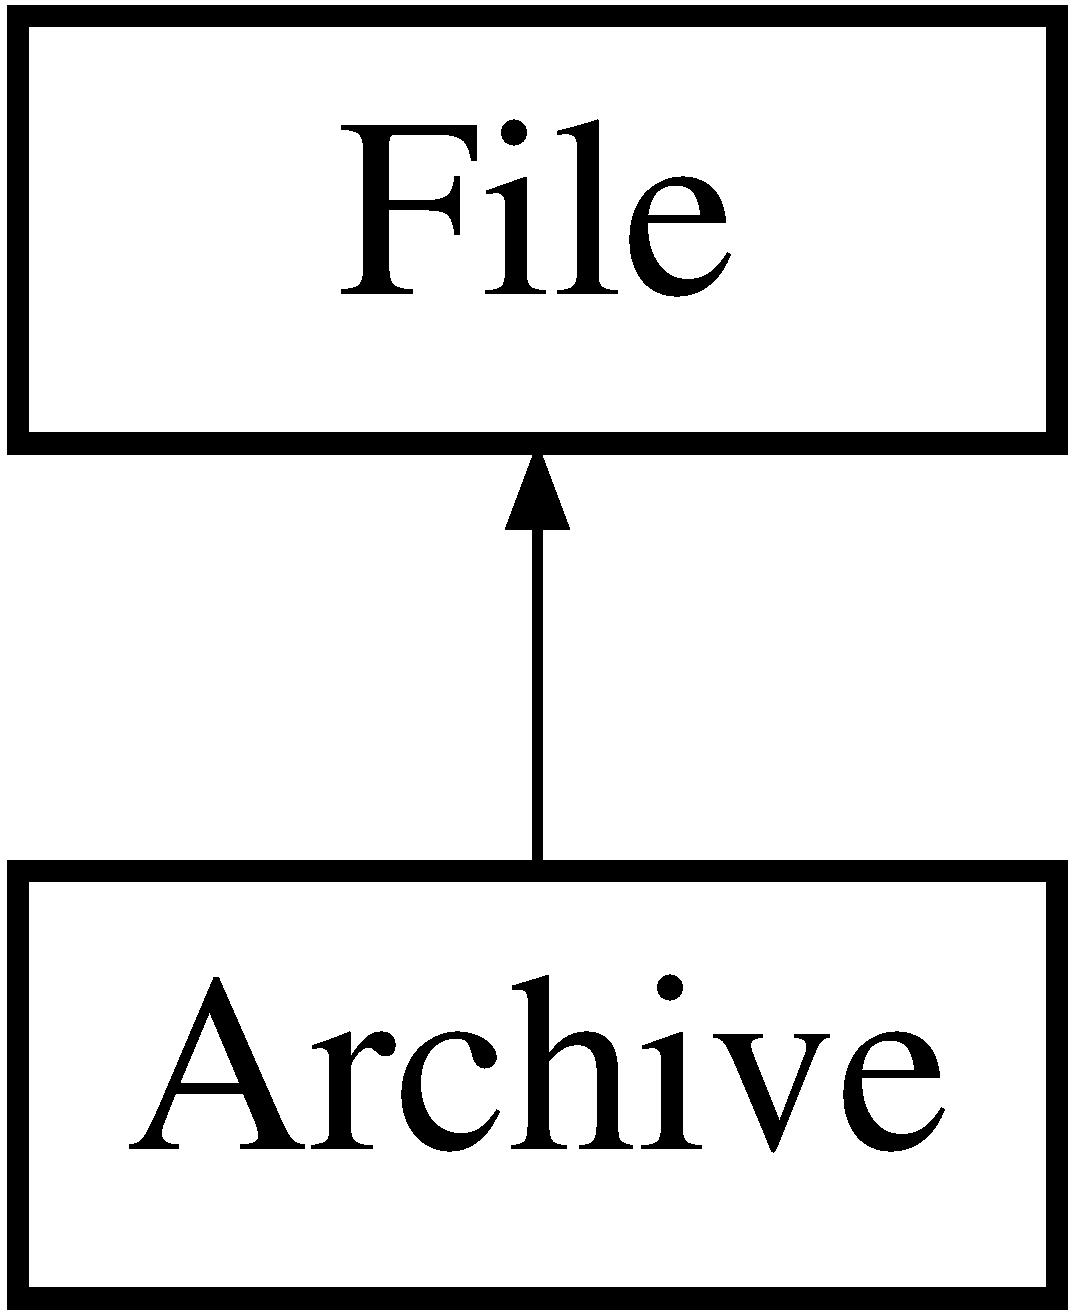
\includegraphics[height=2.000000cm]{class_archive}
\end{center}
\end{figure}
\subsection*{Public Member Functions}
\begin{DoxyCompactItemize}
\item 
\hyperlink{class_archive_aba703027bcdb0596c0dc46246b5efe4f}{Archive} (\hyperlink{class_r_a_r_options}{R\-A\-R\-Options} $\ast$Init\-Cmd=N\-U\-L\-L)
\item 
bool \hyperlink{class_archive_a5445c9c5db9e139d956946acf04d9aef}{Is\-Archive} (bool Enable\-Broken)
\item 
\hypertarget{class_archive_a11853cfd858d0fc9d5583723bfa62a54}{size\-\_\-t {\bfseries Search\-Block} (int Block\-Type)}\label{class_archive_a11853cfd858d0fc9d5583723bfa62a54}

\item 
\hypertarget{class_archive_a05db17b3fd4ef286bbba22e082855762}{size\-\_\-t {\bfseries Search\-Sub\-Block} (const char $\ast$Type)}\label{class_archive_a05db17b3fd4ef286bbba22e082855762}

\item 
\hypertarget{class_archive_a18c7f105189398c7d54f51befbb5427d}{int {\bfseries Read\-Block} (int Block\-Type)}\label{class_archive_a18c7f105189398c7d54f51befbb5427d}

\item 
\hypertarget{class_archive_a6cda3c976a6a5cc6608207cdde3628e8}{void {\bfseries Write\-Block} (int Block\-Type, \hyperlink{struct_base_block}{Base\-Block} $\ast$wb=N\-U\-L\-L)}\label{class_archive_a6cda3c976a6a5cc6608207cdde3628e8}

\item 
\hypertarget{class_archive_aa953c24ed872d504a5cc3c5ce8d5c39f}{int {\bfseries Prepare\-Names\-To\-Write} (char $\ast$Name, wchar $\ast$Name\-W, char $\ast$Dest\-Name, byte $\ast$Dest\-Name\-W)}\label{class_archive_aa953c24ed872d504a5cc3c5ce8d5c39f}

\item 
\hypertarget{class_archive_a1f401ed0535fdb5b7c84b3cf5a23b9cf}{void {\bfseries Set\-Lhd\-Size} ()}\label{class_archive_a1f401ed0535fdb5b7c84b3cf5a23b9cf}

\item 
\hypertarget{class_archive_a09aba5cbd51c0ac9aaaac5da5ac4ec22}{size\-\_\-t {\bfseries Read\-Header} ()}\label{class_archive_a09aba5cbd51c0ac9aaaac5da5ac4ec22}

\item 
\hypertarget{class_archive_aefe3b900bd528f5340070107e5aaf187}{void {\bfseries Check\-Arc} (bool Enable\-Broken)}\label{class_archive_aefe3b900bd528f5340070107e5aaf187}

\item 
\hypertarget{class_archive_a70ba18001ceb4090b91844fecff46b10}{void {\bfseries Check\-Open} (const char $\ast$Name, const wchar $\ast$Name\-W=N\-U\-L\-L)}\label{class_archive_a70ba18001ceb4090b91844fecff46b10}

\item 
\hypertarget{class_archive_ad9aedb27eb3fcd5848fc0be9d238eb1e}{bool {\bfseries W\-Check\-Open} (const char $\ast$Name, const wchar $\ast$Name\-W=N\-U\-L\-L)}\label{class_archive_ad9aedb27eb3fcd5848fc0be9d238eb1e}

\item 
\hypertarget{class_archive_a6f5a06a23d7b3fe0f2929f18f58056d8}{bool {\bfseries Get\-Comment} (\hyperlink{class_array}{Array}$<$ byte $>$ $\ast$Cmt\-Data, \hyperlink{class_array}{Array}$<$ wchar $>$ $\ast$Cmt\-Data\-W)}\label{class_archive_a6f5a06a23d7b3fe0f2929f18f58056d8}

\item 
\hypertarget{class_archive_a8e9c5a413ed09137211efaadbec15497}{void {\bfseries View\-Comment} ()}\label{class_archive_a8e9c5a413ed09137211efaadbec15497}

\item 
\hypertarget{class_archive_a0ee8d38d7e10c3082ff8920424d9ce71}{void {\bfseries View\-File\-Comment} ()}\label{class_archive_a0ee8d38d7e10c3082ff8920424d9ce71}

\item 
\hypertarget{class_archive_afb2478c77b30b6db8aa6f535dd34bb97}{void {\bfseries Set\-Latest\-Time} (\hyperlink{class_rar_time}{Rar\-Time} $\ast$New\-Time)}\label{class_archive_afb2478c77b30b6db8aa6f535dd34bb97}

\item 
\hypertarget{class_archive_a829861373cc7dee2c5cf8541e8474a8a}{void {\bfseries Seek\-To\-Next} ()}\label{class_archive_a829861373cc7dee2c5cf8541e8474a8a}

\item 
\hypertarget{class_archive_aee9f2dc996825c7bcf87f35e664ee597}{bool {\bfseries Check\-Access} ()}\label{class_archive_aee9f2dc996825c7bcf87f35e664ee597}

\item 
\hypertarget{class_archive_aab5d0e2308454b14301718daf08d3286}{bool {\bfseries Is\-Arc\-Dir} ()}\label{class_archive_aab5d0e2308454b14301718daf08d3286}

\item 
\hypertarget{class_archive_a1d7c46b19c25dea0c1fcae0fa8324049}{bool {\bfseries Is\-Arc\-Label} ()}\label{class_archive_a1d7c46b19c25dea0c1fcae0fa8324049}

\item 
\hypertarget{class_archive_ab068d6a33ef1cb87ace818fd454ed8da}{void {\bfseries Convert\-Attributes} ()}\label{class_archive_ab068d6a33ef1cb87ace818fd454ed8da}

\item 
\hypertarget{class_archive_ad5b9b5fbcfeb654595d6c3cb51d69144}{int {\bfseries Get\-Recovery\-Size} (bool Required)}\label{class_archive_ad5b9b5fbcfeb654595d6c3cb51d69144}

\item 
\hypertarget{class_archive_ac495c85ddc4f0b91c1bde4a8a2a019c4}{void {\bfseries Vol\-Subtract\-Header\-Size} (size\-\_\-t Sub\-Size)}\label{class_archive_ac495c85ddc4f0b91c1bde4a8a2a019c4}

\item 
\hypertarget{class_archive_a57d2e1f83e999a872db15691a7b0ec5c}{void {\bfseries Add\-Sub\-Data} (byte $\ast$Src\-Data, size\-\_\-t Data\-Size, \hyperlink{class_file}{File} $\ast$Src\-File, const char $\ast$Name, bool Allow\-Split)}\label{class_archive_a57d2e1f83e999a872db15691a7b0ec5c}

\item 
\hypertarget{class_archive_a005b58f3ac7bcfcc875cc9416f2f97da}{bool {\bfseries Read\-Sub\-Data} (\hyperlink{class_array}{Array}$<$ byte $>$ $\ast$Unp\-Data, \hyperlink{class_file}{File} $\ast$Dest\-File)}\label{class_archive_a005b58f3ac7bcfcc875cc9416f2f97da}

\item 
\hypertarget{class_archive_a190ef572a45ee772402e28f359b4f60b}{int {\bfseries Get\-Header\-Type} ()}\label{class_archive_a190ef572a45ee772402e28f359b4f60b}

\item 
\hypertarget{class_archive_a766b2eed7cae05eec0d82c824bcadedc}{size\-\_\-t {\bfseries Read\-Comment\-Data} (\hyperlink{class_array}{Array}$<$ byte $>$ $\ast$Cmt\-Data, \hyperlink{class_array}{Array}$<$ wchar $>$ $\ast$Cmt\-Data\-W)}\label{class_archive_a766b2eed7cae05eec0d82c824bcadedc}

\item 
\hypertarget{class_archive_a96ad955b4bcbaccc091f8c994950e583}{void {\bfseries Write\-Comment\-Data} (byte $\ast$Data, size\-\_\-t Data\-Size, bool File\-Comment)}\label{class_archive_a96ad955b4bcbaccc091f8c994950e583}

\item 
\hypertarget{class_archive_ab8bb60ec32cb017daa87b413947feb36}{\hyperlink{class_r_a_r_options}{R\-A\-R\-Options} $\ast$ {\bfseries Get\-R\-A\-R\-Options} ()}\label{class_archive_ab8bb60ec32cb017daa87b413947feb36}

\item 
\hypertarget{class_archive_a7dfd26057e52cc9ee075b6ed710a1b83}{void {\bfseries Set\-Silent\-Open} (bool Mode)}\label{class_archive_a7dfd26057e52cc9ee075b6ed710a1b83}

\item 
void \hyperlink{class_archive_a03292e03b219b4ba6f471891278252ed}{Init\-Arc} (byte $\ast$ptrlocation, int64 length)
\end{DoxyCompactItemize}
\subsection*{Public Attributes}
\begin{DoxyCompactItemize}
\item 
\hypertarget{class_archive_acc05c854ad71826bb9ff6272883e8f26}{\hyperlink{struct_base_block}{Base\-Block} {\bfseries Short\-Block}}\label{class_archive_acc05c854ad71826bb9ff6272883e8f26}

\item 
\hypertarget{class_archive_ac025c2c39107a9bd6f97dc40f8ebff5f}{\hyperlink{struct_main_header}{Main\-Header} {\bfseries New\-Mhd}}\label{class_archive_ac025c2c39107a9bd6f97dc40f8ebff5f}

\item 
\hypertarget{class_archive_a5e5f5d9249f75a89c7704ad75a5077db}{\hyperlink{struct_file_header}{File\-Header} {\bfseries New\-Lhd}}\label{class_archive_a5e5f5d9249f75a89c7704ad75a5077db}

\item 
\hypertarget{class_archive_a69016563cba9bae7bd8ae9b4fef5f46b}{\hyperlink{struct_end_arc_header}{End\-Arc\-Header} {\bfseries End\-Arc\-Head}}\label{class_archive_a69016563cba9bae7bd8ae9b4fef5f46b}

\item 
\hypertarget{class_archive_ad91a103801b3251b35d4872390fb1f97}{\hyperlink{struct_sub_block_header}{Sub\-Block\-Header} {\bfseries Sub\-Block\-Head}}\label{class_archive_ad91a103801b3251b35d4872390fb1f97}

\item 
\hypertarget{class_archive_abc557c567b59f2dd6a5931f6f4737811}{\hyperlink{struct_file_header}{File\-Header} {\bfseries Sub\-Head}}\label{class_archive_abc557c567b59f2dd6a5931f6f4737811}

\item 
\hypertarget{class_archive_aec0de971594058e613253397657acd7b}{\hyperlink{struct_comment_header}{Comment\-Header} {\bfseries Comm\-Head}}\label{class_archive_aec0de971594058e613253397657acd7b}

\item 
\hypertarget{class_archive_a02ab2a1e50eb7d17f1aa9805f24ccaad}{\hyperlink{struct_protect_header}{Protect\-Header} {\bfseries Protect\-Head}}\label{class_archive_a02ab2a1e50eb7d17f1aa9805f24ccaad}

\item 
\hypertarget{class_archive_a02a2939a52751daf0dcd2a024bcbafce}{\hyperlink{struct_a_v_header}{A\-V\-Header} {\bfseries A\-V\-Head}}\label{class_archive_a02a2939a52751daf0dcd2a024bcbafce}

\item 
\hypertarget{class_archive_af5f3d97448ed6d1a4f30561764f2a2a9}{\hyperlink{struct_sign_header}{Sign\-Header} {\bfseries Sign\-Head}}\label{class_archive_af5f3d97448ed6d1a4f30561764f2a2a9}

\item 
\hypertarget{class_archive_afeac4185b82bca80b550d89a1c2f3672}{\hyperlink{struct_unix_owners_header}{Unix\-Owners\-Header} {\bfseries U\-O\-Head}}\label{class_archive_afeac4185b82bca80b550d89a1c2f3672}

\item 
\hypertarget{class_archive_ac4da21a229265c65a9e4a1a39b2a1f2c}{\hyperlink{struct_mac_f_info_header}{Mac\-F\-Info\-Header} {\bfseries M\-A\-C\-Head}}\label{class_archive_ac4da21a229265c65a9e4a1a39b2a1f2c}

\item 
\hypertarget{class_archive_a1dbf61aeed5f00343fcab1e6f27fa6a6}{\hyperlink{struct_e_a_header}{E\-A\-Header} {\bfseries E\-A\-Head}}\label{class_archive_a1dbf61aeed5f00343fcab1e6f27fa6a6}

\item 
\hypertarget{class_archive_adba5ec5f6cbe0096f239ebaf114f934b}{\hyperlink{struct_stream_header}{Stream\-Header} {\bfseries Stream\-Head}}\label{class_archive_adba5ec5f6cbe0096f239ebaf114f934b}

\item 
\hypertarget{class_archive_aeaacc0f97d7b7cf63bf72961d6037c67}{int64 {\bfseries Cur\-Block\-Pos}}\label{class_archive_aeaacc0f97d7b7cf63bf72961d6037c67}

\item 
\hypertarget{class_archive_aad262f421de370a447886ff4a4074148}{int64 {\bfseries Next\-Block\-Pos}}\label{class_archive_aad262f421de370a447886ff4a4074148}

\item 
\hypertarget{class_archive_a08e4489c9c5b19a88316aeff6632b731}{bool {\bfseries Old\-Format}}\label{class_archive_a08e4489c9c5b19a88316aeff6632b731}

\item 
\hypertarget{class_archive_a856d6eeb17e700231ce9b18f3795f1b3}{bool {\bfseries Solid}}\label{class_archive_a856d6eeb17e700231ce9b18f3795f1b3}

\item 
\hypertarget{class_archive_afa19cf13ad715e4678f7be998a14a944}{bool {\bfseries Volume}}\label{class_archive_afa19cf13ad715e4678f7be998a14a944}

\item 
\hypertarget{class_archive_a90b9b1c93c01b2b64babafc0fb2a594d}{bool {\bfseries Main\-Comment}}\label{class_archive_a90b9b1c93c01b2b64babafc0fb2a594d}

\item 
\hypertarget{class_archive_a749caeec1dc9b303702facdc48e85082}{bool {\bfseries Locked}}\label{class_archive_a749caeec1dc9b303702facdc48e85082}

\item 
\hypertarget{class_archive_a14dd04fb01ebe41775eb65c639688c13}{bool {\bfseries Signed}}\label{class_archive_a14dd04fb01ebe41775eb65c639688c13}

\item 
\hypertarget{class_archive_a45d0d73f53cc7585e1c9b3d3e9cc5a09}{bool {\bfseries Not\-First\-Volume}}\label{class_archive_a45d0d73f53cc7585e1c9b3d3e9cc5a09}

\item 
\hypertarget{class_archive_a40ec5e95e99bda33df554558607a2f76}{bool {\bfseries Protected}}\label{class_archive_a40ec5e95e99bda33df554558607a2f76}

\item 
\hypertarget{class_archive_a1aae769bec37f8e04b17f2b9371e10c8}{bool {\bfseries Encrypted}}\label{class_archive_a1aae769bec37f8e04b17f2b9371e10c8}

\item 
\hypertarget{class_archive_ab3f26944af9bf02a1b058f77a2aa9fb8}{size\-\_\-t {\bfseries S\-F\-X\-Size}}\label{class_archive_ab3f26944af9bf02a1b058f77a2aa9fb8}

\item 
\hypertarget{class_archive_aae4c694138a3944d8f8bae637f9f19e9}{bool {\bfseries Broken\-File\-Header}}\label{class_archive_aae4c694138a3944d8f8bae637f9f19e9}

\item 
\hypertarget{class_archive_ac27ba87d6435ef47e7f607016e58171a}{bool {\bfseries Splitting}}\label{class_archive_ac27ba87d6435ef47e7f607016e58171a}

\item 
\hypertarget{class_archive_ad1cc015ff05618e66017354489f8fe0b}{ushort {\bfseries Header\-C\-R\-C}}\label{class_archive_ad1cc015ff05618e66017354489f8fe0b}

\item 
\hypertarget{class_archive_a57672b357cb2361e5c0ab9c434e74b79}{int64 {\bfseries Vol\-Write}}\label{class_archive_a57672b357cb2361e5c0ab9c434e74b79}

\item 
\hypertarget{class_archive_a7a83fe0946d71fec7dca7040e2efd7bf}{int64 {\bfseries Adding\-Files\-Size}}\label{class_archive_a7a83fe0946d71fec7dca7040e2efd7bf}

\item 
\hypertarget{class_archive_aeeae6c53f82644fb1379843b817bd7b7}{size\-\_\-t {\bfseries Adding\-Headers\-Size}}\label{class_archive_aeeae6c53f82644fb1379843b817bd7b7}

\item 
\hypertarget{class_archive_af7c3883f298817985fe1e4e74c1eda71}{bool {\bfseries New\-Archive}}\label{class_archive_af7c3883f298817985fe1e4e74c1eda71}

\item 
\hypertarget{class_archive_af516db7923f3ceff3da8e51cadf46a5c}{char {\bfseries First\-Volume\-Name} \mbox{[}N\-M\mbox{]}}\label{class_archive_af516db7923f3ceff3da8e51cadf46a5c}

\item 
\hypertarget{class_archive_a9be06505fbb4f9aee2ec8fd19f85b115}{wchar {\bfseries First\-Volume\-Name\-W} \mbox{[}N\-M\mbox{]}}\label{class_archive_a9be06505fbb4f9aee2ec8fd19f85b115}

\end{DoxyCompactItemize}
\subsection*{Additional Inherited Members}


\subsection{Detailed Description}
This class handles the reading of a Roshal A\-Rchive. It is able to unpack, decompress, and decrypt data. 

\subsection{Constructor \& Destructor Documentation}
\hypertarget{class_archive_aba703027bcdb0596c0dc46246b5efe4f}{\index{Archive@{Archive}!Archive@{Archive}}
\index{Archive@{Archive}!Archive@{Archive}}
\subsubsection[{Archive}]{\setlength{\rightskip}{0pt plus 5cm}Archive\-::\-Archive (
\begin{DoxyParamCaption}
\item[{{\bf R\-A\-R\-Options} $\ast$}]{Init\-Cmd = {\ttfamily NULL}}
\end{DoxyParamCaption}
)}}\label{class_archive_aba703027bcdb0596c0dc46246b5efe4f}
Special Constructor 

\subsection{Member Function Documentation}
\hypertarget{class_archive_a03292e03b219b4ba6f471891278252ed}{\index{Archive@{Archive}!Init\-Arc@{Init\-Arc}}
\index{Init\-Arc@{Init\-Arc}!Archive@{Archive}}
\subsubsection[{Init\-Arc}]{\setlength{\rightskip}{0pt plus 5cm}void Archive\-::\-Init\-Arc (
\begin{DoxyParamCaption}
\item[{byte $\ast$}]{ptrlocation, }
\item[{int64}]{length}
\end{DoxyParamCaption}
)}}\label{class_archive_a03292e03b219b4ba6f471891278252ed}
This function must be called after an archive has been instantiated. This sets up the archive to read from the {\ttfamily \hyperlink{class_file}{File}} class. 
\begin{DoxyParams}{Parameters}
{\em ptrlocation} & -\/ a location in memory where the R\-A\-R file begins \\
\hline
{\em length} & -\/ the length of the memory location that can be read \\
\hline
\end{DoxyParams}
\hypertarget{class_archive_a5445c9c5db9e139d956946acf04d9aef}{\index{Archive@{Archive}!Is\-Archive@{Is\-Archive}}
\index{Is\-Archive@{Is\-Archive}!Archive@{Archive}}
\subsubsection[{Is\-Archive}]{\setlength{\rightskip}{0pt plus 5cm}bool Archive\-::\-Is\-Archive (
\begin{DoxyParamCaption}
\item[{bool}]{Enable\-Broken}
\end{DoxyParamCaption}
)}}\label{class_archive_a5445c9c5db9e139d956946acf04d9aef}
Checks to make sure that an archive actually exists 
\begin{DoxyParams}{Parameters}
{\em Enable\-Broken} & -\/ makes the archive opening process continue even when errors occur \\
\hline
\end{DoxyParams}


The documentation for this class was generated from the following files\-:\begin{DoxyCompactItemize}
\item 
/\-Users/salazbr1/\-Documents/\-N\-P\-S/final\-\_\-unrarbulk\-\_\-extractor\-\_\-07-\/26-\/12/code/archive.\-hpp\item 
/\-Users/salazbr1/\-Documents/\-N\-P\-S/final\-\_\-unrarbulk\-\_\-extractor\-\_\-07-\/26-\/12/code/arccmt.\-cpp\item 
/\-Users/salazbr1/\-Documents/\-N\-P\-S/final\-\_\-unrarbulk\-\_\-extractor\-\_\-07-\/26-\/12/code/archive.\-cpp\item 
/\-Users/salazbr1/\-Documents/\-N\-P\-S/final\-\_\-unrarbulk\-\_\-extractor\-\_\-07-\/26-\/12/code/arcread.\-cpp\end{DoxyCompactItemize}

\hypertarget{class_array}{\section{Array$<$ T $>$ Class Template Reference}
\label{class_array}\index{Array$<$ T $>$@{Array$<$ T $>$}}
}
\subsection*{Public Member Functions}
\begin{DoxyCompactItemize}
\item 
\hypertarget{class_array_a76b75c2b76210689c42d6a3966b2bbb4}{{\bfseries Array} (size\-\_\-t Size)}\label{class_array_a76b75c2b76210689c42d6a3966b2bbb4}

\item 
\hypertarget{class_array_a9c4bde1217ea8505dd7cbf4543402e91}{void {\bfseries Clean\-Data} ()}\label{class_array_a9c4bde1217ea8505dd7cbf4543402e91}

\item 
\hypertarget{class_array_ad89a95323691b7a5f34b2ef10d59cd2c}{T \& {\bfseries operator\mbox{[}$\,$\mbox{]}} (size\-\_\-t Item)}\label{class_array_ad89a95323691b7a5f34b2ef10d59cd2c}

\item 
\hypertarget{class_array_a769e23dfe90cfd7ad1f55d771d164644}{size\-\_\-t {\bfseries Size} ()}\label{class_array_a769e23dfe90cfd7ad1f55d771d164644}

\item 
\hypertarget{class_array_a8173b0dc2fb6d869bdd8ee0da49cb8a7}{void {\bfseries Add} (size\-\_\-t Items)}\label{class_array_a8173b0dc2fb6d869bdd8ee0da49cb8a7}

\item 
\hypertarget{class_array_aa321acfbc75a9f248c0607d690890087}{void {\bfseries Alloc} (size\-\_\-t Items)}\label{class_array_aa321acfbc75a9f248c0607d690890087}

\item 
\hypertarget{class_array_a9676592932b3b1b43fdd2fd80baed764}{void {\bfseries Reset} ()}\label{class_array_a9676592932b3b1b43fdd2fd80baed764}

\item 
\hypertarget{class_array_a76e715e60794c3b71e385e05f4761a8b}{void {\bfseries operator=} (\hyperlink{class_array}{Array}$<$ T $>$ \&Src)}\label{class_array_a76e715e60794c3b71e385e05f4761a8b}

\item 
\hypertarget{class_array_ad3773cbc7c7b8a865f448fc8f74658aa}{void {\bfseries Push} (T Item)}\label{class_array_ad3773cbc7c7b8a865f448fc8f74658aa}

\item 
\hypertarget{class_array_ad9faf2ae8a9aa0a63fed50d273e97a56}{T $\ast$ {\bfseries Addr} ()}\label{class_array_ad9faf2ae8a9aa0a63fed50d273e97a56}

\end{DoxyCompactItemize}


The documentation for this class was generated from the following file\-:\begin{DoxyCompactItemize}
\item 
/\-Users/salazbr1/\-Documents/\-N\-P\-S/final\-\_\-unrarbulk\-\_\-extractor\-\_\-07-\/26-\/12/code/array.\-hpp\end{DoxyCompactItemize}

\hypertarget{struct_audio_variables}{\section{Audio\-Variables Struct Reference}
\label{struct_audio_variables}\index{Audio\-Variables@{Audio\-Variables}}
}
\subsection*{Public Attributes}
\begin{DoxyCompactItemize}
\item 
\hypertarget{struct_audio_variables_ad31c92d12433269f2e624e891fa16860}{int {\bfseries K1}}\label{struct_audio_variables_ad31c92d12433269f2e624e891fa16860}

\item 
\hypertarget{struct_audio_variables_a2a88b0c4ccb8ae660acf8b40007b3b6f}{int {\bfseries K2}}\label{struct_audio_variables_a2a88b0c4ccb8ae660acf8b40007b3b6f}

\item 
\hypertarget{struct_audio_variables_ad10b9136e6c185d9df8184a3266b2f9e}{int {\bfseries K3}}\label{struct_audio_variables_ad10b9136e6c185d9df8184a3266b2f9e}

\item 
\hypertarget{struct_audio_variables_a8c585051f60d4ad7ad3ab3f29a83f4ad}{int {\bfseries K4}}\label{struct_audio_variables_a8c585051f60d4ad7ad3ab3f29a83f4ad}

\item 
\hypertarget{struct_audio_variables_a68fc9b3c3ad5386a141341ae8c408796}{int {\bfseries K5}}\label{struct_audio_variables_a68fc9b3c3ad5386a141341ae8c408796}

\item 
\hypertarget{struct_audio_variables_a7e69ac2e1572bc4cc99e9db7da30e940}{int {\bfseries D1}}\label{struct_audio_variables_a7e69ac2e1572bc4cc99e9db7da30e940}

\item 
\hypertarget{struct_audio_variables_aa8421d20ce1d969e9c350953f16ef037}{int {\bfseries D2}}\label{struct_audio_variables_aa8421d20ce1d969e9c350953f16ef037}

\item 
\hypertarget{struct_audio_variables_a5c1918b645b70bbb21257d73d918e098}{int {\bfseries D3}}\label{struct_audio_variables_a5c1918b645b70bbb21257d73d918e098}

\item 
\hypertarget{struct_audio_variables_a0bb6d88248bf70c611364ad575a3ee28}{int {\bfseries D4}}\label{struct_audio_variables_a0bb6d88248bf70c611364ad575a3ee28}

\item 
\hypertarget{struct_audio_variables_adb319d2275d33de3f8116a5c078288b1}{int {\bfseries Last\-Delta}}\label{struct_audio_variables_adb319d2275d33de3f8116a5c078288b1}

\item 
\hypertarget{struct_audio_variables_aaca37e0796ab40ea58cfd6017368633b}{unsigned int {\bfseries Dif} \mbox{[}11\mbox{]}}\label{struct_audio_variables_aaca37e0796ab40ea58cfd6017368633b}

\item 
\hypertarget{struct_audio_variables_adf2f28e8a4c3c9ed195182364c85438f}{unsigned int {\bfseries Byte\-Count}}\label{struct_audio_variables_adf2f28e8a4c3c9ed195182364c85438f}

\item 
\hypertarget{struct_audio_variables_af33b9ced85af0976a5d66567488852c4}{int {\bfseries Last\-Char}}\label{struct_audio_variables_af33b9ced85af0976a5d66567488852c4}

\end{DoxyCompactItemize}


The documentation for this struct was generated from the following file\-:\begin{DoxyCompactItemize}
\item 
/\-Users/salazbr1/\-Documents/\-N\-P\-S/final\-\_\-unrarbulk\-\_\-extractor\-\_\-07-\/26-\/12/code/unpack.\-hpp\end{DoxyCompactItemize}

\hypertarget{struct_a_v_header}{\section{A\-V\-Header Struct Reference}
\label{struct_a_v_header}\index{A\-V\-Header@{A\-V\-Header}}
}
Inheritance diagram for A\-V\-Header\-:\begin{figure}[H]
\begin{center}
\leavevmode
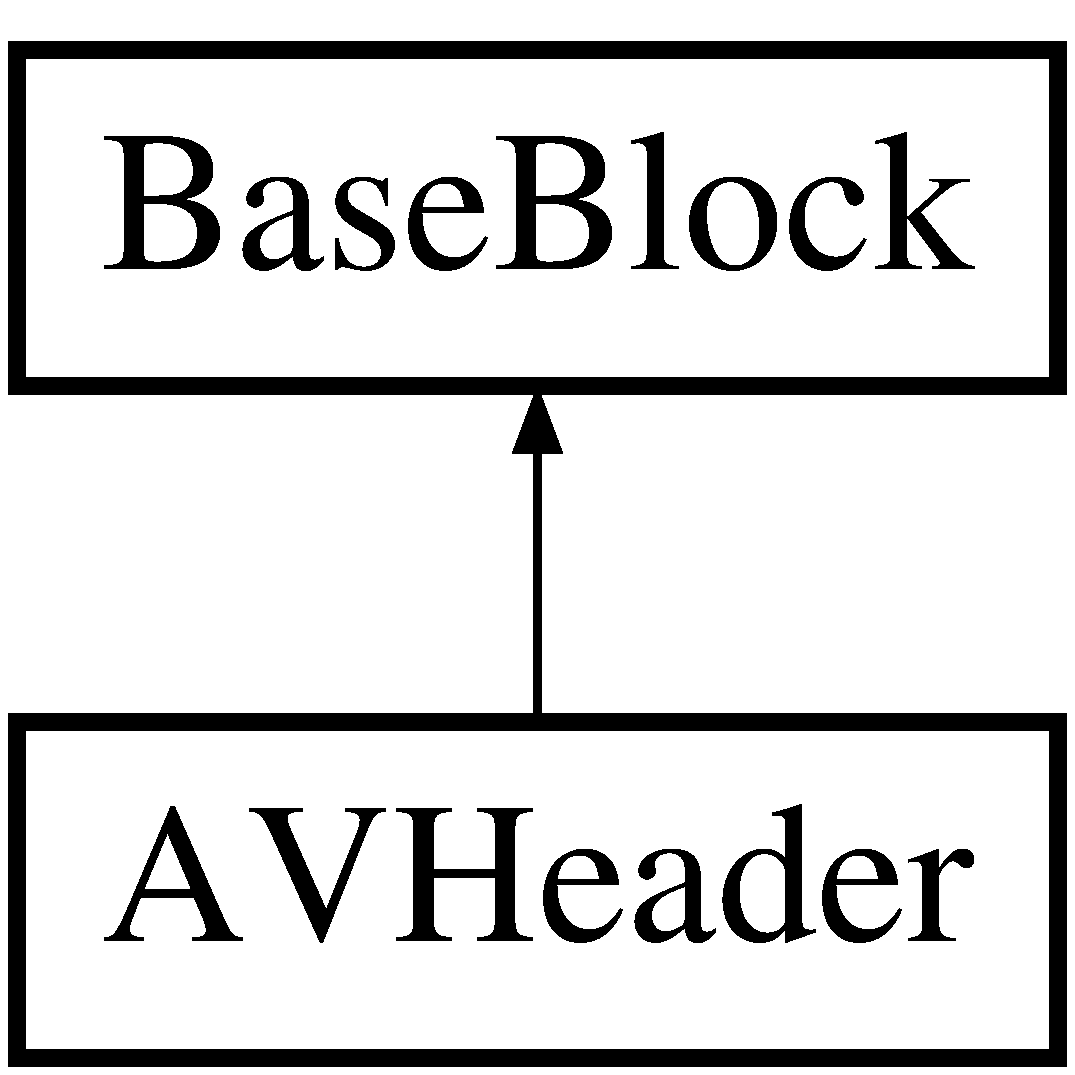
\includegraphics[height=2.000000cm]{struct_a_v_header}
\end{center}
\end{figure}
\subsection*{Public Attributes}
\begin{DoxyCompactItemize}
\item 
\hypertarget{struct_a_v_header_aa8b96dc3302838d9f5ece7bdb5a474b0}{byte {\bfseries Unp\-Ver}}\label{struct_a_v_header_aa8b96dc3302838d9f5ece7bdb5a474b0}

\item 
\hypertarget{struct_a_v_header_a3f28e3850c904233913f909622939dfc}{byte {\bfseries Method}}\label{struct_a_v_header_a3f28e3850c904233913f909622939dfc}

\item 
\hypertarget{struct_a_v_header_a6d3f15088c1aec8742727529edb27041}{byte {\bfseries A\-V\-Ver}}\label{struct_a_v_header_a6d3f15088c1aec8742727529edb27041}

\item 
\hypertarget{struct_a_v_header_a0e4d520a6f97df32b41b5b6c364aa498}{uint {\bfseries A\-V\-Info\-C\-R\-C}}\label{struct_a_v_header_a0e4d520a6f97df32b41b5b6c364aa498}

\end{DoxyCompactItemize}
\subsection*{Additional Inherited Members}


The documentation for this struct was generated from the following file\-:\begin{DoxyCompactItemize}
\item 
/\-Users/salazbr1/\-Documents/\-N\-P\-S/final\-\_\-unrarbulk\-\_\-extractor\-\_\-07-\/26-\/12/code/headers.\-hpp\end{DoxyCompactItemize}

\hypertarget{struct_base_block}{\section{Base\-Block Struct Reference}
\label{struct_base_block}\index{Base\-Block@{Base\-Block}}
}
Inheritance diagram for Base\-Block\-:\begin{figure}[H]
\begin{center}
\leavevmode
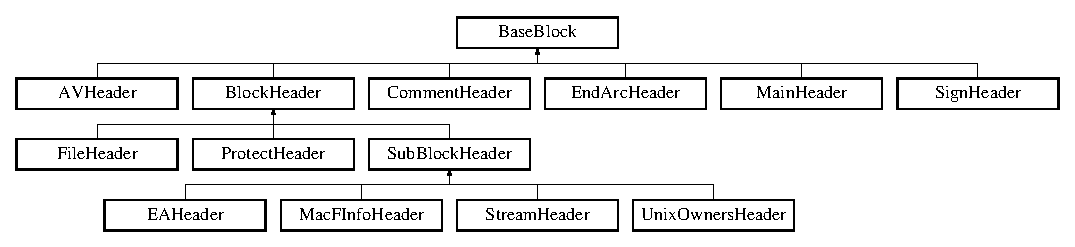
\includegraphics[height=2.871795cm]{struct_base_block}
\end{center}
\end{figure}
\subsection*{Public Member Functions}
\begin{DoxyCompactItemize}
\item 
\hypertarget{struct_base_block_a9eaebe3621abca92a6f9369dd7fb3c15}{bool {\bfseries Is\-Sub\-Block} ()}\label{struct_base_block_a9eaebe3621abca92a6f9369dd7fb3c15}

\end{DoxyCompactItemize}
\subsection*{Public Attributes}
\begin{DoxyCompactItemize}
\item 
\hypertarget{struct_base_block_a3f9faebc338b925dff7251eaa12b6125}{ushort {\bfseries Head\-C\-R\-C}}\label{struct_base_block_a3f9faebc338b925dff7251eaa12b6125}

\item 
\hypertarget{struct_base_block_a4ca02caaefa3e091567787dfe370cc00}{H\-E\-A\-D\-E\-R\-\_\-\-T\-Y\-P\-E {\bfseries Head\-Type}}\label{struct_base_block_a4ca02caaefa3e091567787dfe370cc00}

\item 
\hypertarget{struct_base_block_a99236589d620b6635717cf5800687253}{ushort {\bfseries Flags}}\label{struct_base_block_a99236589d620b6635717cf5800687253}

\item 
\hypertarget{struct_base_block_a2de5de50cce54eab3b72e8ff7bef15bd}{ushort {\bfseries Head\-Size}}\label{struct_base_block_a2de5de50cce54eab3b72e8ff7bef15bd}

\end{DoxyCompactItemize}


The documentation for this struct was generated from the following file\-:\begin{DoxyCompactItemize}
\item 
/\-Users/salazbr1/\-Documents/\-N\-P\-S/final\-\_\-unrarbulk\-\_\-extractor\-\_\-07-\/26-\/12/code/headers.\-hpp\end{DoxyCompactItemize}

\hypertarget{class_bit_input}{\section{Bit\-Input Class Reference}
\label{class_bit_input}\index{Bit\-Input@{Bit\-Input}}
}
Inheritance diagram for Bit\-Input\-:\begin{figure}[H]
\begin{center}
\leavevmode
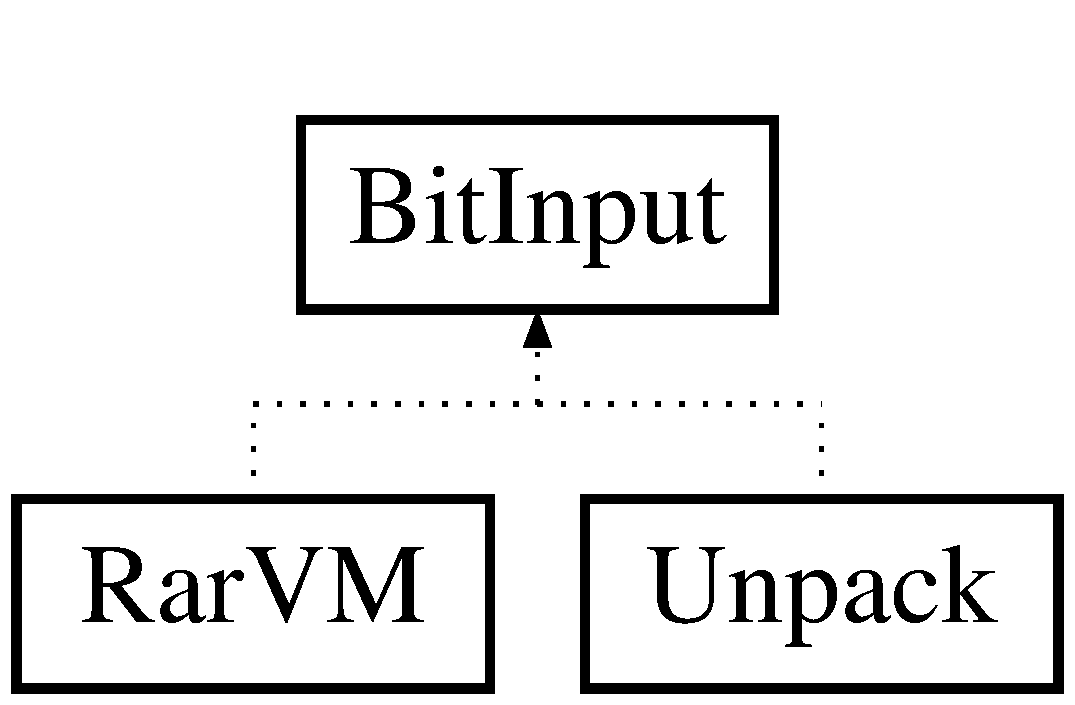
\includegraphics[height=2.000000cm]{class_bit_input}
\end{center}
\end{figure}
\subsection*{Public Types}
\begin{DoxyCompactItemize}
\item 
enum {\bfseries Buffer\-Size} \{ {\bfseries M\-A\-X\-\_\-\-S\-I\-Z\-E} = 0x8000
 \}
\end{DoxyCompactItemize}
\subsection*{Public Member Functions}
\begin{DoxyCompactItemize}
\item 
\hypertarget{class_bit_input_afa023e3612918c9b1c7b7af04e72c665}{void {\bfseries Init\-Bit\-Input} ()}\label{class_bit_input_afa023e3612918c9b1c7b7af04e72c665}

\item 
\hypertarget{class_bit_input_ab996a671a72ba39cd72fa654d17dd043}{void {\bfseries addbits} (uint Bits)}\label{class_bit_input_ab996a671a72ba39cd72fa654d17dd043}

\item 
\hypertarget{class_bit_input_a83f6fc69abea5ce4f84af537d0fa5307}{uint {\bfseries getbits} ()}\label{class_bit_input_a83f6fc69abea5ce4f84af537d0fa5307}

\item 
\hypertarget{class_bit_input_ad9d7dab7ad2ce436824c0241441304f9}{void {\bfseries faddbits} (uint Bits)}\label{class_bit_input_ad9d7dab7ad2ce436824c0241441304f9}

\item 
\hypertarget{class_bit_input_a74d822074d53902c6cc4c5803ac91131}{uint {\bfseries fgetbits} ()}\label{class_bit_input_a74d822074d53902c6cc4c5803ac91131}

\item 
\hypertarget{class_bit_input_a3d66ad2c5cf16bb4ac41f6ad2f6baf0e}{bool {\bfseries Overflow} (uint Inc\-Ptr)}\label{class_bit_input_a3d66ad2c5cf16bb4ac41f6ad2f6baf0e}

\end{DoxyCompactItemize}
\subsection*{Public Attributes}
\begin{DoxyCompactItemize}
\item 
\hypertarget{class_bit_input_af86e47d05a107bcd633e19870ff4b18c}{byte $\ast$ {\bfseries In\-Buf}}\label{class_bit_input_af86e47d05a107bcd633e19870ff4b18c}

\end{DoxyCompactItemize}
\subsection*{Protected Attributes}
\begin{DoxyCompactItemize}
\item 
\hypertarget{class_bit_input_ae497d2964eaf24014487514ee8b67bb1}{int {\bfseries In\-Addr}}\label{class_bit_input_ae497d2964eaf24014487514ee8b67bb1}

\item 
\hypertarget{class_bit_input_a5644c81728aa364fda230975bf73f371}{int {\bfseries In\-Bit}}\label{class_bit_input_a5644c81728aa364fda230975bf73f371}

\end{DoxyCompactItemize}


The documentation for this class was generated from the following files\-:\begin{DoxyCompactItemize}
\item 
/\-Users/salazbr1/\-Documents/\-N\-P\-S/final\-\_\-unrarbulk\-\_\-extractor\-\_\-07-\/26-\/12/code/getbits.\-hpp\item 
/\-Users/salazbr1/\-Documents/\-N\-P\-S/final\-\_\-unrarbulk\-\_\-extractor\-\_\-07-\/26-\/12/code/getbits.\-cpp\end{DoxyCompactItemize}

\hypertarget{struct_block_header}{\section{Block\-Header Struct Reference}
\label{struct_block_header}\index{Block\-Header@{Block\-Header}}
}
Inheritance diagram for Block\-Header\-:\begin{figure}[H]
\begin{center}
\leavevmode
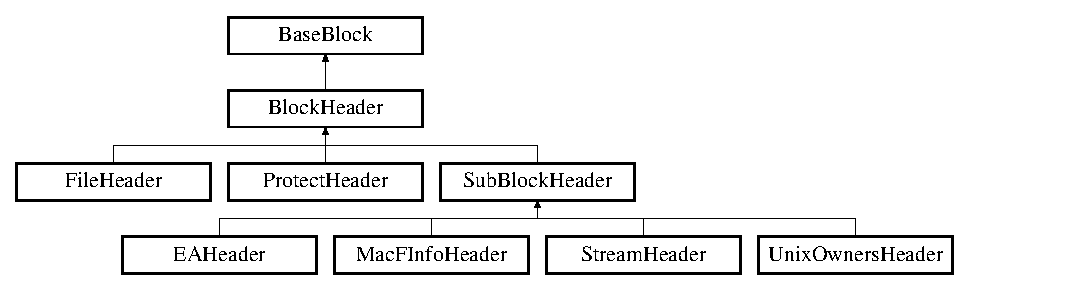
\includegraphics[height=3.446154cm]{struct_block_header}
\end{center}
\end{figure}
\subsection*{Public Attributes}
\begin{DoxyCompactItemize}
\item 
\hypertarget{struct_block_header_a6cbd4f4b4b19f1bc327ded68414a5023}{\begin{tabbing}
xx\=xx\=xx\=xx\=xx\=xx\=xx\=xx\=xx\=\kill
union \{\\
\>uint {\bfseries DataSize}\\
\>uint {\bfseries PackSize}\\
\}; }\label{struct_block_header_a6cbd4f4b4b19f1bc327ded68414a5023}
\\

\end{tabbing}\end{DoxyCompactItemize}
\subsection*{Additional Inherited Members}


The documentation for this struct was generated from the following file\-:\begin{DoxyCompactItemize}
\item 
/\-Users/salazbr1/\-Documents/\-N\-P\-S/final\-\_\-unrarbulk\-\_\-extractor\-\_\-07-\/26-\/12/code/headers.\-hpp\end{DoxyCompactItemize}

\hypertarget{class_cmd_extract}{\section{Cmd\-Extract Class Reference}
\label{class_cmd_extract}\index{Cmd\-Extract@{Cmd\-Extract}}
}
\subsection*{Public Member Functions}
\begin{DoxyCompactItemize}
\item 
\hypertarget{class_cmd_extract_a7d159412140281287271694ba881d596}{void {\bfseries Do\-Extract} (\hyperlink{class_command_data}{Command\-Data} $\ast$Cmd, byte $\ast$ptrlocation, int64 length, std\-::string \&xml)}\label{class_cmd_extract_a7d159412140281287271694ba881d596}

\item 
\hypertarget{class_cmd_extract_a85bd068da65d48061a194ddadeabd362}{void {\bfseries Extract\-Archive\-Init} (\hyperlink{class_command_data}{Command\-Data} $\ast$Cmd, \hyperlink{class_archive}{Archive} \&Arc)}\label{class_cmd_extract_a85bd068da65d48061a194ddadeabd362}

\item 
\hypertarget{class_cmd_extract_a1cd4ef7fdd2a73302dd65a5c4aa0b774}{bool {\bfseries Extract\-Current\-File} (\hyperlink{class_command_data}{Command\-Data} $\ast$Cmd, \hyperlink{class_archive}{Archive} \&Arc, size\-\_\-t Header\-Size, bool \&Repeat, std\-::string \&xml)}\label{class_cmd_extract_a1cd4ef7fdd2a73302dd65a5c4aa0b774}

\item 
\hypertarget{class_cmd_extract_a283db4b2aff0607b9a622f3b7343be9b}{void {\bfseries Set\-Compr\-Data\-I\-O} (\hyperlink{class_compr_data_i_o}{Compr\-Data\-I\-O} dataio)}\label{class_cmd_extract_a283db4b2aff0607b9a622f3b7343be9b}

\end{DoxyCompactItemize}
\subsection*{Static Public Member Functions}
\begin{DoxyCompactItemize}
\item 
\hypertarget{class_cmd_extract_a5433c944c5958cf99ff205e5903e3da6}{static void {\bfseries Unstore\-File} (\hyperlink{class_compr_data_i_o}{Compr\-Data\-I\-O} \&Data\-I\-O, int64 Dest\-Unp\-Size)}\label{class_cmd_extract_a5433c944c5958cf99ff205e5903e3da6}

\end{DoxyCompactItemize}
\subsection*{Public Attributes}
\begin{DoxyCompactItemize}
\item 
\hypertarget{class_cmd_extract_a1b2ad1984fde266e359bc910a80575cf}{bool {\bfseries Signature\-Found}}\label{class_cmd_extract_a1b2ad1984fde266e359bc910a80575cf}

\end{DoxyCompactItemize}


The documentation for this class was generated from the following files\-:\begin{DoxyCompactItemize}
\item 
/\-Users/salazbr1/\-Documents/\-N\-P\-S/final\-\_\-unrarbulk\-\_\-extractor\-\_\-07-\/26-\/12/code/extract.\-hpp\item 
/\-Users/salazbr1/\-Documents/\-N\-P\-S/final\-\_\-unrarbulk\-\_\-extractor\-\_\-07-\/26-\/12/code/extract.\-cpp\end{DoxyCompactItemize}

\hypertarget{class_command_data}{\section{Command\-Data Class Reference}
\label{class_command_data}\index{Command\-Data@{Command\-Data}}
}
Inheritance diagram for Command\-Data\-:\begin{figure}[H]
\begin{center}
\leavevmode
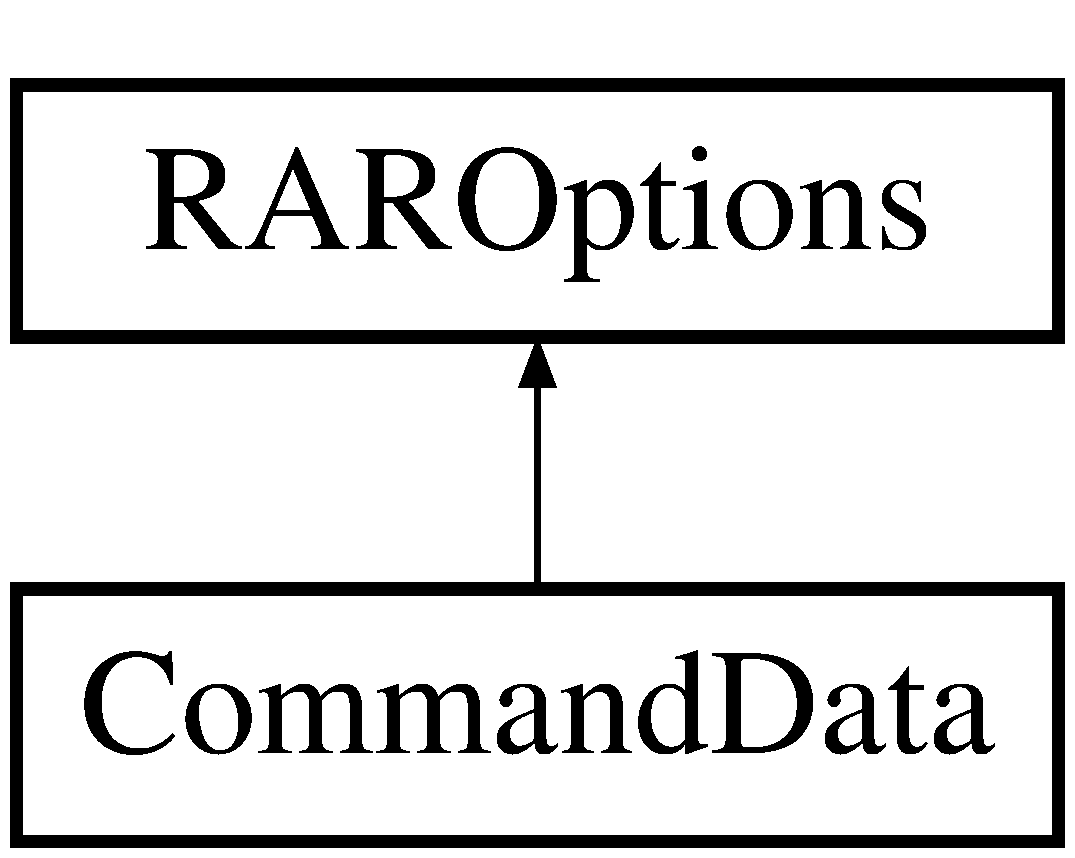
\includegraphics[height=2.000000cm]{class_command_data}
\end{center}
\end{figure}
\subsection*{Public Member Functions}
\begin{DoxyCompactItemize}
\item 
\hypertarget{class_command_data_ad63d5695cbc3d8aec1795cd4d258e47e}{void {\bfseries Init} ()}\label{class_command_data_ad63d5695cbc3d8aec1795cd4d258e47e}

\item 
\hypertarget{class_command_data_a3b7758bea130948a31e5fa70c07d0006}{void {\bfseries Close} ()}\label{class_command_data_a3b7758bea130948a31e5fa70c07d0006}

\item 
\hypertarget{class_command_data_a0547939cdb4f52fc7acf6cb260021d87}{void {\bfseries Preprocess\-Command\-Line} (int argc, char $\ast$argv\mbox{[}$\,$\mbox{]})}\label{class_command_data_a0547939cdb4f52fc7acf6cb260021d87}

\item 
\hypertarget{class_command_data_ab984187a6f60d79d5dd0277b890945b0}{void {\bfseries Parse\-Command\-Line} (int argc, char $\ast$argv\mbox{[}$\,$\mbox{]})}\label{class_command_data_ab984187a6f60d79d5dd0277b890945b0}

\item 
\hypertarget{class_command_data_adce9f02e44d1ef88a4414ffa850cb63e}{void {\bfseries Parse\-Arg} (char $\ast$Arg, wchar $\ast$Arg\-W)}\label{class_command_data_adce9f02e44d1ef88a4414ffa850cb63e}

\item 
\hypertarget{class_command_data_ad70249d7eac21f97d90156503fbd9ade}{void {\bfseries Parse\-Done} ()}\label{class_command_data_ad70249d7eac21f97d90156503fbd9ade}

\item 
\hypertarget{class_command_data_ac57a44878f6473a9a0a3cc2ee8e5a467}{void {\bfseries Parse\-Env\-Var} ()}\label{class_command_data_ac57a44878f6473a9a0a3cc2ee8e5a467}

\item 
\hypertarget{class_command_data_a037030ad1b69ae743ace05bc4c427ecc}{void {\bfseries Read\-Config} ()}\label{class_command_data_a037030ad1b69ae743ace05bc4c427ecc}

\item 
\hypertarget{class_command_data_ab4927ff8058e589a2906fbb78e271c98}{bool {\bfseries Preprocess\-Switch} (const char $\ast$Switch)}\label{class_command_data_ab4927ff8058e589a2906fbb78e271c98}

\item 
\hypertarget{class_command_data_a9e482d22652482c99ac7c8922d26af3f}{void {\bfseries Out\-Title} ()}\label{class_command_data_a9e482d22652482c99ac7c8922d26af3f}

\item 
\hypertarget{class_command_data_a34ea00f5ec9a583b8006c4a4b328bf8c}{void {\bfseries Out\-Help} ()}\label{class_command_data_a34ea00f5ec9a583b8006c4a4b328bf8c}

\item 
\hypertarget{class_command_data_ac544b0af528d04f4d7ffe890980531e2}{bool {\bfseries Is\-Switch} (int Ch)}\label{class_command_data_ac544b0af528d04f4d7ffe890980531e2}

\item 
\hypertarget{class_command_data_aaef8a202792a0f423dc4e64b02ef2e06}{bool {\bfseries Excl\-Check} (char $\ast$Check\-Name, bool Dir, bool Check\-Full\-Path, bool Check\-Incl\-List)}\label{class_command_data_aaef8a202792a0f423dc4e64b02ef2e06}

\item 
\hypertarget{class_command_data_afef640707c5192a4cbb1f7d7083160e2}{bool {\bfseries Excl\-Dir\-By\-Attr} (uint File\-Attr)}\label{class_command_data_afef640707c5192a4cbb1f7d7083160e2}

\item 
\hypertarget{class_command_data_a191bf7d1c9cf0b562f690d27beec2962}{bool {\bfseries Time\-Check} (\hyperlink{class_rar_time}{Rar\-Time} \&ft)}\label{class_command_data_a191bf7d1c9cf0b562f690d27beec2962}

\item 
\hypertarget{class_command_data_a8bf113973a5ce01845d8844a9d8da78a}{bool {\bfseries Size\-Check} (int64 Size)}\label{class_command_data_a8bf113973a5ce01845d8844a9d8da78a}

\item 
\hypertarget{class_command_data_a763c769904166ac782fec361fbe432ab}{bool {\bfseries Any\-Filters\-Active} ()}\label{class_command_data_a763c769904166ac782fec361fbe432ab}

\item 
\hypertarget{class_command_data_a0b202f0e462764cd26bcc5804e9eabdd}{int {\bfseries Is\-Process\-File} (\hyperlink{struct_file_header}{File\-Header} \&New\-Lhd, bool $\ast$Exact\-Match=N\-U\-L\-L, int Match\-Type=M\-A\-T\-C\-H\-\_\-\-W\-I\-L\-D\-S\-U\-B\-P\-A\-T\-H)}\label{class_command_data_a0b202f0e462764cd26bcc5804e9eabdd}

\item 
\hypertarget{class_command_data_ae5592e260e8c12f79780dbb22f8d8ff6}{void {\bfseries Process\-Command} ()}\label{class_command_data_ae5592e260e8c12f79780dbb22f8d8ff6}

\item 
\hypertarget{class_command_data_aa4ac3e304700100b5fa68fce8eec5c92}{void {\bfseries Add\-Arc\-Name} (const char $\ast$Name, const wchar $\ast$Name\-W)}\label{class_command_data_aa4ac3e304700100b5fa68fce8eec5c92}

\item 
\hypertarget{class_command_data_a138b2c28820fa4007a963f573b7867c3}{bool {\bfseries Get\-Arc\-Name} (char $\ast$Name, wchar $\ast$Name\-W, int Max\-Size)}\label{class_command_data_a138b2c28820fa4007a963f573b7867c3}

\item 
\hypertarget{class_command_data_a9dcc3420dd5e7147d1e3e227727da477}{bool {\bfseries Check\-Win\-Size} ()}\label{class_command_data_a9dcc3420dd5e7147d1e3e227727da477}

\item 
\hypertarget{class_command_data_ad2e5c2f3c7f9673657f344d4791d7544}{int {\bfseries Get\-Recovery\-Size} (const char $\ast$Str, int Def\-Size)}\label{class_command_data_ad2e5c2f3c7f9673657f344d4791d7544}

\end{DoxyCompactItemize}
\subsection*{Public Attributes}
\begin{DoxyCompactItemize}
\item 
\hypertarget{class_command_data_a2afa82a2244e3acceabf8e3ede1e1ca6}{char {\bfseries Command} \mbox{[}N\-M+16\mbox{]}}\label{class_command_data_a2afa82a2244e3acceabf8e3ede1e1ca6}

\item 
\hypertarget{class_command_data_a772ee05b1efcaaaa69d19eea6d156020}{wchar {\bfseries Command\-W} \mbox{[}N\-M+16\mbox{]}}\label{class_command_data_a772ee05b1efcaaaa69d19eea6d156020}

\item 
\hypertarget{class_command_data_aa9beb1a358882c87b4325429134c5753}{char {\bfseries Arc\-Name} \mbox{[}N\-M\mbox{]}}\label{class_command_data_aa9beb1a358882c87b4325429134c5753}

\item 
\hypertarget{class_command_data_a43738fa5f7b4bfdca0beaaa357a02922}{wchar {\bfseries Arc\-Name\-W} \mbox{[}N\-M\mbox{]}}\label{class_command_data_a43738fa5f7b4bfdca0beaaa357a02922}

\item 
\hypertarget{class_command_data_a7e84b139aec09cba643deb7cc3c8f97e}{\hyperlink{class_string_list}{String\-List} $\ast$ {\bfseries File\-Args}}\label{class_command_data_a7e84b139aec09cba643deb7cc3c8f97e}

\item 
\hypertarget{class_command_data_a2a47e75ba43559999367e4ac4f0bf7f1}{\hyperlink{class_string_list}{String\-List} $\ast$ {\bfseries Excl\-Args}}\label{class_command_data_a2a47e75ba43559999367e4ac4f0bf7f1}

\item 
\hypertarget{class_command_data_a217261299f079e3d6bf9425ebe594c9e}{\hyperlink{class_string_list}{String\-List} $\ast$ {\bfseries Incl\-Args}}\label{class_command_data_a217261299f079e3d6bf9425ebe594c9e}

\item 
\hypertarget{class_command_data_ae19c48561582c6351f00b053adfebbf7}{\hyperlink{class_string_list}{String\-List} $\ast$ {\bfseries Arc\-Names}}\label{class_command_data_ae19c48561582c6351f00b053adfebbf7}

\item 
\hypertarget{class_command_data_a52bdb3dab006839e00dcc8b6138a5b16}{\hyperlink{class_string_list}{String\-List} $\ast$ {\bfseries Store\-Args}}\label{class_command_data_a52bdb3dab006839e00dcc8b6138a5b16}

\end{DoxyCompactItemize}


The documentation for this class was generated from the following files\-:\begin{DoxyCompactItemize}
\item 
/\-Users/salazbr1/\-Documents/\-N\-P\-S/final\-\_\-unrarbulk\-\_\-extractor\-\_\-07-\/26-\/12/code/cmddata.\-hpp\item 
/\-Users/salazbr1/\-Documents/\-N\-P\-S/final\-\_\-unrarbulk\-\_\-extractor\-\_\-07-\/26-\/12/code/cmddata.\-cpp\end{DoxyCompactItemize}

\hypertarget{struct_comment_header}{\section{Comment\-Header Struct Reference}
\label{struct_comment_header}\index{Comment\-Header@{Comment\-Header}}
}
Inheritance diagram for Comment\-Header\-:\begin{figure}[H]
\begin{center}
\leavevmode
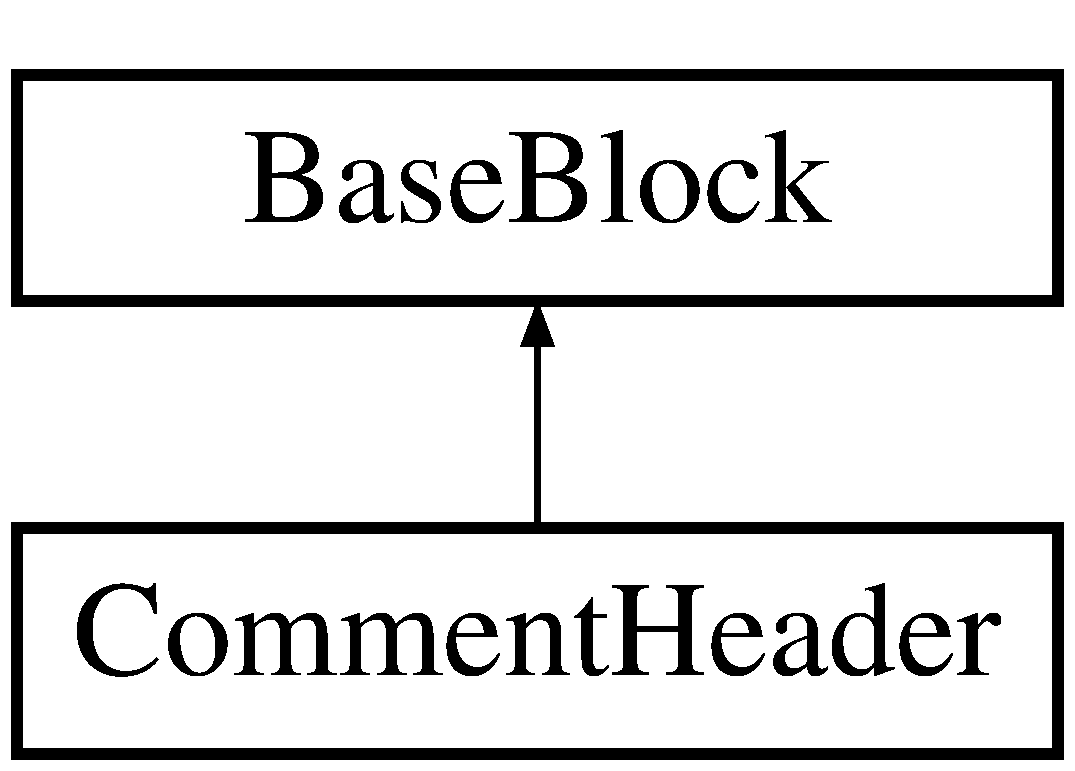
\includegraphics[height=2.000000cm]{struct_comment_header}
\end{center}
\end{figure}
\subsection*{Public Attributes}
\begin{DoxyCompactItemize}
\item 
\hypertarget{struct_comment_header_aa1aeb9b48fda8a62f77a029d89da999e}{ushort {\bfseries Unp\-Size}}\label{struct_comment_header_aa1aeb9b48fda8a62f77a029d89da999e}

\item 
\hypertarget{struct_comment_header_a22b98c54ed8a00ff62687609afd309a6}{byte {\bfseries Unp\-Ver}}\label{struct_comment_header_a22b98c54ed8a00ff62687609afd309a6}

\item 
\hypertarget{struct_comment_header_a8a64cbb117d6694293f498995de77714}{byte {\bfseries Method}}\label{struct_comment_header_a8a64cbb117d6694293f498995de77714}

\item 
\hypertarget{struct_comment_header_aa356eb0314083402ded788a5e8910ca8}{ushort {\bfseries Comm\-C\-R\-C}}\label{struct_comment_header_aa356eb0314083402ded788a5e8910ca8}

\end{DoxyCompactItemize}
\subsection*{Additional Inherited Members}


The documentation for this struct was generated from the following file\-:\begin{DoxyCompactItemize}
\item 
/\-Users/salazbr1/\-Documents/\-N\-P\-S/final\-\_\-unrarbulk\-\_\-extractor\-\_\-07-\/26-\/12/code/headers.\-hpp\end{DoxyCompactItemize}

\hypertarget{class_compr_data_i_o}{\section{Compr\-Data\-I\-O Class Reference}
\label{class_compr_data_i_o}\index{Compr\-Data\-I\-O@{Compr\-Data\-I\-O}}
}
\subsection*{Public Member Functions}
\begin{DoxyCompactItemize}
\item 
\hypertarget{class_compr_data_i_o_a9b34d7306fa75a0e41e0da0823e069c1}{void {\bfseries Init} ()}\label{class_compr_data_i_o_a9b34d7306fa75a0e41e0da0823e069c1}

\item 
\hypertarget{class_compr_data_i_o_a88d35dededb1d3f85245f78c65852404}{int {\bfseries Unp\-Read} (byte $\ast$Addr, size\-\_\-t Count)}\label{class_compr_data_i_o_a88d35dededb1d3f85245f78c65852404}

\item 
\hypertarget{class_compr_data_i_o_a2b4b6df672d70fd474a10bb67c0dac7e}{void {\bfseries Unp\-Write} (byte $\ast$Addr, size\-\_\-t Count)}\label{class_compr_data_i_o_a2b4b6df672d70fd474a10bb67c0dac7e}

\item 
\hypertarget{class_compr_data_i_o_a9d3adbdc2ef1b9178ef5ad8f1c02f33b}{void {\bfseries Enable\-Show\-Progress} (bool Show)}\label{class_compr_data_i_o_a9d3adbdc2ef1b9178ef5ad8f1c02f33b}

\item 
\hypertarget{class_compr_data_i_o_a957f3628403b4f5d4f568e2d3065e579}{void {\bfseries Get\-Unpacked\-Data} (byte $\ast$$\ast$Data, size\-\_\-t $\ast$Size)}\label{class_compr_data_i_o_a957f3628403b4f5d4f568e2d3065e579}

\item 
\hypertarget{class_compr_data_i_o_a9b10c1b9b500743d4cbbe4e2faa4a795}{void {\bfseries Set\-Packed\-Size\-To\-Read} (int64 Size)}\label{class_compr_data_i_o_a9b10c1b9b500743d4cbbe4e2faa4a795}

\item 
\hypertarget{class_compr_data_i_o_ac2f0c203f5c3fb342167709c9cc01072}{void {\bfseries Set\-Test\-Mode} (bool Mode)}\label{class_compr_data_i_o_ac2f0c203f5c3fb342167709c9cc01072}

\item 
\hypertarget{class_compr_data_i_o_a712adbd109666f36a45156ac5c646f6e}{void {\bfseries Set\-Skip\-Unp\-C\-R\-C} (bool Skip)}\label{class_compr_data_i_o_a712adbd109666f36a45156ac5c646f6e}

\item 
\hypertarget{class_compr_data_i_o_a9c219e2c7b6c221cde925808ba91ac29}{void {\bfseries Set\-Files} (\hyperlink{class_file}{File} $\ast$Src\-File, \hyperlink{class_file}{File} $\ast$Dest\-File)}\label{class_compr_data_i_o_a9c219e2c7b6c221cde925808ba91ac29}

\item 
\hypertarget{class_compr_data_i_o_a13f1a0006a814cffc12f637e4b9cd394}{void {\bfseries Set\-Command} (Cmd\-Add $\ast$Cmd)}\label{class_compr_data_i_o_a13f1a0006a814cffc12f637e4b9cd394}

\item 
\hypertarget{class_compr_data_i_o_ac668e4ab5228552d554ae25435ef28c2}{void {\bfseries Set\-Sub\-Header} (\hyperlink{struct_file_header}{File\-Header} $\ast$hd, int64 $\ast$Pos)}\label{class_compr_data_i_o_ac668e4ab5228552d554ae25435ef28c2}

\item 
\hypertarget{class_compr_data_i_o_af81b2fa4a0b74b5048307f11f0285bb8}{void {\bfseries Set\-Encryption} (int Method, const wchar $\ast$Password, const byte $\ast$Salt, bool Encrypt, bool Hands\-Off\-Hash)}\label{class_compr_data_i_o_af81b2fa4a0b74b5048307f11f0285bb8}

\item 
\hypertarget{class_compr_data_i_o_ae778fbef5bc6d99ae3985115083e9ec2}{void {\bfseries Set\-A\-V15\-Encryption} ()}\label{class_compr_data_i_o_ae778fbef5bc6d99ae3985115083e9ec2}

\item 
\hypertarget{class_compr_data_i_o_a248f726707d75e797e53ca148ccee020}{void {\bfseries Set\-Cmt13\-Encryption} ()}\label{class_compr_data_i_o_a248f726707d75e797e53ca148ccee020}

\item 
\hypertarget{class_compr_data_i_o_ae80811c83ce1bda80692abe6fd8c3d94}{void {\bfseries Set\-Unpack\-To\-Memory} (byte $\ast$Addr, uint Size)}\label{class_compr_data_i_o_ae80811c83ce1bda80692abe6fd8c3d94}

\item 
\hypertarget{class_compr_data_i_o_a4b071da90bf0de99fa656e174192cea1}{void {\bfseries Set\-Current\-Command} (char Cmd)}\label{class_compr_data_i_o_a4b071da90bf0de99fa656e174192cea1}

\end{DoxyCompactItemize}
\subsection*{Public Attributes}
\begin{DoxyCompactItemize}
\item 
\hypertarget{class_compr_data_i_o_a4dfd398f59279cfcd6c5d23898f4231e}{bool {\bfseries Pack\-Volume}}\label{class_compr_data_i_o_a4dfd398f59279cfcd6c5d23898f4231e}

\item 
\hypertarget{class_compr_data_i_o_a9b58563d6b9e6dafeaba103f60f3afc5}{bool {\bfseries Unp\-Volume}}\label{class_compr_data_i_o_a9b58563d6b9e6dafeaba103f60f3afc5}

\item 
\hypertarget{class_compr_data_i_o_a1077651f8e105e8287b5937c9fabd7af}{bool {\bfseries Next\-Volume\-Missing}}\label{class_compr_data_i_o_a1077651f8e105e8287b5937c9fabd7af}

\item 
\hypertarget{class_compr_data_i_o_a4af9ec517617dbd5b7a023bc1a5e2308}{int64 {\bfseries Total\-Pack\-Read}}\label{class_compr_data_i_o_a4af9ec517617dbd5b7a023bc1a5e2308}

\item 
\hypertarget{class_compr_data_i_o_abc1cf117c7f276bd046b905d5734fc8d}{int64 {\bfseries Unp\-Arc\-Size}}\label{class_compr_data_i_o_abc1cf117c7f276bd046b905d5734fc8d}

\item 
\hypertarget{class_compr_data_i_o_ad8ce53e55f113e957f098cd16d090509}{int64 {\bfseries Cur\-Pack\-Read}}\label{class_compr_data_i_o_ad8ce53e55f113e957f098cd16d090509}

\item 
\hypertarget{class_compr_data_i_o_a9a158db20dfc888dfeb0642f3240bf9f}{int64 {\bfseries Cur\-Pack\-Write}}\label{class_compr_data_i_o_a9a158db20dfc888dfeb0642f3240bf9f}

\item 
\hypertarget{class_compr_data_i_o_ac506412e9e677d88d4d97f4038a2924c}{int64 {\bfseries Cur\-Unp\-Read}}\label{class_compr_data_i_o_ac506412e9e677d88d4d97f4038a2924c}

\item 
\hypertarget{class_compr_data_i_o_a19011da165359d190a2da58e534afbed}{int64 {\bfseries Cur\-Unp\-Write}}\label{class_compr_data_i_o_a19011da165359d190a2da58e534afbed}

\item 
\hypertarget{class_compr_data_i_o_a4541b60af00a6a732093e701205a2f2c}{int64 {\bfseries Processed\-Arc\-Size}}\label{class_compr_data_i_o_a4541b60af00a6a732093e701205a2f2c}

\item 
\hypertarget{class_compr_data_i_o_a4714f96bf752047b51301ee8f03e9cca}{int64 {\bfseries Total\-Arc\-Size}}\label{class_compr_data_i_o_a4714f96bf752047b51301ee8f03e9cca}

\item 
\hypertarget{class_compr_data_i_o_aeb8b7ef01b466bbad70daf8ca86d864d}{uint {\bfseries Pack\-File\-C\-R\-C}}\label{class_compr_data_i_o_aeb8b7ef01b466bbad70daf8ca86d864d}

\item 
\hypertarget{class_compr_data_i_o_a44e7244fee333a0f1b03a4349b2189e0}{uint {\bfseries Unp\-File\-C\-R\-C}}\label{class_compr_data_i_o_a44e7244fee333a0f1b03a4349b2189e0}

\item 
\hypertarget{class_compr_data_i_o_a0b17289dab91eb5a33d40fae0b9ec325}{uint {\bfseries Packed\-C\-R\-C}}\label{class_compr_data_i_o_a0b17289dab91eb5a33d40fae0b9ec325}

\item 
\hypertarget{class_compr_data_i_o_a5fd109bfd8c6b25b54a9752a6976d1cf}{int {\bfseries Encryption}}\label{class_compr_data_i_o_a5fd109bfd8c6b25b54a9752a6976d1cf}

\item 
\hypertarget{class_compr_data_i_o_a681245c58c7f46d56575f63e0d994492}{int {\bfseries Decryption}}\label{class_compr_data_i_o_a681245c58c7f46d56575f63e0d994492}

\end{DoxyCompactItemize}


The documentation for this class was generated from the following files\-:\begin{DoxyCompactItemize}
\item 
/\-Users/salazbr1/\-Documents/\-N\-P\-S/final\-\_\-unrarbulk\-\_\-extractor\-\_\-07-\/26-\/12/code/rdwrfn.\-hpp\item 
/\-Users/salazbr1/\-Documents/\-N\-P\-S/final\-\_\-unrarbulk\-\_\-extractor\-\_\-07-\/26-\/12/code/rdwrfn.\-cpp\end{DoxyCompactItemize}

\hypertarget{class_crypt_data}{\section{Crypt\-Data Class Reference}
\label{class_crypt_data}\index{Crypt\-Data@{Crypt\-Data}}
}
\subsection*{Public Member Functions}
\begin{DoxyCompactItemize}
\item 
\hypertarget{class_crypt_data_ad966dfc927aeeb20c6f2d7282bb49c55}{void {\bfseries Set\-Crypt\-Keys} (const wchar $\ast$Password, const byte $\ast$Salt, bool Encrypt, bool Old\-Only, bool Hands\-Off\-Hash)}\label{class_crypt_data_ad966dfc927aeeb20c6f2d7282bb49c55}

\item 
\hypertarget{class_crypt_data_acea183e5b27efea3dfcc6fe0a1f8c71b}{void {\bfseries Set\-A\-V15\-Encryption} ()}\label{class_crypt_data_acea183e5b27efea3dfcc6fe0a1f8c71b}

\item 
\hypertarget{class_crypt_data_a86c0d7a539a508a4d9dd5cbeb5a22c09}{void {\bfseries Set\-Cmt13\-Encryption} ()}\label{class_crypt_data_a86c0d7a539a508a4d9dd5cbeb5a22c09}

\item 
\hypertarget{class_crypt_data_a04331297a6175bba2b0115b0b5db948d}{void {\bfseries Encrypt\-Block20} (byte $\ast$Buf)}\label{class_crypt_data_a04331297a6175bba2b0115b0b5db948d}

\item 
\hypertarget{class_crypt_data_adcb3af7e7771ef28856f1e0de5d449c2}{void {\bfseries Decrypt\-Block20} (byte $\ast$Buf)}\label{class_crypt_data_adcb3af7e7771ef28856f1e0de5d449c2}

\item 
\hypertarget{class_crypt_data_aa66eb131f5babe624563c7958c0d9d0c}{void {\bfseries Encrypt\-Block} (byte $\ast$Buf, size\-\_\-t Size)}\label{class_crypt_data_aa66eb131f5babe624563c7958c0d9d0c}

\item 
\hypertarget{class_crypt_data_adfd78aeb9b855fcfb8eeb77c99732771}{void {\bfseries Decrypt\-Block} (byte $\ast$Buf, size\-\_\-t Size)}\label{class_crypt_data_adfd78aeb9b855fcfb8eeb77c99732771}

\item 
\hypertarget{class_crypt_data_ab8fa43a011aaf809eb3193fa4295124b}{void {\bfseries Crypt} (byte $\ast$Data, uint Count, int Method)}\label{class_crypt_data_ab8fa43a011aaf809eb3193fa4295124b}

\end{DoxyCompactItemize}
\subsection*{Static Public Member Functions}
\begin{DoxyCompactItemize}
\item 
\hypertarget{class_crypt_data_a8ec5054ba51bf5d94d81a92dd2213134}{static void {\bfseries Set\-Salt} (byte $\ast$Salt, int Salt\-Size)}\label{class_crypt_data_a8ec5054ba51bf5d94d81a92dd2213134}

\end{DoxyCompactItemize}


The documentation for this class was generated from the following files\-:\begin{DoxyCompactItemize}
\item 
/\-Users/salazbr1/\-Documents/\-N\-P\-S/final\-\_\-unrarbulk\-\_\-extractor\-\_\-07-\/26-\/12/code/crypt.\-hpp\item 
/\-Users/salazbr1/\-Documents/\-N\-P\-S/final\-\_\-unrarbulk\-\_\-extractor\-\_\-07-\/26-\/12/code/crypt.\-cpp\end{DoxyCompactItemize}

\hypertarget{struct_crypt_key_cache_item}{\section{Crypt\-Key\-Cache\-Item Struct Reference}
\label{struct_crypt_key_cache_item}\index{Crypt\-Key\-Cache\-Item@{Crypt\-Key\-Cache\-Item}}
}
\subsection*{Public Attributes}
\begin{DoxyCompactItemize}
\item 
\hypertarget{struct_crypt_key_cache_item_a766794c91064e89b1ce20749ad577392}{byte {\bfseries A\-E\-S\-Key} \mbox{[}16\mbox{]}}\label{struct_crypt_key_cache_item_a766794c91064e89b1ce20749ad577392}

\item 
\hypertarget{struct_crypt_key_cache_item_a91843c1ca6dbee6fbaed31d2edeaf9f7}{byte {\bfseries A\-E\-S\-Init} \mbox{[}16\mbox{]}}\label{struct_crypt_key_cache_item_a91843c1ca6dbee6fbaed31d2edeaf9f7}

\item 
\hypertarget{struct_crypt_key_cache_item_a71d480efb1c3c0258fe97e659c57edd8}{wchar {\bfseries Password} \mbox{[}M\-A\-X\-P\-A\-S\-S\-W\-O\-R\-D\mbox{]}}\label{struct_crypt_key_cache_item_a71d480efb1c3c0258fe97e659c57edd8}

\item 
\hypertarget{struct_crypt_key_cache_item_a959682f1e006bbfadf6dc1f8d628ef6a}{bool {\bfseries Salt\-Present}}\label{struct_crypt_key_cache_item_a959682f1e006bbfadf6dc1f8d628ef6a}

\item 
\hypertarget{struct_crypt_key_cache_item_adfbaf4a6733f70f4e6add54e40d85a3a}{byte {\bfseries Salt} \mbox{[}S\-A\-L\-T\-\_\-\-S\-I\-Z\-E\mbox{]}}\label{struct_crypt_key_cache_item_adfbaf4a6733f70f4e6add54e40d85a3a}

\item 
\hypertarget{struct_crypt_key_cache_item_a4f99eebd37130aba807b69a014f0abf9}{bool {\bfseries Hands\-Off\-Hash}}\label{struct_crypt_key_cache_item_a4f99eebd37130aba807b69a014f0abf9}

\end{DoxyCompactItemize}


The documentation for this struct was generated from the following file\-:\begin{DoxyCompactItemize}
\item 
/\-Users/salazbr1/\-Documents/\-N\-P\-S/final\-\_\-unrarbulk\-\_\-extractor\-\_\-07-\/26-\/12/code/crypt.\-hpp\end{DoxyCompactItemize}

\hypertarget{struct_data_set}{\section{Data\-Set Struct Reference}
\label{struct_data_set}\index{Data\-Set@{Data\-Set}}
}
\subsection*{Public Attributes}
\begin{DoxyCompactItemize}
\item 
\hypertarget{struct_data_set_afa8cc4d545dd6096f7bc1c405940df33}{\hyperlink{class_command_data}{Command\-Data} {\bfseries Cmd}}\label{struct_data_set_afa8cc4d545dd6096f7bc1c405940df33}

\item 
\hypertarget{struct_data_set_aa44e543420917338ddf434a0f031302f}{\hyperlink{class_cmd_extract}{Cmd\-Extract} {\bfseries Extract}}\label{struct_data_set_aa44e543420917338ddf434a0f031302f}

\item 
\hypertarget{struct_data_set_a9d63ec4ab19d8657b441a46c40712345}{\hyperlink{class_archive}{Archive} {\bfseries Arc}}\label{struct_data_set_a9d63ec4ab19d8657b441a46c40712345}

\item 
\hypertarget{struct_data_set_a899cc829146adf2907aff0fba4dfd435}{int {\bfseries Open\-Mode}}\label{struct_data_set_a899cc829146adf2907aff0fba4dfd435}

\item 
\hypertarget{struct_data_set_afff4c9b6ad3d80f1caf5a5db7cb2c05f}{int {\bfseries Header\-Size}}\label{struct_data_set_afff4c9b6ad3d80f1caf5a5db7cb2c05f}

\end{DoxyCompactItemize}


The documentation for this struct was generated from the following file\-:\begin{DoxyCompactItemize}
\item 
/\-Users/salazbr1/\-Documents/\-N\-P\-S/final\-\_\-unrarbulk\-\_\-extractor\-\_\-07-\/26-\/12/code/dll.\-cpp\end{DoxyCompactItemize}

\hypertarget{struct_decode_table}{\section{Decode\-Table Struct Reference}
\label{struct_decode_table}\index{Decode\-Table@{Decode\-Table}}
}
\subsection*{Public Attributes}
\begin{DoxyCompactItemize}
\item 
\hypertarget{struct_decode_table_a3c8068ab36d6da313ead79119fdd162c}{uint {\bfseries Max\-Num}}\label{struct_decode_table_a3c8068ab36d6da313ead79119fdd162c}

\item 
\hypertarget{struct_decode_table_ade30adc229dd1c26d1883d2b5877461e}{uint {\bfseries Decode\-Len} \mbox{[}16\mbox{]}}\label{struct_decode_table_ade30adc229dd1c26d1883d2b5877461e}

\item 
\hypertarget{struct_decode_table_a813fb62e2aa373b95c948eb7e7214e7d}{uint {\bfseries Decode\-Pos} \mbox{[}16\mbox{]}}\label{struct_decode_table_a813fb62e2aa373b95c948eb7e7214e7d}

\item 
\hypertarget{struct_decode_table_a5688b194310750e7828a4430fd3dc6a7}{uint {\bfseries Quick\-Bits}}\label{struct_decode_table_a5688b194310750e7828a4430fd3dc6a7}

\item 
\hypertarget{struct_decode_table_a4abf7a8bb6d54688bc8ba67c0a609174}{byte {\bfseries Quick\-Len} \mbox{[}1$<$$<$ M\-A\-X\-\_\-\-Q\-U\-I\-C\-K\-\_\-\-D\-E\-C\-O\-D\-E\-\_\-\-B\-I\-T\-S\mbox{]}}\label{struct_decode_table_a4abf7a8bb6d54688bc8ba67c0a609174}

\item 
\hypertarget{struct_decode_table_adab0e0cd077022f81a0a10b2f5f3fe88}{uint {\bfseries Quick\-Num} \mbox{[}1$<$$<$ M\-A\-X\-\_\-\-Q\-U\-I\-C\-K\-\_\-\-D\-E\-C\-O\-D\-E\-\_\-\-B\-I\-T\-S\mbox{]}}\label{struct_decode_table_adab0e0cd077022f81a0a10b2f5f3fe88}

\item 
\hypertarget{struct_decode_table_aeaa83ba1918c7574968b400de91b3e6a}{uint {\bfseries Decode\-Num} \mbox{[}L\-A\-R\-G\-E\-S\-T\-\_\-\-T\-A\-B\-L\-E\-\_\-\-S\-I\-Z\-E\mbox{]}}\label{struct_decode_table_aeaa83ba1918c7574968b400de91b3e6a}

\end{DoxyCompactItemize}


The documentation for this struct was generated from the following file\-:\begin{DoxyCompactItemize}
\item 
/\-Users/salazbr1/\-Documents/\-N\-P\-S/final\-\_\-unrarbulk\-\_\-extractor\-\_\-07-\/26-\/12/code/unpack.\-hpp\end{DoxyCompactItemize}

\hypertarget{struct_e_a_header}{\section{E\-A\-Header Struct Reference}
\label{struct_e_a_header}\index{E\-A\-Header@{E\-A\-Header}}
}
Inheritance diagram for E\-A\-Header\-:\begin{figure}[H]
\begin{center}
\leavevmode
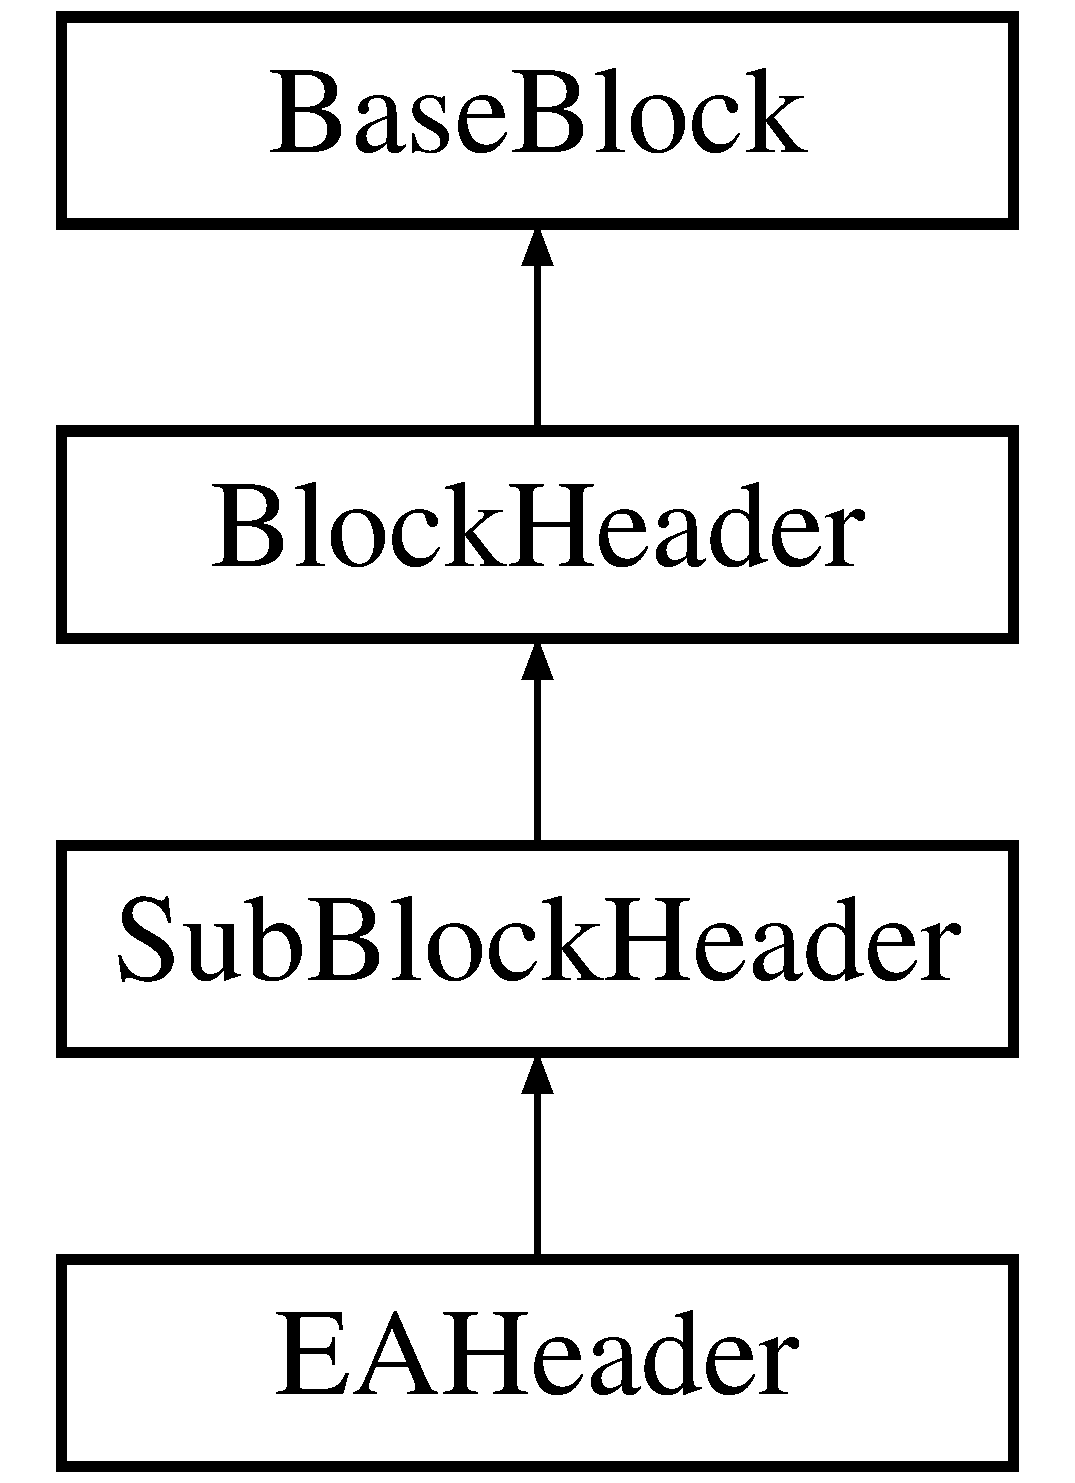
\includegraphics[height=4.000000cm]{struct_e_a_header}
\end{center}
\end{figure}
\subsection*{Public Attributes}
\begin{DoxyCompactItemize}
\item 
\hypertarget{struct_e_a_header_a9d53720536c4f83e263f3a97bca23ed8}{uint {\bfseries Unp\-Size}}\label{struct_e_a_header_a9d53720536c4f83e263f3a97bca23ed8}

\item 
\hypertarget{struct_e_a_header_acc8d60390806f2b38eec17b6756e7114}{byte {\bfseries Unp\-Ver}}\label{struct_e_a_header_acc8d60390806f2b38eec17b6756e7114}

\item 
\hypertarget{struct_e_a_header_a1529ecbae7f5881e779645758675ebac}{byte {\bfseries Method}}\label{struct_e_a_header_a1529ecbae7f5881e779645758675ebac}

\item 
\hypertarget{struct_e_a_header_ab58cbf18b6ca3620ed8bd4196edc0769}{uint {\bfseries E\-A\-C\-R\-C}}\label{struct_e_a_header_ab58cbf18b6ca3620ed8bd4196edc0769}

\end{DoxyCompactItemize}


The documentation for this struct was generated from the following file\-:\begin{DoxyCompactItemize}
\item 
/\-Users/salazbr1/\-Documents/\-N\-P\-S/final\-\_\-unrarbulk\-\_\-extractor\-\_\-07-\/26-\/12/code/headers.\-hpp\end{DoxyCompactItemize}

\hypertarget{class_encode_file_name}{\section{Encode\-File\-Name Class Reference}
\label{class_encode_file_name}\index{Encode\-File\-Name@{Encode\-File\-Name}}
}
\subsection*{Public Member Functions}
\begin{DoxyCompactItemize}
\item 
\hypertarget{class_encode_file_name_a7b8d0b197bd1e947f7a81f5a06155e5a}{size\-\_\-t {\bfseries Encode} (char $\ast$Name, wchar $\ast$Name\-W, byte $\ast$Enc\-Name)}\label{class_encode_file_name_a7b8d0b197bd1e947f7a81f5a06155e5a}

\item 
\hypertarget{class_encode_file_name_a87e52ed229f07719dd9d78e09c10cf5c}{void {\bfseries Decode} (char $\ast$Name, byte $\ast$Enc\-Name, size\-\_\-t Enc\-Size, wchar $\ast$Name\-W, size\-\_\-t Max\-Dec\-Size)}\label{class_encode_file_name_a87e52ed229f07719dd9d78e09c10cf5c}

\end{DoxyCompactItemize}


The documentation for this class was generated from the following files\-:\begin{DoxyCompactItemize}
\item 
/\-Users/salazbr1/\-Documents/\-N\-P\-S/final\-\_\-unrarbulk\-\_\-extractor\-\_\-07-\/26-\/12/code/encname.\-hpp\item 
/\-Users/salazbr1/\-Documents/\-N\-P\-S/final\-\_\-unrarbulk\-\_\-extractor\-\_\-07-\/26-\/12/code/encname.\-cpp\end{DoxyCompactItemize}

\hypertarget{struct_end_arc_header}{\section{End\-Arc\-Header Struct Reference}
\label{struct_end_arc_header}\index{End\-Arc\-Header@{End\-Arc\-Header}}
}
Inheritance diagram for End\-Arc\-Header\-:\begin{figure}[H]
\begin{center}
\leavevmode
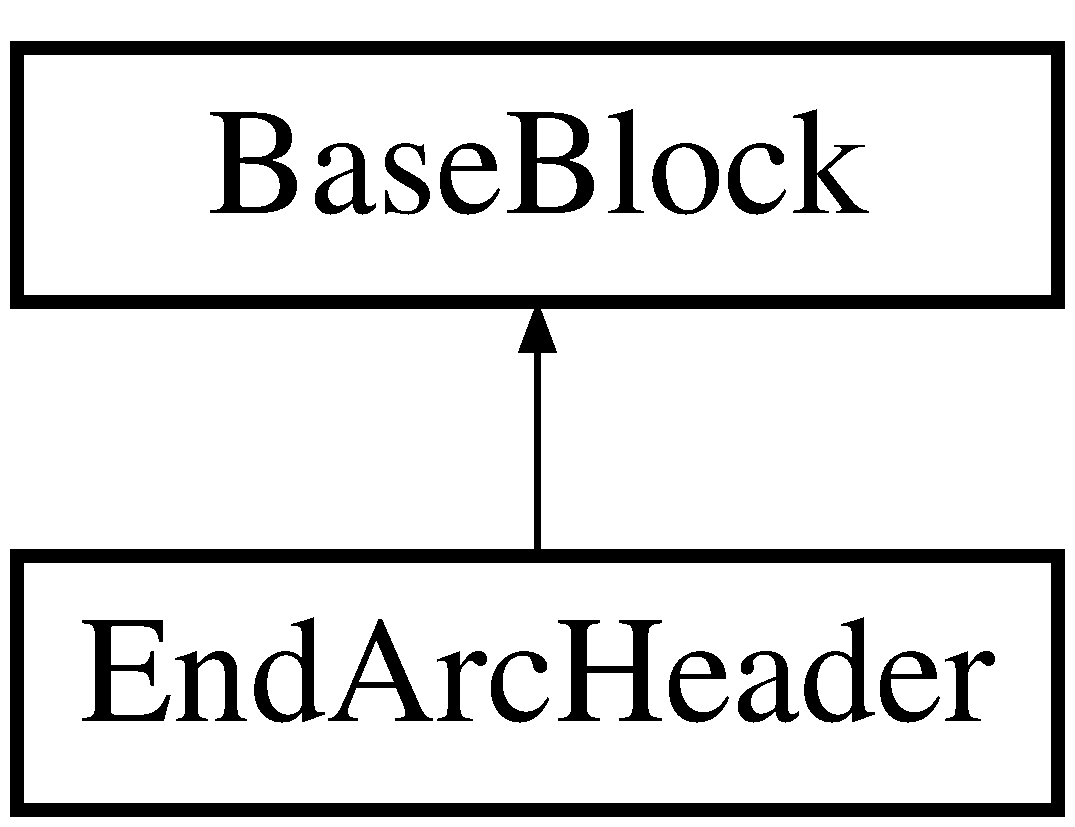
\includegraphics[height=2.000000cm]{struct_end_arc_header}
\end{center}
\end{figure}
\subsection*{Public Attributes}
\begin{DoxyCompactItemize}
\item 
\hypertarget{struct_end_arc_header_a7312da8b7a708fe45b5ab6d13b631233}{uint {\bfseries Arc\-Data\-C\-R\-C}}\label{struct_end_arc_header_a7312da8b7a708fe45b5ab6d13b631233}

\item 
\hypertarget{struct_end_arc_header_a46ea67c6ccd96313761d9941b62e3899}{ushort {\bfseries Vol\-Number}}\label{struct_end_arc_header_a46ea67c6ccd96313761d9941b62e3899}

\end{DoxyCompactItemize}
\subsection*{Additional Inherited Members}


The documentation for this struct was generated from the following file\-:\begin{DoxyCompactItemize}
\item 
/\-Users/salazbr1/\-Documents/\-N\-P\-S/final\-\_\-unrarbulk\-\_\-extractor\-\_\-07-\/26-\/12/code/headers.\-hpp\end{DoxyCompactItemize}

\hypertarget{class_error_handler}{\section{Error\-Handler Class Reference}
\label{class_error_handler}\index{Error\-Handler@{Error\-Handler}}
}
\subsection*{Public Member Functions}
\begin{DoxyCompactItemize}
\item 
\hypertarget{class_error_handler_aafe35f48d34a8dcda3801a7bef24595d}{void {\bfseries Clean} ()}\label{class_error_handler_aafe35f48d34a8dcda3801a7bef24595d}

\item 
\hypertarget{class_error_handler_ab8a639bac5170654821838d8cb278f2c}{void {\bfseries Memory\-Error} ()}\label{class_error_handler_ab8a639bac5170654821838d8cb278f2c}

\item 
\hypertarget{class_error_handler_a0fcf5384291154219b75d0c21b29fd96}{void {\bfseries Open\-Error} (const char $\ast$File\-Name, const wchar $\ast$File\-Name\-W)}\label{class_error_handler_a0fcf5384291154219b75d0c21b29fd96}

\item 
\hypertarget{class_error_handler_af8e2a28d2dc2532b5a9a28becaf82d9a}{void {\bfseries Close\-Error} (const char $\ast$File\-Name, const wchar $\ast$File\-Name\-W)}\label{class_error_handler_af8e2a28d2dc2532b5a9a28becaf82d9a}

\item 
\hypertarget{class_error_handler_a7009ffd4d1038588dd15d9c1837d530c}{void {\bfseries Read\-Error} (const char $\ast$File\-Name, const wchar $\ast$File\-Name\-W)}\label{class_error_handler_a7009ffd4d1038588dd15d9c1837d530c}

\item 
\hypertarget{class_error_handler_a326e8eddaf1a6d9f0ee0f5c1964f89a6}{bool {\bfseries Ask\-Repeat\-Read} (const char $\ast$File\-Name, const wchar $\ast$File\-Name\-W)}\label{class_error_handler_a326e8eddaf1a6d9f0ee0f5c1964f89a6}

\item 
\hypertarget{class_error_handler_abf5299128386cbaec6bff11ce0d54c31}{void {\bfseries Write\-Error} (const char $\ast$Arc\-Name, const wchar $\ast$Arc\-Name\-W, const char $\ast$File\-Name, const wchar $\ast$File\-Name\-W)}\label{class_error_handler_abf5299128386cbaec6bff11ce0d54c31}

\item 
\hypertarget{class_error_handler_ac3b7d29de62895ee52f0418be18baa38}{void {\bfseries Write\-Error\-F\-A\-T} (const char $\ast$File\-Name, const wchar $\ast$File\-Name\-W)}\label{class_error_handler_ac3b7d29de62895ee52f0418be18baa38}

\item 
\hypertarget{class_error_handler_ace50152e9951ace7d7282fa977af370f}{bool {\bfseries Ask\-Repeat\-Write} (const char $\ast$File\-Name, const wchar $\ast$File\-Name\-W, bool Disk\-Full)}\label{class_error_handler_ace50152e9951ace7d7282fa977af370f}

\item 
\hypertarget{class_error_handler_aba3505f65f04e88336a8ee928fc418fe}{void {\bfseries Seek\-Error} (const char $\ast$File\-Name, const wchar $\ast$File\-Name\-W)}\label{class_error_handler_aba3505f65f04e88336a8ee928fc418fe}

\item 
\hypertarget{class_error_handler_a9007bfe9f6fcd70afaf01bb058af96f8}{void {\bfseries General\-Err\-Msg} (const char $\ast$Msg)}\label{class_error_handler_a9007bfe9f6fcd70afaf01bb058af96f8}

\item 
\hypertarget{class_error_handler_a1bec4ce4887d2fe7de76aec3157efcfb}{void {\bfseries Memory\-Error\-Msg} ()}\label{class_error_handler_a1bec4ce4887d2fe7de76aec3157efcfb}

\item 
\hypertarget{class_error_handler_a488606304d3f4c48e92812c1d48e5aee}{void {\bfseries Open\-Error\-Msg} (const char $\ast$File\-Name, const wchar $\ast$File\-Name\-W=N\-U\-L\-L)}\label{class_error_handler_a488606304d3f4c48e92812c1d48e5aee}

\item 
\hypertarget{class_error_handler_af74f303e2d9bfd16f13a1dc02c4bb637}{void {\bfseries Open\-Error\-Msg} (const char $\ast$Arc\-Name, const wchar $\ast$Arc\-Name\-W, const char $\ast$File\-Name, const wchar $\ast$File\-Name\-W)}\label{class_error_handler_af74f303e2d9bfd16f13a1dc02c4bb637}

\item 
\hypertarget{class_error_handler_ac7aabf8de9a2a5e21286a61755842aba}{void {\bfseries Create\-Error\-Msg} (const char $\ast$File\-Name, const wchar $\ast$File\-Name\-W=N\-U\-L\-L)}\label{class_error_handler_ac7aabf8de9a2a5e21286a61755842aba}

\item 
\hypertarget{class_error_handler_a50edd97c4397064bf09ff30eea7e1e0c}{void {\bfseries Create\-Error\-Msg} (const char $\ast$Arc\-Name, const wchar $\ast$Arc\-Name\-W, const char $\ast$File\-Name, const wchar $\ast$File\-Name\-W)}\label{class_error_handler_a50edd97c4397064bf09ff30eea7e1e0c}

\item 
\hypertarget{class_error_handler_aeeeb484b88af6f8911ea537fba35ac54}{void {\bfseries Check\-Long\-Path\-Err\-Msg} (const char $\ast$File\-Name, const wchar $\ast$File\-Name\-W)}\label{class_error_handler_aeeeb484b88af6f8911ea537fba35ac54}

\item 
\hypertarget{class_error_handler_af808d21777b932172c0f5808b074e6fc}{void {\bfseries Read\-Error\-Msg} (const char $\ast$Arc\-Name, const wchar $\ast$Arc\-Name\-W, const char $\ast$File\-Name, const wchar $\ast$File\-Name\-W)}\label{class_error_handler_af808d21777b932172c0f5808b074e6fc}

\item 
\hypertarget{class_error_handler_ade8b41d944a3c8291bcdc647c59ef8e4}{void {\bfseries Write\-Error\-Msg} (const char $\ast$Arc\-Name, const wchar $\ast$Arc\-Name\-W, const char $\ast$File\-Name, const wchar $\ast$File\-Name\-W)}\label{class_error_handler_ade8b41d944a3c8291bcdc647c59ef8e4}

\item 
\hypertarget{class_error_handler_ab4df1a5a4550a6c8afebb6d6631439b0}{void {\bfseries Exit} (int Exit\-Code)}\label{class_error_handler_ab4df1a5a4550a6c8afebb6d6631439b0}

\item 
\hypertarget{class_error_handler_a12a27859f5b079ee7cf18713d6abda4e}{void {\bfseries Set\-Error\-Code} (int Code)}\label{class_error_handler_a12a27859f5b079ee7cf18713d6abda4e}

\item 
\hypertarget{class_error_handler_a04b649c09b0a16861b3b4c7d0170c277}{int {\bfseries Get\-Error\-Code} ()}\label{class_error_handler_a04b649c09b0a16861b3b4c7d0170c277}

\item 
\hypertarget{class_error_handler_a82f5fc590a7a0e7f806f2372d842db39}{int {\bfseries Get\-Error\-Count} ()}\label{class_error_handler_a82f5fc590a7a0e7f806f2372d842db39}

\item 
\hypertarget{class_error_handler_a68b0990729a2f4fa40ed26e19cfe1d40}{void {\bfseries Set\-Signal\-Handlers} (bool Enable)}\label{class_error_handler_a68b0990729a2f4fa40ed26e19cfe1d40}

\item 
\hypertarget{class_error_handler_a275bc9640f6927bc491df82c5219f147}{void {\bfseries Throw} (int Code)}\label{class_error_handler_a275bc9640f6927bc491df82c5219f147}

\item 
\hypertarget{class_error_handler_aa2d17e2b29bc34a506b1c120774b584c}{void {\bfseries Set\-Silent} (bool Mode)}\label{class_error_handler_aa2d17e2b29bc34a506b1c120774b584c}

\item 
\hypertarget{class_error_handler_a150129e132207aaeedb1c0918526138e}{void {\bfseries Set\-Shutdown} (bool Mode)}\label{class_error_handler_a150129e132207aaeedb1c0918526138e}

\item 
\hypertarget{class_error_handler_a4c79a149a5fd10ed3989c20ac501c1d9}{void {\bfseries Sys\-Err\-Msg} ()}\label{class_error_handler_a4c79a149a5fd10ed3989c20ac501c1d9}

\end{DoxyCompactItemize}


The documentation for this class was generated from the following files\-:\begin{DoxyCompactItemize}
\item 
/\-Users/salazbr1/\-Documents/\-N\-P\-S/final\-\_\-unrarbulk\-\_\-extractor\-\_\-07-\/26-\/12/code/errhnd.\-hpp\item 
/\-Users/salazbr1/\-Documents/\-N\-P\-S/final\-\_\-unrarbulk\-\_\-extractor\-\_\-07-\/26-\/12/code/errhnd.\-cpp\end{DoxyCompactItemize}

\hypertarget{class_file}{\section{File Class Reference}
\label{class_file}\index{File@{File}}
}


{\ttfamily \#include $<$file.\-hpp$>$}

Inheritance diagram for File\-:\begin{figure}[H]
\begin{center}
\leavevmode
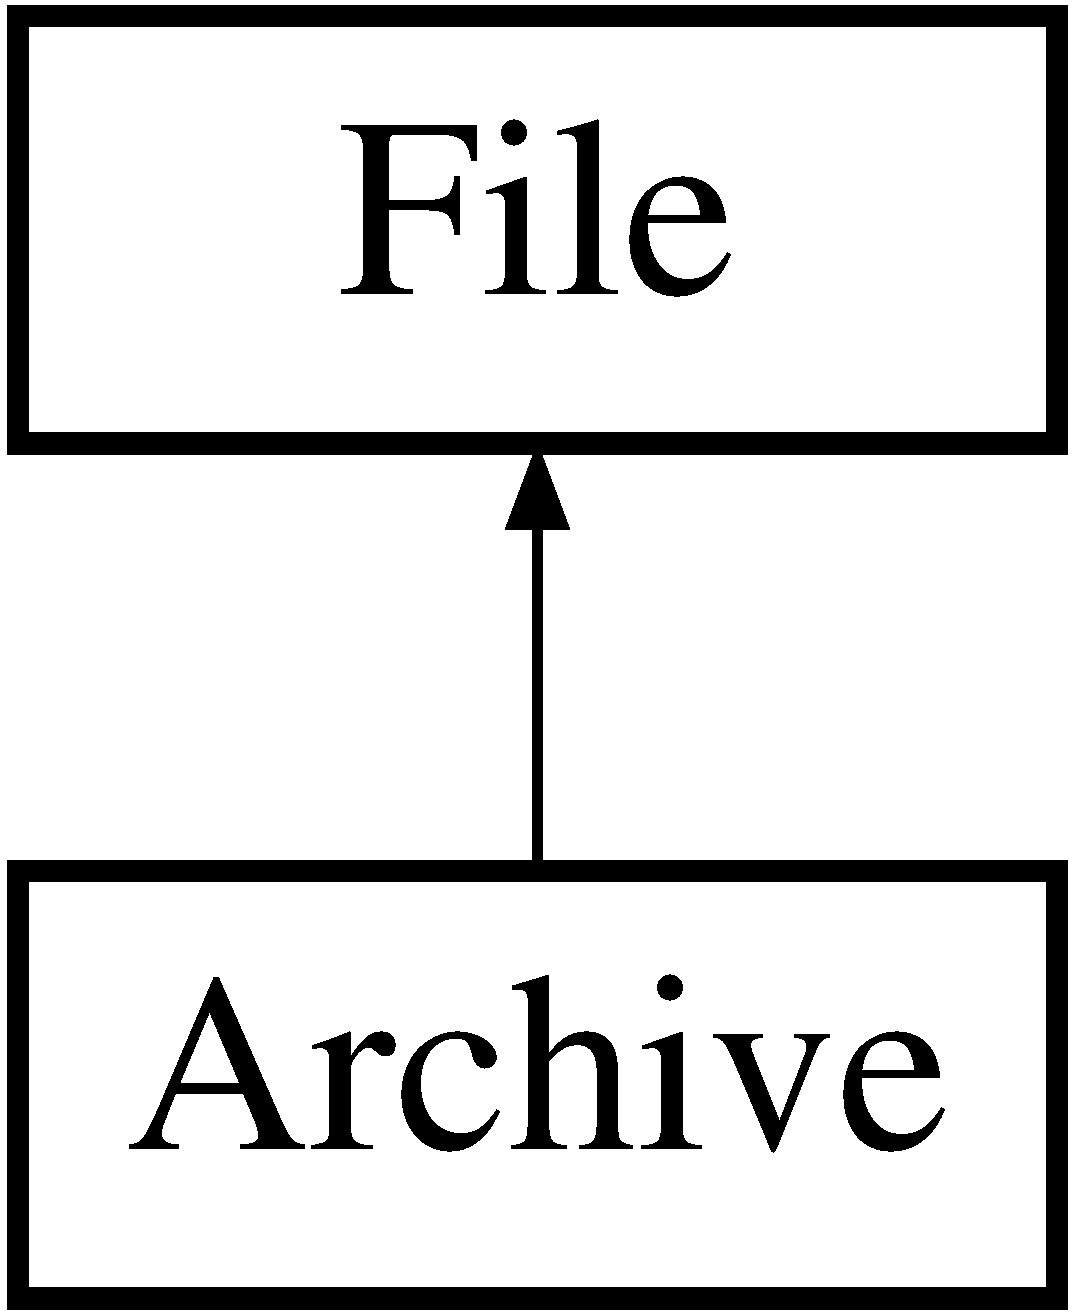
\includegraphics[height=2.000000cm]{class_file}
\end{center}
\end{figure}
\subsection*{Public Member Functions}
\begin{DoxyCompactItemize}
\item 
\hyperlink{class_file_ae039af5807fc385f41b60644725d15d0}{File} ()
\item 
void \hyperlink{class_file_ad25e907c17d68a3c0b72767a0390c500}{Init\-File} (void $\ast$ptr, int64 ptrlength)
\item 
void \hyperlink{class_file_af9b1f4f397084898a59a34fed18dad26}{operator=} (\hyperlink{class_file}{File} \&Src\-File)
\item 
\hypertarget{class_file_a705794d712d3425858778944004642a5}{bool {\bfseries Open} (const char $\ast$Name, const wchar $\ast$Name\-W=N\-U\-L\-L, bool Open\-Shared=false, bool Update=false)}\label{class_file_a705794d712d3425858778944004642a5}

\item 
void \hyperlink{class_file_a4d81ac5c1550fb1d45991bbaafc6d9a0}{T\-Open} (const char $\ast$Name, const wchar $\ast$Name\-W=N\-U\-L\-L)
\item 
bool \hyperlink{class_file_a6a4dead88fb112c2641fda5e4fa51f6f}{W\-Open} (const char $\ast$Name, const wchar $\ast$Name\-W=N\-U\-L\-L)
\item 
bool \hyperlink{class_file_a42b103889446cad09667c89d5ab0c323}{Create} (const char $\ast$Name, const wchar $\ast$Name\-W=N\-U\-L\-L, bool Share\-Read=true)
\item 
void \hyperlink{class_file_a4e9197e56f2c2fb669afe6713731734d}{T\-Create} (const char $\ast$Name, const wchar $\ast$Name\-W=N\-U\-L\-L, bool Share\-Read=true)
\item 
bool \hyperlink{class_file_a535a061342fa0814c3353bb9325fe0f4}{W\-Create} (const char $\ast$Name, const wchar $\ast$Name\-W=N\-U\-L\-L, bool Share\-Read=true)
\item 
bool \hyperlink{class_file_ad7ab440b2fba02aa291ecf5a00de8b8d}{Close} ()
\item 
void \hyperlink{class_file_a2791da7f792dcc2afb74eb6be78ab76b}{Flush} ()
\item 
bool \hyperlink{class_file_a840551732a156ad90a8d652d7b873402}{Delete} ()
\item 
bool \hyperlink{class_file_ad3fc3b622573a504300edc24a99003da}{Rename} (const char $\ast$New\-Name, const wchar $\ast$New\-Name\-W=N\-U\-L\-L)
\item 
void \hyperlink{class_file_aec61d0eefe6050f0c99fd25d4b7826a2}{Write} (const void $\ast$Data, size\-\_\-t Size)
\item 
int \hyperlink{class_file_a5744d4b49a30149b9e883d4cde735a01}{Read} (void $\ast$Data, size\-\_\-t Size)
\item 
int \hyperlink{class_file_add3a1b7186687db6e6ad1558b2f60efd}{Direct\-Read} (void $\ast$Data, size\-\_\-t Size)
\item 
int \hyperlink{class_file_ac17100017024ec51242e7502bc4e4472}{Direct\-Read} (byte $\ast$Data, size\-\_\-t Size)
\item 
void \hyperlink{class_file_a06c0ae1420585ff1c02c4755f4092e05}{Seek} (int64 Offset, int Method)
\item 
bool \hyperlink{class_file_adee143daa7c38172c7d84c7e7300b164}{Raw\-Seek} (int64 Offset, int Method)
\item 
int64 \hyperlink{class_file_a9613c522a3ec6a60d26b5b0c249857ec}{Tell} ()
\item 
int64 \hyperlink{class_file_a7d6bd1c7ef4aaf604c2c59726808d788}{Tell} (byte $\ast$addr)
\item 
void \hyperlink{class_file_ab331732c99a00a354ed5d9a66fe8d983}{Prealloc} (int64 Size)
\item 
byte \hyperlink{class_file_ab39c8afa7990da061eaf78bc892e2569}{Get\-Byte} ()
\item 
void \hyperlink{class_file_a46767ab04ecc36e9e841196ff00ed739}{Put\-Byte} (byte Byte)
\item 
bool \hyperlink{class_file_a0efa6caf9619e65a1d0cc431a03d4aa1}{Truncate} ()
\item 
void \hyperlink{class_file_aa63b65699e48434f94d8262d063fc408}{Set\-Open\-File\-Time} (\hyperlink{class_rar_time}{Rar\-Time} $\ast$ftm, \hyperlink{class_rar_time}{Rar\-Time} $\ast$ftc=N\-U\-L\-L, \hyperlink{class_rar_time}{Rar\-Time} $\ast$fta=N\-U\-L\-L)
\item 
void \hyperlink{class_file_a6a77f5d63a5f5aeee1a404803d50c2e1}{Set\-Close\-File\-Time} (\hyperlink{class_rar_time}{Rar\-Time} $\ast$ftm, \hyperlink{class_rar_time}{Rar\-Time} $\ast$fta=N\-U\-L\-L)
\item 
void \hyperlink{class_file_a230eb360fb1fc3223cf15f13f7a9b33f}{Get\-Open\-File\-Time} (\hyperlink{class_rar_time}{Rar\-Time} $\ast$ft)
\item 
\hypertarget{class_file_afdbf269bc408846178672dceef1b2b64}{bool {\bfseries Is\-Opened} ()}\label{class_file_afdbf269bc408846178672dceef1b2b64}

\item 
int64 \hyperlink{class_file_a2eca8a1052e0c5ade1bd04c337fbb539}{File\-Length} ()
\item 
void \hyperlink{class_file_a168c8cc895ab015d5afa4e66ba2b1515}{Set\-Handle\-Type} (F\-I\-L\-E\-\_\-\-H\-A\-N\-D\-L\-E\-T\-Y\-P\-E Type)
\item 
\hypertarget{class_file_a8be4cf189695c60e8104a6d983383fa6}{F\-I\-L\-E\-\_\-\-H\-A\-N\-D\-L\-E\-T\-Y\-P\-E {\bfseries Get\-Handle\-Type} ()}\label{class_file_a8be4cf189695c60e8104a6d983383fa6}

\item 
bool \hyperlink{class_file_a82de52af3430e61380868d0a88d19a43}{Is\-Device} ()
\item 
void \hyperlink{class_file_a0573c92d21fca7ef9d223bf5ee1e4e39}{fprintf} (const char $\ast$fmt,...)
\item 
\hypertarget{class_file_ae86874ceabe5161fa90e6d66888d73c1}{File\-Handle {\bfseries Get\-Handle} ()}\label{class_file_ae86874ceabe5161fa90e6d66888d73c1}

\item 
\hypertarget{class_file_a763480c351248653d7d472a268034ed4}{void {\bfseries Set\-Ignore\-Read\-Errors} (bool Mode)}\label{class_file_a763480c351248653d7d472a268034ed4}

\item 
\hypertarget{class_file_a77e82cd2fbe4c8c40d0403210816d1f9}{char $\ast$ {\bfseries Get\-Name} ()}\label{class_file_a77e82cd2fbe4c8c40d0403210816d1f9}

\item 
int64 \hyperlink{class_file_abd01c65735015e8d685d689b69ea21fb}{Copy} (\hyperlink{class_file}{File} \&Dest, int64 Length=I\-N\-T64\-N\-D\-F)
\item 
\hypertarget{class_file_ad716b6025b44ef3fbb1fdafe92711a2e}{void {\bfseries Set\-Allow\-Delete} (bool Allow)}\label{class_file_ad716b6025b44ef3fbb1fdafe92711a2e}

\item 
\hypertarget{class_file_abba9108d19140b7db85ba8017b16cf0c}{void {\bfseries Set\-Exceptions} (bool Allow)}\label{class_file_abba9108d19140b7db85ba8017b16cf0c}

\item 
void $\ast$ \hyperlink{class_file_ac0bbba49ab8053134fd6f1bc9a7ab507}{Get\-Ptr\-Location} ()
\item 
void $\ast$ \hyperlink{class_file_adb5bafc84716b6b1fb3c3b888c989c50}{Get\-Init\-Ptr\-Location} ()
\end{DoxyCompactItemize}
\subsection*{Static Public Member Functions}
\begin{DoxyCompactItemize}
\item 
static void \hyperlink{class_file_ad134a1de0aaba47dab9452d3d6cb94e6}{Set\-Close\-File\-Time\-By\-Name} (const char $\ast$Name, \hyperlink{class_rar_time}{Rar\-Time} $\ast$ftm, \hyperlink{class_rar_time}{Rar\-Time} $\ast$fta)
\item 
static bool \hyperlink{class_file_af381e61f1e34823efc9d6bc0ee6bdb46}{Remove\-Created} ()
\end{DoxyCompactItemize}
\subsection*{Public Attributes}
\begin{DoxyCompactItemize}
\item 
\hypertarget{class_file_ab6b6fcbddc3735f0c8516ee740ed36fd}{char {\bfseries File\-Name} \mbox{[}N\-M\mbox{]}}\label{class_file_ab6b6fcbddc3735f0c8516ee740ed36fd}

\item 
\hypertarget{class_file_aeb95d0507ab830c2dbc8e0a5b27e76cf}{wchar {\bfseries File\-Name\-W} \mbox{[}N\-M\mbox{]}}\label{class_file_aeb95d0507ab830c2dbc8e0a5b27e76cf}

\item 
\hypertarget{class_file_afd0029bf9ebe722cb696349c07479872}{F\-I\-L\-E\-\_\-\-E\-R\-R\-O\-R\-T\-Y\-P\-E {\bfseries Error\-Type}}\label{class_file_afd0029bf9ebe722cb696349c07479872}

\item 
\hypertarget{class_file_a1e8fea17436d04699e12934211d9ced1}{uint {\bfseries Close\-Count}}\label{class_file_a1e8fea17436d04699e12934211d9ced1}

\end{DoxyCompactItemize}
\subsection*{Protected Attributes}
\begin{DoxyCompactItemize}
\item 
\hypertarget{class_file_a6e99e02a183150cee0a6fa25812329d8}{bool {\bfseries Open\-Shared}}\label{class_file_a6e99e02a183150cee0a6fa25812329d8}

\end{DoxyCompactItemize}


\subsection{Detailed Description}
This {\bfseries edited} file class contains all the variables and functions to read a R\-A\-R file from memory. 

\subsection{Constructor \& Destructor Documentation}
\hypertarget{class_file_ae039af5807fc385f41b60644725d15d0}{\index{File@{File}!File@{File}}
\index{File@{File}!File@{File}}
\subsubsection[{File}]{\setlength{\rightskip}{0pt plus 5cm}File\-::\-File (
\begin{DoxyParamCaption}
{}
\end{DoxyParamCaption}
)}}\label{class_file_ae039af5807fc385f41b60644725d15d0}
\hyperlink{class_file}{File} constructor -\/ After this is called, one {\bfseries must} call the {\ttfamily Init\-File(...)} function 

\subsection{Member Function Documentation}
\hypertarget{class_file_ad7ab440b2fba02aa291ecf5a00de8b8d}{\index{File@{File}!Close@{Close}}
\index{Close@{Close}!File@{File}}
\subsubsection[{Close}]{\setlength{\rightskip}{0pt plus 5cm}bool File\-::\-Close (
\begin{DoxyParamCaption}
{}
\end{DoxyParamCaption}
)}}\label{class_file_ad7ab440b2fba02aa291ecf5a00de8b8d}
This function does nothing. It simply complies with the \hyperlink{class_file}{File} class. \hypertarget{class_file_abd01c65735015e8d685d689b69ea21fb}{\index{File@{File}!Copy@{Copy}}
\index{Copy@{Copy}!File@{File}}
\subsubsection[{Copy}]{\setlength{\rightskip}{0pt plus 5cm}int64 File\-::\-Copy (
\begin{DoxyParamCaption}
\item[{{\bf File} \&}]{Dest, }
\item[{int64}]{Length = {\ttfamily INT64NDF}}
\end{DoxyParamCaption}
)}}\label{class_file_abd01c65735015e8d685d689b69ea21fb}
this is not needed for bulk\-\_\-extractor \hypertarget{class_file_a42b103889446cad09667c89d5ab0c323}{\index{File@{File}!Create@{Create}}
\index{Create@{Create}!File@{File}}
\subsubsection[{Create}]{\setlength{\rightskip}{0pt plus 5cm}bool File\-::\-Create (
\begin{DoxyParamCaption}
\item[{const char $\ast$}]{Name, }
\item[{const wchar $\ast$}]{Name\-W = {\ttfamily NULL}, }
\item[{bool}]{Share\-Read = {\ttfamily true}}
\end{DoxyParamCaption}
)}}\label{class_file_a42b103889446cad09667c89d5ab0c323}
This function does nothing. It simply complies with the \hyperlink{class_file}{File} class. \hypertarget{class_file_a840551732a156ad90a8d652d7b873402}{\index{File@{File}!Delete@{Delete}}
\index{Delete@{Delete}!File@{File}}
\subsubsection[{Delete}]{\setlength{\rightskip}{0pt plus 5cm}bool File\-::\-Delete (
\begin{DoxyParamCaption}
{}
\end{DoxyParamCaption}
)}}\label{class_file_a840551732a156ad90a8d652d7b873402}
This is not called in bulk\-\_\-extractor. \hypertarget{class_file_add3a1b7186687db6e6ad1558b2f60efd}{\index{File@{File}!Direct\-Read@{Direct\-Read}}
\index{Direct\-Read@{Direct\-Read}!File@{File}}
\subsubsection[{Direct\-Read}]{\setlength{\rightskip}{0pt plus 5cm}int File\-::\-Direct\-Read (
\begin{DoxyParamCaption}
\item[{void $\ast$}]{Data, }
\item[{size\-\_\-t}]{Size}
\end{DoxyParamCaption}
)}}\label{class_file_add3a1b7186687db6e6ad1558b2f60efd}
Read data from memory of size {\ttfamily Size}. Calls the {\ttfamily Direct\-Read(\-Data,\-Size)} function. 
\begin{DoxyParams}{Parameters}
{\em Data} & -\/ a pointer to the memory location of the R\-A\-R file to be extracted \\
\hline
{\em Size} & -\/ the length, in bytes, of the {\ttfamily Data} variable \\
\hline
\end{DoxyParams}
\begin{DoxyReturn}{Returns}
the size that was read from the memory location 
\end{DoxyReturn}
\hypertarget{class_file_ac17100017024ec51242e7502bc4e4472}{\index{File@{File}!Direct\-Read@{Direct\-Read}}
\index{Direct\-Read@{Direct\-Read}!File@{File}}
\subsubsection[{Direct\-Read}]{\setlength{\rightskip}{0pt plus 5cm}int File\-::\-Direct\-Read (
\begin{DoxyParamCaption}
\item[{byte $\ast$}]{Data, }
\item[{size\-\_\-t}]{Size}
\end{DoxyParamCaption}
)}}\label{class_file_ac17100017024ec51242e7502bc4e4472}
Read data from memory of size {\ttfamily Size}. Calls the {\ttfamily Direct\-Read(\-Data,\-Size)} function. 
\begin{DoxyParams}{Parameters}
{\em Data} & -\/ a pointer to the memory location of the R\-A\-R file to be extracted \\
\hline
{\em Size} & -\/ the length, in bytes, of the {\ttfamily Data} variable \\
\hline
\end{DoxyParams}
\begin{DoxyReturn}{Returns}
the size that was read from the memory location. If a '-\/1' is returned, an error has occurred. 
\end{DoxyReturn}
\hypertarget{class_file_a2eca8a1052e0c5ade1bd04c337fbb539}{\index{File@{File}!File\-Length@{File\-Length}}
\index{File\-Length@{File\-Length}!File@{File}}
\subsubsection[{File\-Length}]{\setlength{\rightskip}{0pt plus 5cm}int64 File\-::\-File\-Length (
\begin{DoxyParamCaption}
{}
\end{DoxyParamCaption}
)}}\label{class_file_a2eca8a1052e0c5ade1bd04c337fbb539}
\begin{DoxyReturn}{Returns}
the length of the memory, in bytes, that has been allocated for the {\ttfamily \hyperlink{class_file}{File}} class. 
\end{DoxyReturn}
\hypertarget{class_file_a2791da7f792dcc2afb74eb6be78ab76b}{\index{File@{File}!Flush@{Flush}}
\index{Flush@{Flush}!File@{File}}
\subsubsection[{Flush}]{\setlength{\rightskip}{0pt plus 5cm}void File\-::\-Flush (
\begin{DoxyParamCaption}
{}
\end{DoxyParamCaption}
)}}\label{class_file_a2791da7f792dcc2afb74eb6be78ab76b}
This is not called in bulk\-\_\-extractor. \hypertarget{class_file_a0573c92d21fca7ef9d223bf5ee1e4e39}{\index{File@{File}!fprintf@{fprintf}}
\index{fprintf@{fprintf}!File@{File}}
\subsubsection[{fprintf}]{\setlength{\rightskip}{0pt plus 5cm}void File\-::fprintf (
\begin{DoxyParamCaption}
\item[{const char $\ast$}]{fmt, }
\item[{}]{...}
\end{DoxyParamCaption}
)}}\label{class_file_a0573c92d21fca7ef9d223bf5ee1e4e39}
this is not needed for bulk\-\_\-extractor \hypertarget{class_file_ab39c8afa7990da061eaf78bc892e2569}{\index{File@{File}!Get\-Byte@{Get\-Byte}}
\index{Get\-Byte@{Get\-Byte}!File@{File}}
\subsubsection[{Get\-Byte}]{\setlength{\rightskip}{0pt plus 5cm}byte File\-::\-Get\-Byte (
\begin{DoxyParamCaption}
{}
\end{DoxyParamCaption}
)}}\label{class_file_ab39c8afa7990da061eaf78bc892e2569}
Obtain a byte worth of data from the memory space \hypertarget{class_file_adb5bafc84716b6b1fb3c3b888c989c50}{\index{File@{File}!Get\-Init\-Ptr\-Location@{Get\-Init\-Ptr\-Location}}
\index{Get\-Init\-Ptr\-Location@{Get\-Init\-Ptr\-Location}!File@{File}}
\subsubsection[{Get\-Init\-Ptr\-Location}]{\setlength{\rightskip}{0pt plus 5cm}void $\ast$ File\-::\-Get\-Init\-Ptr\-Location (
\begin{DoxyParamCaption}
{}
\end{DoxyParamCaption}
)}}\label{class_file_adb5bafc84716b6b1fb3c3b888c989c50}
\begin{DoxyReturn}{Returns}
the initial pointer location when the {\ttfamily \hyperlink{class_file}{File}} object was created 
\end{DoxyReturn}
\hypertarget{class_file_a230eb360fb1fc3223cf15f13f7a9b33f}{\index{File@{File}!Get\-Open\-File\-Time@{Get\-Open\-File\-Time}}
\index{Get\-Open\-File\-Time@{Get\-Open\-File\-Time}!File@{File}}
\subsubsection[{Get\-Open\-File\-Time}]{\setlength{\rightskip}{0pt plus 5cm}void File\-::\-Get\-Open\-File\-Time (
\begin{DoxyParamCaption}
\item[{{\bf Rar\-Time} $\ast$}]{ft}
\end{DoxyParamCaption}
)}}\label{class_file_a230eb360fb1fc3223cf15f13f7a9b33f}
this is not needed for bulk\-\_\-extractor \hypertarget{class_file_ac0bbba49ab8053134fd6f1bc9a7ab507}{\index{File@{File}!Get\-Ptr\-Location@{Get\-Ptr\-Location}}
\index{Get\-Ptr\-Location@{Get\-Ptr\-Location}!File@{File}}
\subsubsection[{Get\-Ptr\-Location}]{\setlength{\rightskip}{0pt plus 5cm}void $\ast$ File\-::\-Get\-Ptr\-Location (
\begin{DoxyParamCaption}
{}
\end{DoxyParamCaption}
)}}\label{class_file_ac0bbba49ab8053134fd6f1bc9a7ab507}
\begin{DoxyReturn}{Returns}
the current pointer location as a {\ttfamily void$\ast$} type pointer 
\end{DoxyReturn}
\hypertarget{class_file_ad25e907c17d68a3c0b72767a0390c500}{\index{File@{File}!Init\-File@{Init\-File}}
\index{Init\-File@{Init\-File}!File@{File}}
\subsubsection[{Init\-File}]{\setlength{\rightskip}{0pt plus 5cm}void File\-::\-Init\-File (
\begin{DoxyParamCaption}
\item[{void $\ast$}]{ptr, }
\item[{int64}]{length}
\end{DoxyParamCaption}
)}}\label{class_file_ad25e907c17d68a3c0b72767a0390c500}
This function initializes the file class to read information from memory.


\begin{DoxyParams}{Parameters}
{\em ptr} & -\/ a pointer to the location in memory where the R\-A\-R file lives \\
\hline
{\em length} & -\/ The length of the location in memory where the R\-A\-R file lives \\
\hline
\end{DoxyParams}
\hypertarget{class_file_a82de52af3430e61380868d0a88d19a43}{\index{File@{File}!Is\-Device@{Is\-Device}}
\index{Is\-Device@{Is\-Device}!File@{File}}
\subsubsection[{Is\-Device}]{\setlength{\rightskip}{0pt plus 5cm}bool File\-::\-Is\-Device (
\begin{DoxyParamCaption}
{}
\end{DoxyParamCaption}
)}}\label{class_file_a82de52af3430e61380868d0a88d19a43}
Always returns false as we are never reading from a device \hypertarget{class_file_af9b1f4f397084898a59a34fed18dad26}{\index{File@{File}!operator=@{operator=}}
\index{operator=@{operator=}!File@{File}}
\subsubsection[{operator=}]{\setlength{\rightskip}{0pt plus 5cm}void File\-::operator= (
\begin{DoxyParamCaption}
\item[{{\bf File} \&}]{Src\-File}
\end{DoxyParamCaption}
)}}\label{class_file_af9b1f4f397084898a59a34fed18dad26}
This function is not called in bulk\-\_\-extractor \hypertarget{class_file_ab331732c99a00a354ed5d9a66fe8d983}{\index{File@{File}!Prealloc@{Prealloc}}
\index{Prealloc@{Prealloc}!File@{File}}
\subsubsection[{Prealloc}]{\setlength{\rightskip}{0pt plus 5cm}void File\-::\-Prealloc (
\begin{DoxyParamCaption}
\item[{int64}]{Size}
\end{DoxyParamCaption}
)}}\label{class_file_ab331732c99a00a354ed5d9a66fe8d983}
this is not needed for bulk\-\_\-extractor \hypertarget{class_file_a46767ab04ecc36e9e841196ff00ed739}{\index{File@{File}!Put\-Byte@{Put\-Byte}}
\index{Put\-Byte@{Put\-Byte}!File@{File}}
\subsubsection[{Put\-Byte}]{\setlength{\rightskip}{0pt plus 5cm}void File\-::\-Put\-Byte (
\begin{DoxyParamCaption}
\item[{byte}]{Byte}
\end{DoxyParamCaption}
)}}\label{class_file_a46767ab04ecc36e9e841196ff00ed739}
this is not needed for bulk\-\_\-extractor \hypertarget{class_file_adee143daa7c38172c7d84c7e7300b164}{\index{File@{File}!Raw\-Seek@{Raw\-Seek}}
\index{Raw\-Seek@{Raw\-Seek}!File@{File}}
\subsubsection[{Raw\-Seek}]{\setlength{\rightskip}{0pt plus 5cm}bool File\-::\-Raw\-Seek (
\begin{DoxyParamCaption}
\item[{int64}]{Offset, }
\item[{int}]{Method}
\end{DoxyParamCaption}
)}}\label{class_file_adee143daa7c38172c7d84c7e7300b164}
Moves the pointer in the file to a specified location 
\begin{DoxyParams}{Parameters}
{\em Offset} & -\/ the length from the current position \\
\hline
{\em Method} & -\/ the method to move the pointer. If {\ttfamily S\-E\-E\-K\-\_\-\-S\-E\-T}, move the pointer {\ttfamily Offset} number of bytes to the new location in memory. If {\ttfamily S\-E\-E\-K\-\_\-\-E\-N\-D}, move the pointer to the end of the file (N\-O\-T I\-M\-P\-L\-E\-M\-E\-N\-T\-E\-D) If {\ttfamily S\-E\-E\-K\-\_\-\-C\-U\-R}, move the pointer (N\-O\-T I\-M\-P\-L\-E\-M\-E\-N\-T\-E\-D). \\
\hline
\end{DoxyParams}
\hypertarget{class_file_a5744d4b49a30149b9e883d4cde735a01}{\index{File@{File}!Read@{Read}}
\index{Read@{Read}!File@{File}}
\subsubsection[{Read}]{\setlength{\rightskip}{0pt plus 5cm}int File\-::\-Read (
\begin{DoxyParamCaption}
\item[{void $\ast$}]{Data, }
\item[{size\-\_\-t}]{Size}
\end{DoxyParamCaption}
)}}\label{class_file_a5744d4b49a30149b9e883d4cde735a01}
Read data from memory of size {\ttfamily Size}. Calls the {\ttfamily Direct\-Read(\-Data,\-Size)} function. 
\begin{DoxyParams}{Parameters}
{\em Data} & -\/ a pointer to the memory location of the R\-A\-R file to be extracted \\
\hline
{\em Size} & -\/ the length, in bytes, of the {\ttfamily Data} variable \\
\hline
\end{DoxyParams}
\begin{DoxyReturn}{Returns}
the size that was read from the memory location 
\end{DoxyReturn}
\hypertarget{class_file_af381e61f1e34823efc9d6bc0ee6bdb46}{\index{File@{File}!Remove\-Created@{Remove\-Created}}
\index{Remove\-Created@{Remove\-Created}!File@{File}}
\subsubsection[{Remove\-Created}]{\setlength{\rightskip}{0pt plus 5cm}bool File\-::\-Remove\-Created (
\begin{DoxyParamCaption}
{}
\end{DoxyParamCaption}
)\hspace{0.3cm}{\ttfamily [static]}}}\label{class_file_af381e61f1e34823efc9d6bc0ee6bdb46}
this is not needed for bulk\-\_\-extractor \hypertarget{class_file_ad3fc3b622573a504300edc24a99003da}{\index{File@{File}!Rename@{Rename}}
\index{Rename@{Rename}!File@{File}}
\subsubsection[{Rename}]{\setlength{\rightskip}{0pt plus 5cm}bool File\-::\-Rename (
\begin{DoxyParamCaption}
\item[{const char $\ast$}]{New\-Name, }
\item[{const wchar $\ast$}]{New\-Name\-W = {\ttfamily NULL}}
\end{DoxyParamCaption}
)}}\label{class_file_ad3fc3b622573a504300edc24a99003da}
This function should never be called since the file name should never be changed \hypertarget{class_file_a06c0ae1420585ff1c02c4755f4092e05}{\index{File@{File}!Seek@{Seek}}
\index{Seek@{Seek}!File@{File}}
\subsubsection[{Seek}]{\setlength{\rightskip}{0pt plus 5cm}void File\-::\-Seek (
\begin{DoxyParamCaption}
\item[{int64}]{Offset, }
\item[{int}]{Method}
\end{DoxyParamCaption}
)}}\label{class_file_a06c0ae1420585ff1c02c4755f4092e05}
Moves the pointer in the file to a specified location. Calls the {\ttfamily Raw\-Seek} function. 
\begin{DoxyParams}{Parameters}
{\em Offset} & -\/ the length from the current position \\
\hline
{\em Method} & -\/ the method to move the pointer. If {\ttfamily S\-E\-E\-K\-\_\-\-S\-E\-T}, move the pointer {\ttfamily Offset} number of bytes to the new location in memory. If {\ttfamily S\-E\-E\-K\-\_\-\-E\-N\-D}, move the pointer to the end of the file (N\-O\-T I\-M\-P\-L\-E\-M\-E\-N\-T\-E\-D) If {\ttfamily S\-E\-E\-K\-\_\-\-C\-U\-R}, move the pointer (N\-O\-T I\-M\-P\-L\-E\-M\-E\-N\-T\-E\-D). \\
\hline
\end{DoxyParams}
\hypertarget{class_file_a6a77f5d63a5f5aeee1a404803d50c2e1}{\index{File@{File}!Set\-Close\-File\-Time@{Set\-Close\-File\-Time}}
\index{Set\-Close\-File\-Time@{Set\-Close\-File\-Time}!File@{File}}
\subsubsection[{Set\-Close\-File\-Time}]{\setlength{\rightskip}{0pt plus 5cm}void File\-::\-Set\-Close\-File\-Time (
\begin{DoxyParamCaption}
\item[{{\bf Rar\-Time} $\ast$}]{ftm, }
\item[{{\bf Rar\-Time} $\ast$}]{fta = {\ttfamily NULL}}
\end{DoxyParamCaption}
)}}\label{class_file_a6a77f5d63a5f5aeee1a404803d50c2e1}
this is not needed for bulk\-\_\-extractor \hypertarget{class_file_ad134a1de0aaba47dab9452d3d6cb94e6}{\index{File@{File}!Set\-Close\-File\-Time\-By\-Name@{Set\-Close\-File\-Time\-By\-Name}}
\index{Set\-Close\-File\-Time\-By\-Name@{Set\-Close\-File\-Time\-By\-Name}!File@{File}}
\subsubsection[{Set\-Close\-File\-Time\-By\-Name}]{\setlength{\rightskip}{0pt plus 5cm}void File\-::\-Set\-Close\-File\-Time\-By\-Name (
\begin{DoxyParamCaption}
\item[{const char $\ast$}]{Name, }
\item[{{\bf Rar\-Time} $\ast$}]{ftm, }
\item[{{\bf Rar\-Time} $\ast$}]{fta}
\end{DoxyParamCaption}
)\hspace{0.3cm}{\ttfamily [static]}}}\label{class_file_ad134a1de0aaba47dab9452d3d6cb94e6}
this is not needed for bulk\-\_\-extractor \hypertarget{class_file_a168c8cc895ab015d5afa4e66ba2b1515}{\index{File@{File}!Set\-Handle\-Type@{Set\-Handle\-Type}}
\index{Set\-Handle\-Type@{Set\-Handle\-Type}!File@{File}}
\subsubsection[{Set\-Handle\-Type}]{\setlength{\rightskip}{0pt plus 5cm}void File\-::\-Set\-Handle\-Type (
\begin{DoxyParamCaption}
\item[{F\-I\-L\-E\-\_\-\-H\-A\-N\-D\-L\-E\-T\-Y\-P\-E}]{Type}
\end{DoxyParamCaption}
)}}\label{class_file_a168c8cc895ab015d5afa4e66ba2b1515}
this is not needed for bulk\-\_\-extractor \hypertarget{class_file_aa63b65699e48434f94d8262d063fc408}{\index{File@{File}!Set\-Open\-File\-Time@{Set\-Open\-File\-Time}}
\index{Set\-Open\-File\-Time@{Set\-Open\-File\-Time}!File@{File}}
\subsubsection[{Set\-Open\-File\-Time}]{\setlength{\rightskip}{0pt plus 5cm}void File\-::\-Set\-Open\-File\-Time (
\begin{DoxyParamCaption}
\item[{{\bf Rar\-Time} $\ast$}]{ftm, }
\item[{{\bf Rar\-Time} $\ast$}]{ftc = {\ttfamily NULL}, }
\item[{{\bf Rar\-Time} $\ast$}]{fta = {\ttfamily NULL}}
\end{DoxyParamCaption}
)}}\label{class_file_aa63b65699e48434f94d8262d063fc408}
this is not needed for bulk\-\_\-extractor \hypertarget{class_file_a4e9197e56f2c2fb669afe6713731734d}{\index{File@{File}!T\-Create@{T\-Create}}
\index{T\-Create@{T\-Create}!File@{File}}
\subsubsection[{T\-Create}]{\setlength{\rightskip}{0pt plus 5cm}void File\-::\-T\-Create (
\begin{DoxyParamCaption}
\item[{const char $\ast$}]{Name, }
\item[{const wchar $\ast$}]{Name\-W = {\ttfamily NULL}, }
\item[{bool}]{Share\-Read = {\ttfamily true}}
\end{DoxyParamCaption}
)}}\label{class_file_a4e9197e56f2c2fb669afe6713731734d}
This is not called in bulk\-\_\-extractor \hypertarget{class_file_a9613c522a3ec6a60d26b5b0c249857ec}{\index{File@{File}!Tell@{Tell}}
\index{Tell@{Tell}!File@{File}}
\subsubsection[{Tell}]{\setlength{\rightskip}{0pt plus 5cm}int64 File\-::\-Tell (
\begin{DoxyParamCaption}
{}
\end{DoxyParamCaption}
)}}\label{class_file_a9613c522a3ec6a60d26b5b0c249857ec}
\begin{DoxyReturn}{Returns}
the location of the pointer offset in a {\ttfamily int64} format. 
\end{DoxyReturn}
\hypertarget{class_file_a7d6bd1c7ef4aaf604c2c59726808d788}{\index{File@{File}!Tell@{Tell}}
\index{Tell@{Tell}!File@{File}}
\subsubsection[{Tell}]{\setlength{\rightskip}{0pt plus 5cm}int64 File\-::\-Tell (
\begin{DoxyParamCaption}
\item[{byte $\ast$}]{theptrlocation}
\end{DoxyParamCaption}
)}}\label{class_file_a7d6bd1c7ef4aaf604c2c59726808d788}

\begin{DoxyParams}{Parameters}
{\em ptrlocation} & -\/ location that should be used to find the offset from the beginning of the file class \\
\hline
\end{DoxyParams}
\begin{DoxyReturn}{Returns}
the location of the pointer offset that has been supplied in a {\ttfamily int64} format. 
\end{DoxyReturn}
\hypertarget{class_file_a4d81ac5c1550fb1d45991bbaafc6d9a0}{\index{File@{File}!T\-Open@{T\-Open}}
\index{T\-Open@{T\-Open}!File@{File}}
\subsubsection[{T\-Open}]{\setlength{\rightskip}{0pt plus 5cm}void File\-::\-T\-Open (
\begin{DoxyParamCaption}
\item[{const char $\ast$}]{Name, }
\item[{const wchar $\ast$}]{Name\-W = {\ttfamily NULL}}
\end{DoxyParamCaption}
)}}\label{class_file_a4d81ac5c1550fb1d45991bbaafc6d9a0}
This function is not called in bulk\-\_\-extractor \hypertarget{class_file_a0efa6caf9619e65a1d0cc431a03d4aa1}{\index{File@{File}!Truncate@{Truncate}}
\index{Truncate@{Truncate}!File@{File}}
\subsubsection[{Truncate}]{\setlength{\rightskip}{0pt plus 5cm}bool File\-::\-Truncate (
\begin{DoxyParamCaption}
{}
\end{DoxyParamCaption}
)}}\label{class_file_a0efa6caf9619e65a1d0cc431a03d4aa1}
this is not needed for bulk\-\_\-extractor \hypertarget{class_file_a535a061342fa0814c3353bb9325fe0f4}{\index{File@{File}!W\-Create@{W\-Create}}
\index{W\-Create@{W\-Create}!File@{File}}
\subsubsection[{W\-Create}]{\setlength{\rightskip}{0pt plus 5cm}bool File\-::\-W\-Create (
\begin{DoxyParamCaption}
\item[{const char $\ast$}]{Name, }
\item[{const wchar $\ast$}]{Name\-W = {\ttfamily NULL}, }
\item[{bool}]{Share\-Read = {\ttfamily true}}
\end{DoxyParamCaption}
)}}\label{class_file_a535a061342fa0814c3353bb9325fe0f4}
This is not called in bulk\-\_\-extractor \hypertarget{class_file_a6a4dead88fb112c2641fda5e4fa51f6f}{\index{File@{File}!W\-Open@{W\-Open}}
\index{W\-Open@{W\-Open}!File@{File}}
\subsubsection[{W\-Open}]{\setlength{\rightskip}{0pt plus 5cm}bool File\-::\-W\-Open (
\begin{DoxyParamCaption}
\item[{const char $\ast$}]{Name, }
\item[{const wchar $\ast$}]{Name\-W = {\ttfamily NULL}}
\end{DoxyParamCaption}
)}}\label{class_file_a6a4dead88fb112c2641fda5e4fa51f6f}
This function does nothing. It simply complies with the {\ttfamily \hyperlink{class_file}{File}} class. \hypertarget{class_file_aec61d0eefe6050f0c99fd25d4b7826a2}{\index{File@{File}!Write@{Write}}
\index{Write@{Write}!File@{File}}
\subsubsection[{Write}]{\setlength{\rightskip}{0pt plus 5cm}void File\-::\-Write (
\begin{DoxyParamCaption}
\item[{const void $\ast$}]{Data, }
\item[{size\-\_\-t}]{Size}
\end{DoxyParamCaption}
)}}\label{class_file_aec61d0eefe6050f0c99fd25d4b7826a2}
This is not called in bulk\-\_\-extractor 

The documentation for this class was generated from the following files\-:\begin{DoxyCompactItemize}
\item 
/\-Users/salazbr1/\-Documents/\-N\-P\-S/final\-\_\-unrarbulk\-\_\-extractor\-\_\-07-\/26-\/12/code/file.\-hpp\item 
/\-Users/salazbr1/\-Documents/\-N\-P\-S/final\-\_\-unrarbulk\-\_\-extractor\-\_\-07-\/26-\/12/code/file.\-cpp\end{DoxyCompactItemize}

\hypertarget{struct_file_header}{\section{File\-Header Struct Reference}
\label{struct_file_header}\index{File\-Header@{File\-Header}}
}
Inheritance diagram for File\-Header\-:\begin{figure}[H]
\begin{center}
\leavevmode
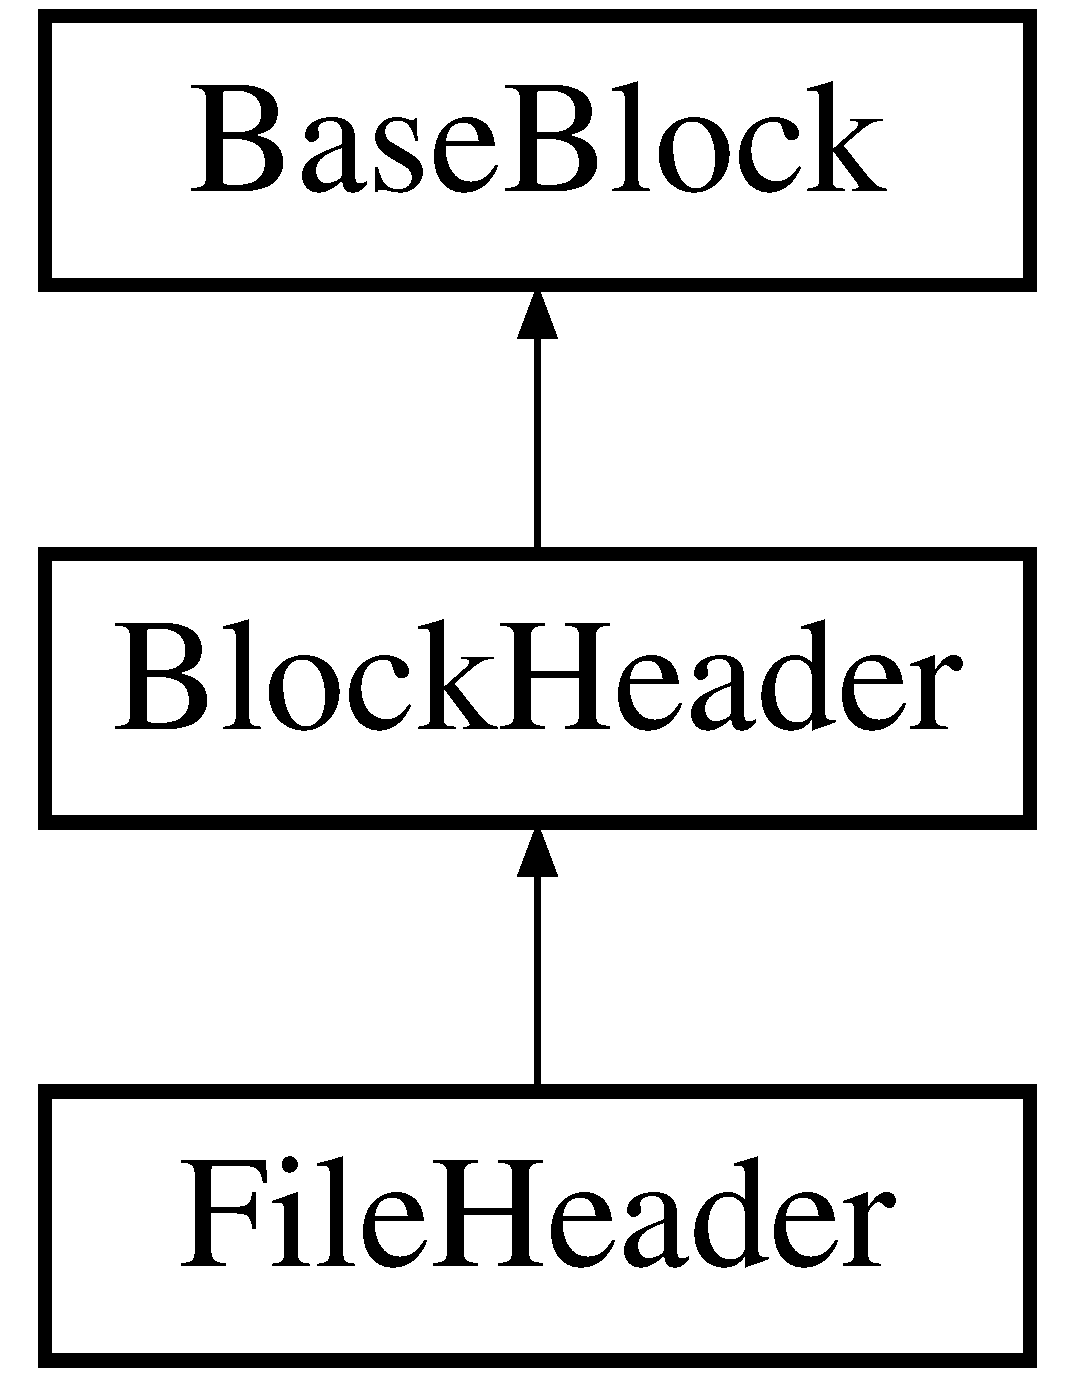
\includegraphics[height=3.000000cm]{struct_file_header}
\end{center}
\end{figure}
\subsection*{Public Member Functions}
\begin{DoxyCompactItemize}
\item 
\hypertarget{struct_file_header_a07a6fb68bc0122a2d062cbd510ee3a8c}{void {\bfseries Clear} (size\-\_\-t Sub\-Data\-Size)}\label{struct_file_header_a07a6fb68bc0122a2d062cbd510ee3a8c}

\item 
\hypertarget{struct_file_header_ad889a34882f468cf57a472b4d7357916}{bool {\bfseries Cmp\-Name} (const char $\ast$Name)}\label{struct_file_header_ad889a34882f468cf57a472b4d7357916}

\item 
\hypertarget{struct_file_header_a30611ab983d5982b3720f0f297f5205c}{\hyperlink{struct_file_header}{File\-Header} \& {\bfseries operator=} (\hyperlink{struct_file_header}{File\-Header} \&hd)}\label{struct_file_header_a30611ab983d5982b3720f0f297f5205c}

\end{DoxyCompactItemize}
\subsection*{Public Attributes}
\begin{DoxyCompactItemize}
\item 
\hypertarget{struct_file_header_a8522e15dd6bb8e331dfd22e1f72ed9a3}{uint {\bfseries Unp\-Size}}\label{struct_file_header_a8522e15dd6bb8e331dfd22e1f72ed9a3}

\item 
\hypertarget{struct_file_header_acfba02173c7ab6813720030dca602ce4}{byte {\bfseries Host\-O\-S}}\label{struct_file_header_acfba02173c7ab6813720030dca602ce4}

\item 
\hypertarget{struct_file_header_a33aa89dc8a1406752c28ddb6e25167e2}{uint {\bfseries File\-C\-R\-C}}\label{struct_file_header_a33aa89dc8a1406752c28ddb6e25167e2}

\item 
\hypertarget{struct_file_header_af50742777c9c6a0dfd374015736ced8b}{uint {\bfseries File\-Time}}\label{struct_file_header_af50742777c9c6a0dfd374015736ced8b}

\item 
\hypertarget{struct_file_header_a93cc842061209a5621e8cc995075178e}{byte {\bfseries Unp\-Ver}}\label{struct_file_header_a93cc842061209a5621e8cc995075178e}

\item 
\hypertarget{struct_file_header_a72a2b2af097d0268ef9e18e8e18e3ba7}{byte {\bfseries Method}}\label{struct_file_header_a72a2b2af097d0268ef9e18e8e18e3ba7}

\item 
\hypertarget{struct_file_header_a3b93d683023108786e5f41d7c5f0b72e}{ushort {\bfseries Name\-Size}}\label{struct_file_header_a3b93d683023108786e5f41d7c5f0b72e}

\item 
\hypertarget{struct_file_header_acfca1a9aabc5ebbda5e1c03c20a650f1}{\begin{tabbing}
xx\=xx\=xx\=xx\=xx\=xx\=xx\=xx\=xx\=\kill
union \{\\
\>uint {\bfseries FileAttr}\\
\>uint {\bfseries SubFlags}\\
\}; }\label{struct_file_header_acfca1a9aabc5ebbda5e1c03c20a650f1}
\\

\end{tabbing}\item 
\hypertarget{struct_file_header_ac84d8341c1635e0e969232b83533a4a0}{uint {\bfseries High\-Pack\-Size}}\label{struct_file_header_ac84d8341c1635e0e969232b83533a4a0}

\item 
\hypertarget{struct_file_header_abc7511a308607e4ca0a43952ce034fea}{uint {\bfseries High\-Unp\-Size}}\label{struct_file_header_abc7511a308607e4ca0a43952ce034fea}

\item 
\hypertarget{struct_file_header_a55f1028c28e452debab78582df25d1cd}{char {\bfseries File\-Name} \mbox{[}N\-M\mbox{]}}\label{struct_file_header_a55f1028c28e452debab78582df25d1cd}

\item 
\hypertarget{struct_file_header_a76786fbb1426d57adbf9642ad69a70ca}{wchar {\bfseries File\-Name\-W} \mbox{[}N\-M\mbox{]}}\label{struct_file_header_a76786fbb1426d57adbf9642ad69a70ca}

\item 
\hypertarget{struct_file_header_ab233d66624d5d2599afa67e7da75f648}{\hyperlink{class_array}{Array}$<$ byte $>$ {\bfseries Sub\-Data}}\label{struct_file_header_ab233d66624d5d2599afa67e7da75f648}

\item 
\hypertarget{struct_file_header_a9e543079bb0dbadb4b82c0ee85a4f5ba}{byte {\bfseries Salt} \mbox{[}S\-A\-L\-T\-\_\-\-S\-I\-Z\-E\mbox{]}}\label{struct_file_header_a9e543079bb0dbadb4b82c0ee85a4f5ba}

\item 
\hypertarget{struct_file_header_ac3832136560d3f982141f815984f637c}{\hyperlink{class_rar_time}{Rar\-Time} {\bfseries mtime}}\label{struct_file_header_ac3832136560d3f982141f815984f637c}

\item 
\hypertarget{struct_file_header_a4a3e06349dce2d56db21c7625e54b351}{\hyperlink{class_rar_time}{Rar\-Time} {\bfseries ctime}}\label{struct_file_header_a4a3e06349dce2d56db21c7625e54b351}

\item 
\hypertarget{struct_file_header_a007f826e5e2500d116163fdd5053858d}{\hyperlink{class_rar_time}{Rar\-Time} {\bfseries atime}}\label{struct_file_header_a007f826e5e2500d116163fdd5053858d}

\item 
\hypertarget{struct_file_header_ad100aeacb58dea2c1704fdee6f15bf5e}{\hyperlink{class_rar_time}{Rar\-Time} {\bfseries arctime}}\label{struct_file_header_ad100aeacb58dea2c1704fdee6f15bf5e}

\item 
\hypertarget{struct_file_header_a8e9137ea03d6351428f869df8be8d5f7}{int64 {\bfseries Full\-Pack\-Size}}\label{struct_file_header_a8e9137ea03d6351428f869df8be8d5f7}

\item 
\hypertarget{struct_file_header_a61d5b82cef4c18789734ea048206c064}{int64 {\bfseries Full\-Unp\-Size}}\label{struct_file_header_a61d5b82cef4c18789734ea048206c064}

\end{DoxyCompactItemize}


The documentation for this struct was generated from the following file\-:\begin{DoxyCompactItemize}
\item 
/\-Users/salazbr1/\-Documents/\-N\-P\-S/final\-\_\-unrarbulk\-\_\-extractor\-\_\-07-\/26-\/12/code/headers.\-hpp\end{DoxyCompactItemize}

\hypertarget{struct_file_stat}{\section{File\-Stat Struct Reference}
\label{struct_file_stat}\index{File\-Stat@{File\-Stat}}
}
\subsection*{Public Attributes}
\begin{DoxyCompactItemize}
\item 
\hypertarget{struct_file_stat_a4208c20f7cb8f4de40f969d868e23aa7}{uint {\bfseries File\-Attr}}\label{struct_file_stat_a4208c20f7cb8f4de40f969d868e23aa7}

\item 
\hypertarget{struct_file_stat_a44c9b84266cbafb72638cc917d402118}{uint {\bfseries File\-Time}}\label{struct_file_stat_a44c9b84266cbafb72638cc917d402118}

\item 
\hypertarget{struct_file_stat_a7dc9075fd5653be11684da2100df8730}{int64 {\bfseries File\-Size}}\label{struct_file_stat_a7dc9075fd5653be11684da2100df8730}

\item 
\hypertarget{struct_file_stat_ae7133c1062c235c174a801d896ec1cd1}{bool {\bfseries Is\-Dir}}\label{struct_file_stat_ae7133c1062c235c174a801d896ec1cd1}

\end{DoxyCompactItemize}


The documentation for this struct was generated from the following file\-:\begin{DoxyCompactItemize}
\item 
/\-Users/salazbr1/\-Documents/\-N\-P\-S/final\-\_\-unrarbulk\-\_\-extractor\-\_\-07-\/26-\/12/code/file.\-hpp\end{DoxyCompactItemize}

\hypertarget{struct_filter_mode}{\section{Filter\-Mode Struct Reference}
\label{struct_filter_mode}\index{Filter\-Mode@{Filter\-Mode}}
}
\subsection*{Public Attributes}
\begin{DoxyCompactItemize}
\item 
\hypertarget{struct_filter_mode_a8d19a744ad89d5f5d381e72066b75336}{Filter\-State {\bfseries State}}\label{struct_filter_mode_a8d19a744ad89d5f5d381e72066b75336}

\item 
\hypertarget{struct_filter_mode_a5e78aea0f97f3a49140bcc9ac94a4e84}{int {\bfseries Param1}}\label{struct_filter_mode_a5e78aea0f97f3a49140bcc9ac94a4e84}

\item 
\hypertarget{struct_filter_mode_ae642d181f77c007488a0e191d6e90f01}{int {\bfseries Param2}}\label{struct_filter_mode_ae642d181f77c007488a0e191d6e90f01}

\end{DoxyCompactItemize}


The documentation for this struct was generated from the following file\-:\begin{DoxyCompactItemize}
\item 
/\-Users/salazbr1/\-Documents/\-N\-P\-S/final\-\_\-unrarbulk\-\_\-extractor\-\_\-07-\/26-\/12/code/options.\-hpp\end{DoxyCompactItemize}

\hypertarget{struct_find_data}{\section{Find\-Data Struct Reference}
\label{struct_find_data}\index{Find\-Data@{Find\-Data}}
}
\subsection*{Public Attributes}
\begin{DoxyCompactItemize}
\item 
\hypertarget{struct_find_data_a20a349722b3f4c321a41c899b98ff92f}{char {\bfseries Name} \mbox{[}N\-M\mbox{]}}\label{struct_find_data_a20a349722b3f4c321a41c899b98ff92f}

\item 
\hypertarget{struct_find_data_a4d8b96033d8330b18fcb59929d81ef0a}{wchar {\bfseries Name\-W} \mbox{[}N\-M\mbox{]}}\label{struct_find_data_a4d8b96033d8330b18fcb59929d81ef0a}

\item 
\hypertarget{struct_find_data_a30f5982c4998f7d5dea652c4d3b29c39}{int64 {\bfseries Size}}\label{struct_find_data_a30f5982c4998f7d5dea652c4d3b29c39}

\item 
\hypertarget{struct_find_data_a8cf6201242e2bdb3743a968e9e221e1c}{uint {\bfseries File\-Attr}}\label{struct_find_data_a8cf6201242e2bdb3743a968e9e221e1c}

\item 
\hypertarget{struct_find_data_a592644ce87bdeba34a42b166f6e56cb3}{uint {\bfseries File\-Time}}\label{struct_find_data_a592644ce87bdeba34a42b166f6e56cb3}

\item 
\hypertarget{struct_find_data_af294fda4d711e5808fbfb87d3af95462}{bool {\bfseries Is\-Dir}}\label{struct_find_data_af294fda4d711e5808fbfb87d3af95462}

\item 
\hypertarget{struct_find_data_a0d6c787fcfe10839a7efb8a62425a6c2}{\hyperlink{class_rar_time}{Rar\-Time} {\bfseries mtime}}\label{struct_find_data_a0d6c787fcfe10839a7efb8a62425a6c2}

\item 
\hypertarget{struct_find_data_aea792dfa4b64278dc42c9a0a1a6b409b}{\hyperlink{class_rar_time}{Rar\-Time} {\bfseries ctime}}\label{struct_find_data_aea792dfa4b64278dc42c9a0a1a6b409b}

\item 
\hypertarget{struct_find_data_a052bd174bb0702bf987cc24916802b51}{\hyperlink{class_rar_time}{Rar\-Time} {\bfseries atime}}\label{struct_find_data_a052bd174bb0702bf987cc24916802b51}

\item 
\hypertarget{struct_find_data_a75c29a8fe2f236f688c98b877c67bac2}{uint {\bfseries Flags}}\label{struct_find_data_a75c29a8fe2f236f688c98b877c67bac2}

\item 
\hypertarget{struct_find_data_ab891d3e368f9c03b16a685c13279ad96}{bool {\bfseries Error}}\label{struct_find_data_ab891d3e368f9c03b16a685c13279ad96}

\end{DoxyCompactItemize}


The documentation for this struct was generated from the following file\-:\begin{DoxyCompactItemize}
\item 
/\-Users/salazbr1/\-Documents/\-N\-P\-S/final\-\_\-unrarbulk\-\_\-extractor\-\_\-07-\/26-\/12/code/find.\-hpp\end{DoxyCompactItemize}

\hypertarget{class_find_file}{\section{Find\-File Class Reference}
\label{class_find_file}\index{Find\-File@{Find\-File}}
}
\subsection*{Public Member Functions}
\begin{DoxyCompactItemize}
\item 
\hypertarget{class_find_file_ae4e73fe2efdf1bd7d1d788a050ab473e}{void {\bfseries Set\-Mask} (const char $\ast$Find\-Mask)}\label{class_find_file_ae4e73fe2efdf1bd7d1d788a050ab473e}

\item 
\hypertarget{class_find_file_a60fd077790df2c0b3f299fd64bd7b174}{void {\bfseries Set\-Mask\-W} (const wchar $\ast$Find\-Mask\-W)}\label{class_find_file_a60fd077790df2c0b3f299fd64bd7b174}

\item 
\hypertarget{class_find_file_ad18c9bbc6c1e15950d3fdd2eece060cc}{bool {\bfseries Next} (\hyperlink{struct_find_data}{Find\-Data} $\ast$fd, bool Get\-Sym\-Link=false)}\label{class_find_file_ad18c9bbc6c1e15950d3fdd2eece060cc}

\end{DoxyCompactItemize}
\subsection*{Static Public Member Functions}
\begin{DoxyCompactItemize}
\item 
\hypertarget{class_find_file_a1174d97544c272d4ce5ba92dc1dc5112}{static bool {\bfseries Fast\-Find} (const char $\ast$Find\-Mask, const wchar $\ast$Find\-Mask\-W, \hyperlink{struct_find_data}{Find\-Data} $\ast$fd, bool Get\-Sym\-Link=false)}\label{class_find_file_a1174d97544c272d4ce5ba92dc1dc5112}

\end{DoxyCompactItemize}


The documentation for this class was generated from the following files\-:\begin{DoxyCompactItemize}
\item 
/\-Users/salazbr1/\-Documents/\-N\-P\-S/final\-\_\-unrarbulk\-\_\-extractor\-\_\-07-\/26-\/12/code/find.\-hpp\item 
/\-Users/salazbr1/\-Documents/\-N\-P\-S/final\-\_\-unrarbulk\-\_\-extractor\-\_\-07-\/26-\/12/code/find.\-cpp\end{DoxyCompactItemize}

\hypertarget{struct_freq_data}{\section{Freq\-Data Struct Reference}
\label{struct_freq_data}\index{Freq\-Data@{Freq\-Data}}
}
\subsection*{Public Attributes}
\begin{DoxyCompactItemize}
\item 
\hypertarget{struct_freq_data_a191cac4679a18afa6ece469aee3846a7}{ushort {\bfseries Summ\-Freq}}\label{struct_freq_data_a191cac4679a18afa6ece469aee3846a7}

\item 
\hypertarget{struct_freq_data_a114ed6d41a3b8df8c39ba3d1917ee76b}{\hyperlink{struct_s_t_a_t_e}{S\-T\-A\-T\-E} \-\_\-\-P\-A\-C\-K\-\_\-\-A\-T\-T\-R $\ast$ {\bfseries Stats}}\label{struct_freq_data_a114ed6d41a3b8df8c39ba3d1917ee76b}

\end{DoxyCompactItemize}


The documentation for this struct was generated from the following file\-:\begin{DoxyCompactItemize}
\item 
/\-Users/salazbr1/\-Documents/\-N\-P\-S/final\-\_\-unrarbulk\-\_\-extractor\-\_\-07-\/26-\/12/code/model.\-hpp\end{DoxyCompactItemize}

\hypertarget{structhash__context}{\section{hash\-\_\-context Struct Reference}
\label{structhash__context}\index{hash\-\_\-context@{hash\-\_\-context}}
}
\subsection*{Public Attributes}
\begin{DoxyCompactItemize}
\item 
\hypertarget{structhash__context_ae741feeba04e89a487b7180198b98b27}{uint32 {\bfseries state} \mbox{[}5\mbox{]}}\label{structhash__context_ae741feeba04e89a487b7180198b98b27}

\item 
\hypertarget{structhash__context_ae0c487dd20545403d7ede0120b2a0891}{uint32 {\bfseries count} \mbox{[}2\mbox{]}}\label{structhash__context_ae0c487dd20545403d7ede0120b2a0891}

\item 
\hypertarget{structhash__context_a7ff05817f73a181740899409a638fd90}{unsigned char {\bfseries buffer} \mbox{[}64\mbox{]}}\label{structhash__context_a7ff05817f73a181740899409a638fd90}

\item 
\hypertarget{structhash__context_a9df344022f9410bdd8311791396735f6}{unsigned char {\bfseries workspace} \mbox{[}64\mbox{]}}\label{structhash__context_a9df344022f9410bdd8311791396735f6}

\end{DoxyCompactItemize}


The documentation for this struct was generated from the following file\-:\begin{DoxyCompactItemize}
\item 
/\-Users/salazbr1/\-Documents/\-N\-P\-S/final\-\_\-unrarbulk\-\_\-extractor\-\_\-07-\/26-\/12/code/sha1.\-hpp\end{DoxyCompactItemize}

\hypertarget{struct_mac_f_info_header}{\section{Mac\-F\-Info\-Header Struct Reference}
\label{struct_mac_f_info_header}\index{Mac\-F\-Info\-Header@{Mac\-F\-Info\-Header}}
}
Inheritance diagram for Mac\-F\-Info\-Header\-:\begin{figure}[H]
\begin{center}
\leavevmode
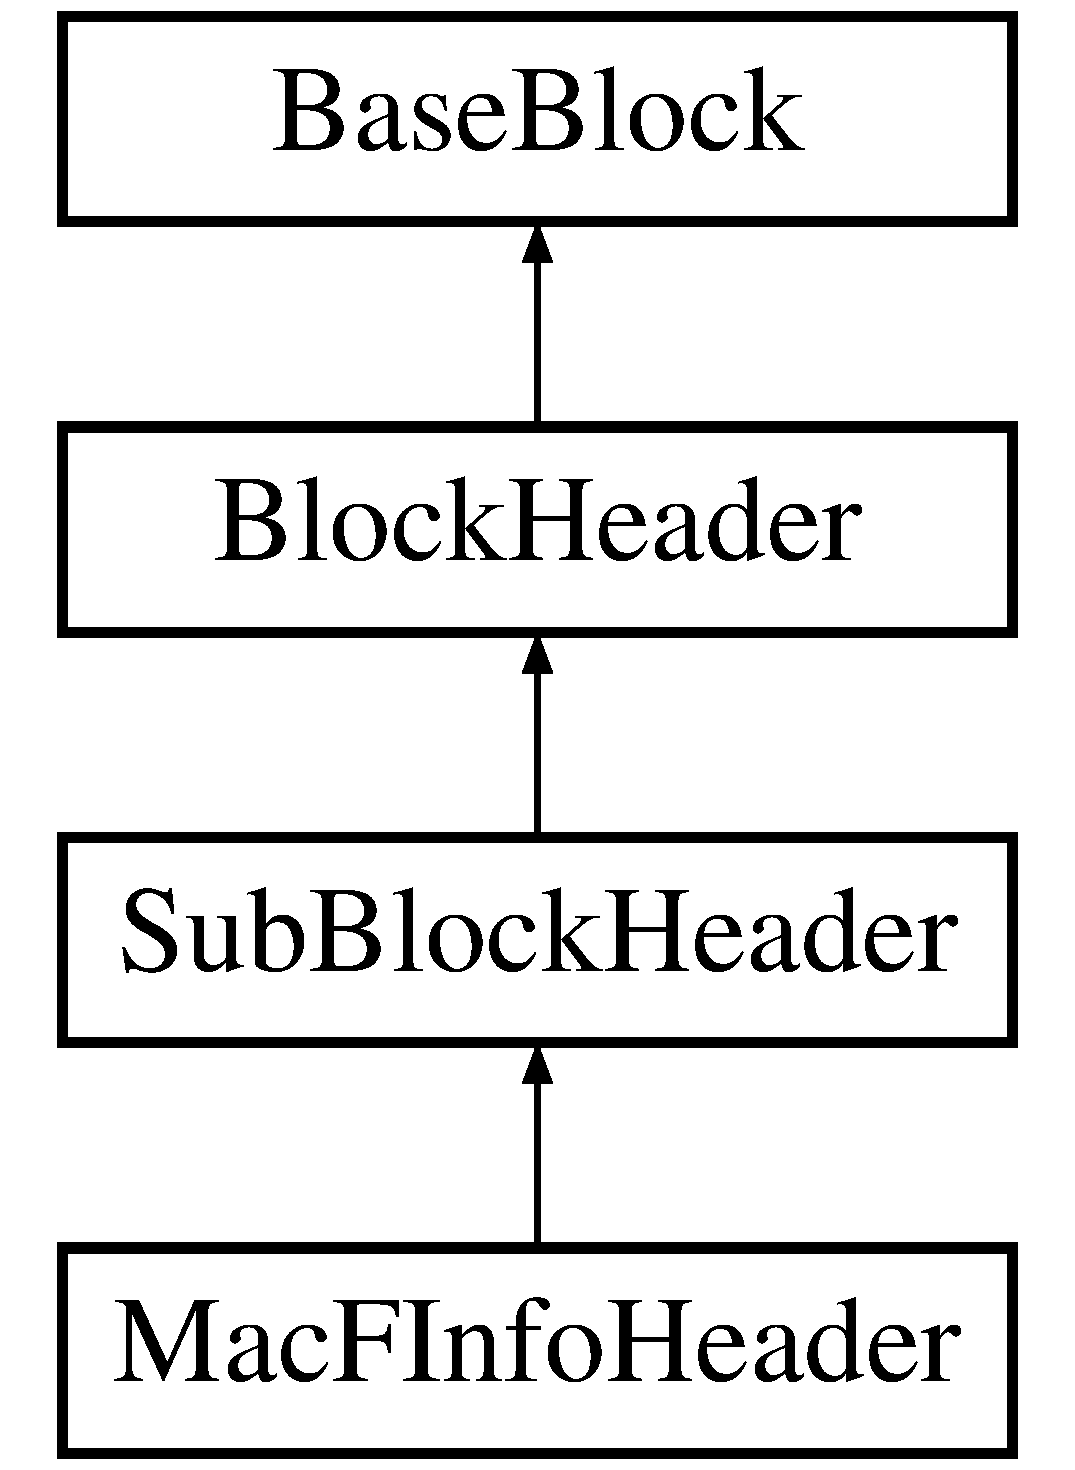
\includegraphics[height=4.000000cm]{struct_mac_f_info_header}
\end{center}
\end{figure}
\subsection*{Public Attributes}
\begin{DoxyCompactItemize}
\item 
\hypertarget{struct_mac_f_info_header_a92850562e6d62075301dfbb8342e8080}{uint {\bfseries file\-Type}}\label{struct_mac_f_info_header_a92850562e6d62075301dfbb8342e8080}

\item 
\hypertarget{struct_mac_f_info_header_abbfce87f4474e5700a5c02717e9201da}{uint {\bfseries file\-Creator}}\label{struct_mac_f_info_header_abbfce87f4474e5700a5c02717e9201da}

\end{DoxyCompactItemize}


The documentation for this struct was generated from the following file\-:\begin{DoxyCompactItemize}
\item 
/\-Users/salazbr1/\-Documents/\-N\-P\-S/final\-\_\-unrarbulk\-\_\-extractor\-\_\-07-\/26-\/12/code/headers.\-hpp\end{DoxyCompactItemize}

\hypertarget{struct_main_header}{\section{Main\-Header Struct Reference}
\label{struct_main_header}\index{Main\-Header@{Main\-Header}}
}
Inheritance diagram for Main\-Header\-:\begin{figure}[H]
\begin{center}
\leavevmode
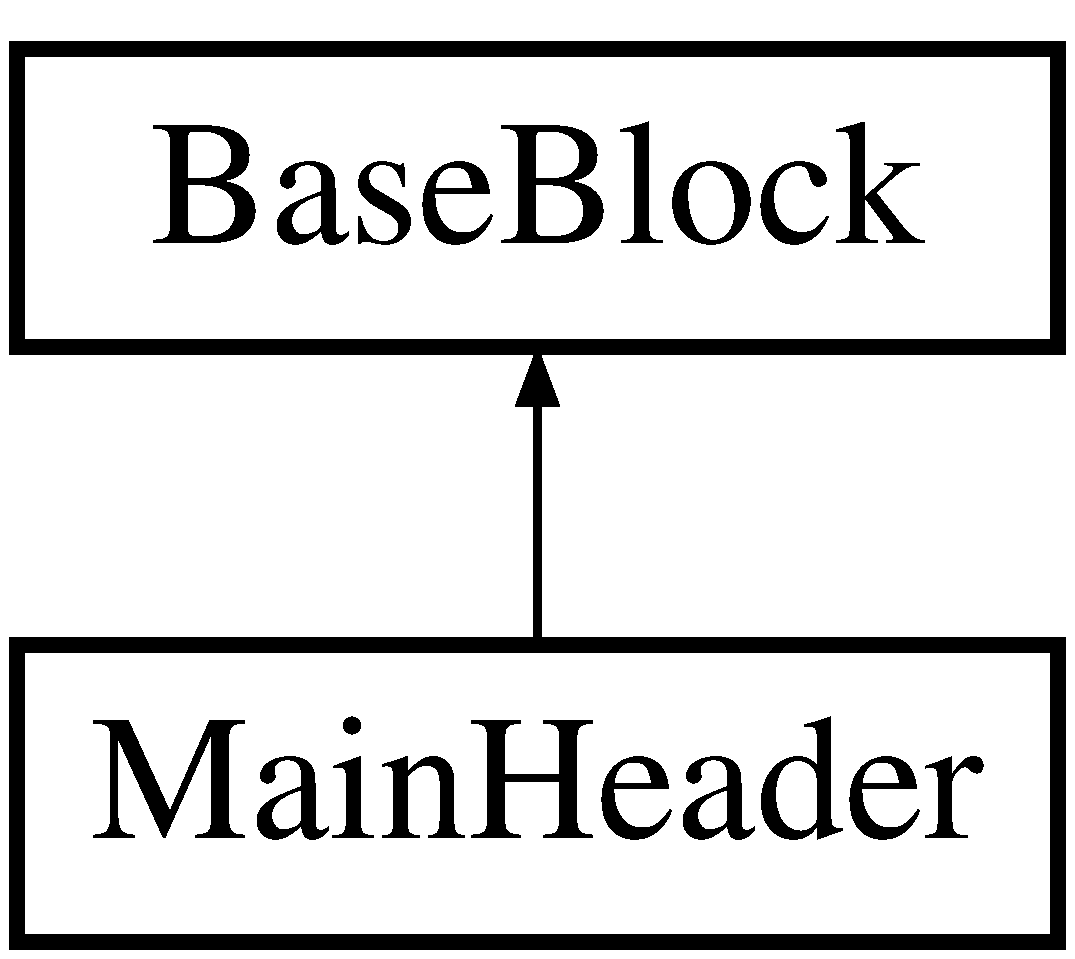
\includegraphics[height=2.000000cm]{struct_main_header}
\end{center}
\end{figure}
\subsection*{Public Attributes}
\begin{DoxyCompactItemize}
\item 
\hypertarget{struct_main_header_a7bde589c13d97233aaece964d12cf7af}{ushort {\bfseries High\-Pos\-A\-V}}\label{struct_main_header_a7bde589c13d97233aaece964d12cf7af}

\item 
\hypertarget{struct_main_header_a97917545b4b775253b60b8d7f83e112e}{uint {\bfseries Pos\-A\-V}}\label{struct_main_header_a97917545b4b775253b60b8d7f83e112e}

\item 
\hypertarget{struct_main_header_a0a500814f7e4758d8c0bc14108b05aa0}{byte {\bfseries Encrypt\-Ver}}\label{struct_main_header_a0a500814f7e4758d8c0bc14108b05aa0}

\end{DoxyCompactItemize}
\subsection*{Additional Inherited Members}


The documentation for this struct was generated from the following file\-:\begin{DoxyCompactItemize}
\item 
/\-Users/salazbr1/\-Documents/\-N\-P\-S/final\-\_\-unrarbulk\-\_\-extractor\-\_\-07-\/26-\/12/code/headers.\-hpp\end{DoxyCompactItemize}

\hypertarget{struct_mark_header}{\section{Mark\-Header Struct Reference}
\label{struct_mark_header}\index{Mark\-Header@{Mark\-Header}}
}
\subsection*{Public Attributes}
\begin{DoxyCompactItemize}
\item 
\hypertarget{struct_mark_header_a879657ef67ef42dbfa01346f7afdab01}{byte {\bfseries Mark} \mbox{[}7\mbox{]}}\label{struct_mark_header_a879657ef67ef42dbfa01346f7afdab01}

\end{DoxyCompactItemize}


The documentation for this struct was generated from the following file\-:\begin{DoxyCompactItemize}
\item 
/\-Users/salazbr1/\-Documents/\-N\-P\-S/final\-\_\-unrarbulk\-\_\-extractor\-\_\-07-\/26-\/12/code/headers.\-hpp\end{DoxyCompactItemize}

\hypertarget{class_model_p_p_m}{\section{Model\-P\-P\-M Class Reference}
\label{class_model_p_p_m}\index{Model\-P\-P\-M@{Model\-P\-P\-M}}
}
\subsection*{Public Member Functions}
\begin{DoxyCompactItemize}
\item 
\hypertarget{class_model_p_p_m_a73f7b37ca222c1705b21c77bc087517e}{void {\bfseries Clean\-Up} ()}\label{class_model_p_p_m_a73f7b37ca222c1705b21c77bc087517e}

\item 
\hypertarget{class_model_p_p_m_a7c1dee7a9683ad952691f97b71dda662}{bool {\bfseries Decode\-Init} (\hyperlink{class_unpack}{Unpack} $\ast$Unpack\-Read, int \&Esc\-Char)}\label{class_model_p_p_m_a7c1dee7a9683ad952691f97b71dda662}

\item 
\hypertarget{class_model_p_p_m_a87f01605ccdedca3d27b218b2a0b9e56}{int {\bfseries Decode\-Char} ()}\label{class_model_p_p_m_a87f01605ccdedca3d27b218b2a0b9e56}

\end{DoxyCompactItemize}
\subsection*{Friends}
\begin{DoxyCompactItemize}
\item 
\hypertarget{class_model_p_p_m_a66489b21d67f04d21aa22be31740a628}{struct {\bfseries P\-P\-M\-\_\-\-C\-O\-N\-T\-E\-X\-T}}\label{class_model_p_p_m_a66489b21d67f04d21aa22be31740a628}

\end{DoxyCompactItemize}


The documentation for this class was generated from the following files\-:\begin{DoxyCompactItemize}
\item 
/\-Users/salazbr1/\-Documents/\-N\-P\-S/final\-\_\-unrarbulk\-\_\-extractor\-\_\-07-\/26-\/12/code/model.\-hpp\item 
/\-Users/salazbr1/\-Documents/\-N\-P\-S/final\-\_\-unrarbulk\-\_\-extractor\-\_\-07-\/26-\/12/code/model.\-cpp\end{DoxyCompactItemize}

\hypertarget{struct_old_file_header}{\section{Old\-File\-Header Struct Reference}
\label{struct_old_file_header}\index{Old\-File\-Header@{Old\-File\-Header}}
}
\subsection*{Public Attributes}
\begin{DoxyCompactItemize}
\item 
\hypertarget{struct_old_file_header_a7b1735ad8d5e23d7925d071e6dbf38db}{uint {\bfseries Pack\-Size}}\label{struct_old_file_header_a7b1735ad8d5e23d7925d071e6dbf38db}

\item 
\hypertarget{struct_old_file_header_af4970281150a01d1a805cf7417e0e197}{uint {\bfseries Unp\-Size}}\label{struct_old_file_header_af4970281150a01d1a805cf7417e0e197}

\item 
\hypertarget{struct_old_file_header_a53837ac16c3745705f8dd58c06b02a80}{ushort {\bfseries File\-C\-R\-C}}\label{struct_old_file_header_a53837ac16c3745705f8dd58c06b02a80}

\item 
\hypertarget{struct_old_file_header_a80e51a5f91d58c143bba8d1c1bf757aa}{ushort {\bfseries Head\-Size}}\label{struct_old_file_header_a80e51a5f91d58c143bba8d1c1bf757aa}

\item 
\hypertarget{struct_old_file_header_aa9bba2bc62e140533da8f99aac194e21}{uint {\bfseries File\-Time}}\label{struct_old_file_header_aa9bba2bc62e140533da8f99aac194e21}

\item 
\hypertarget{struct_old_file_header_a1418f4ae642623910e4f387e1847af91}{byte {\bfseries File\-Attr}}\label{struct_old_file_header_a1418f4ae642623910e4f387e1847af91}

\item 
\hypertarget{struct_old_file_header_a49213b0b149475b674539aaeaece088b}{byte {\bfseries Flags}}\label{struct_old_file_header_a49213b0b149475b674539aaeaece088b}

\item 
\hypertarget{struct_old_file_header_ae08e7e3407437e6539cf9602bc2a87c4}{byte {\bfseries Unp\-Ver}}\label{struct_old_file_header_ae08e7e3407437e6539cf9602bc2a87c4}

\item 
\hypertarget{struct_old_file_header_ac18d5ecb73221a0edd7e74f7867a289c}{byte {\bfseries Name\-Size}}\label{struct_old_file_header_ac18d5ecb73221a0edd7e74f7867a289c}

\item 
\hypertarget{struct_old_file_header_a5195793688cf9505956a295368e2f68d}{byte {\bfseries Method}}\label{struct_old_file_header_a5195793688cf9505956a295368e2f68d}

\end{DoxyCompactItemize}


The documentation for this struct was generated from the following file\-:\begin{DoxyCompactItemize}
\item 
/\-Users/salazbr1/\-Documents/\-N\-P\-S/final\-\_\-unrarbulk\-\_\-extractor\-\_\-07-\/26-\/12/code/headers.\-hpp\end{DoxyCompactItemize}

\hypertarget{struct_old_main_header}{\section{Old\-Main\-Header Struct Reference}
\label{struct_old_main_header}\index{Old\-Main\-Header@{Old\-Main\-Header}}
}
\subsection*{Public Attributes}
\begin{DoxyCompactItemize}
\item 
\hypertarget{struct_old_main_header_a46c68916cfde9a3a4edb0f5cfb005ed3}{byte {\bfseries Mark} \mbox{[}4\mbox{]}}\label{struct_old_main_header_a46c68916cfde9a3a4edb0f5cfb005ed3}

\item 
\hypertarget{struct_old_main_header_a292e53b3eaf681ece34767b683515ab9}{ushort {\bfseries Head\-Size}}\label{struct_old_main_header_a292e53b3eaf681ece34767b683515ab9}

\item 
\hypertarget{struct_old_main_header_a24f364ad492dc28c43e58e4d55d8978c}{byte {\bfseries Flags}}\label{struct_old_main_header_a24f364ad492dc28c43e58e4d55d8978c}

\end{DoxyCompactItemize}


The documentation for this struct was generated from the following file\-:\begin{DoxyCompactItemize}
\item 
/\-Users/salazbr1/\-Documents/\-N\-P\-S/final\-\_\-unrarbulk\-\_\-extractor\-\_\-07-\/26-\/12/code/headers.\-hpp\end{DoxyCompactItemize}

\hypertarget{struct_p_p_m___c_o_n_t_e_x_t}{\section{P\-P\-M\-\_\-\-C\-O\-N\-T\-E\-X\-T Struct Reference}
\label{struct_p_p_m___c_o_n_t_e_x_t}\index{P\-P\-M\-\_\-\-C\-O\-N\-T\-E\-X\-T@{P\-P\-M\-\_\-\-C\-O\-N\-T\-E\-X\-T}}
}
\subsection*{Public Member Functions}
\begin{DoxyCompactItemize}
\item 
\hypertarget{struct_p_p_m___c_o_n_t_e_x_t_aca54b416b67385bfc184af3324076872}{void {\bfseries encode\-Bin\-Symbol} (\hyperlink{class_model_p_p_m}{Model\-P\-P\-M} $\ast$Model, int symbol)}\label{struct_p_p_m___c_o_n_t_e_x_t_aca54b416b67385bfc184af3324076872}

\item 
\hypertarget{struct_p_p_m___c_o_n_t_e_x_t_a71656afab0ae5486d00709235fdacfc5}{void {\bfseries encode\-Symbol1} (\hyperlink{class_model_p_p_m}{Model\-P\-P\-M} $\ast$Model, int symbol)}\label{struct_p_p_m___c_o_n_t_e_x_t_a71656afab0ae5486d00709235fdacfc5}

\item 
\hypertarget{struct_p_p_m___c_o_n_t_e_x_t_af10c3c49128d844dd3348741f6aec81f}{void {\bfseries encode\-Symbol2} (\hyperlink{class_model_p_p_m}{Model\-P\-P\-M} $\ast$Model, int symbol)}\label{struct_p_p_m___c_o_n_t_e_x_t_af10c3c49128d844dd3348741f6aec81f}

\item 
\hypertarget{struct_p_p_m___c_o_n_t_e_x_t_a1f2d13441e65a192e48c5b140b3d3440}{void {\bfseries decode\-Bin\-Symbol} (\hyperlink{class_model_p_p_m}{Model\-P\-P\-M} $\ast$Model)}\label{struct_p_p_m___c_o_n_t_e_x_t_a1f2d13441e65a192e48c5b140b3d3440}

\item 
\hypertarget{struct_p_p_m___c_o_n_t_e_x_t_af2e9116c0b979e06eaf058f0254ea2ba}{bool {\bfseries decode\-Symbol1} (\hyperlink{class_model_p_p_m}{Model\-P\-P\-M} $\ast$Model)}\label{struct_p_p_m___c_o_n_t_e_x_t_af2e9116c0b979e06eaf058f0254ea2ba}

\item 
\hypertarget{struct_p_p_m___c_o_n_t_e_x_t_aaeb6637b300edf35c2302db58f5a7eea}{bool {\bfseries decode\-Symbol2} (\hyperlink{class_model_p_p_m}{Model\-P\-P\-M} $\ast$Model)}\label{struct_p_p_m___c_o_n_t_e_x_t_aaeb6637b300edf35c2302db58f5a7eea}

\item 
\hypertarget{struct_p_p_m___c_o_n_t_e_x_t_a434b490c618ed763873c87373bb13439}{void {\bfseries update1} (\hyperlink{class_model_p_p_m}{Model\-P\-P\-M} $\ast$Model, \hyperlink{struct_s_t_a_t_e}{S\-T\-A\-T\-E} $\ast$p)}\label{struct_p_p_m___c_o_n_t_e_x_t_a434b490c618ed763873c87373bb13439}

\item 
\hypertarget{struct_p_p_m___c_o_n_t_e_x_t_ad75dbbf75bc362af1bd5279760eb4402}{void {\bfseries update2} (\hyperlink{class_model_p_p_m}{Model\-P\-P\-M} $\ast$Model, \hyperlink{struct_s_t_a_t_e}{S\-T\-A\-T\-E} $\ast$p)}\label{struct_p_p_m___c_o_n_t_e_x_t_ad75dbbf75bc362af1bd5279760eb4402}

\item 
\hypertarget{struct_p_p_m___c_o_n_t_e_x_t_a6602e3e590060f0b0d318a6f62049094}{void {\bfseries rescale} (\hyperlink{class_model_p_p_m}{Model\-P\-P\-M} $\ast$Model)}\label{struct_p_p_m___c_o_n_t_e_x_t_a6602e3e590060f0b0d318a6f62049094}

\item 
\hypertarget{struct_p_p_m___c_o_n_t_e_x_t_a00270a520aed5f4d6ce2844bbcbf014a}{\hyperlink{struct_p_p_m___c_o_n_t_e_x_t}{P\-P\-M\-\_\-\-C\-O\-N\-T\-E\-X\-T} $\ast$ {\bfseries create\-Child} (\hyperlink{class_model_p_p_m}{Model\-P\-P\-M} $\ast$Model, \hyperlink{struct_s_t_a_t_e}{S\-T\-A\-T\-E} $\ast$p\-Stats, \hyperlink{struct_s_t_a_t_e}{S\-T\-A\-T\-E} \&First\-State)}\label{struct_p_p_m___c_o_n_t_e_x_t_a00270a520aed5f4d6ce2844bbcbf014a}

\item 
\hypertarget{struct_p_p_m___c_o_n_t_e_x_t_ae9f3acb5c7ef9b8e35f690b10379e554}{\hyperlink{struct_s_e_e2___c_o_n_t_e_x_t}{S\-E\-E2\-\_\-\-C\-O\-N\-T\-E\-X\-T} $\ast$ {\bfseries make\-Esc\-Freq2} (\hyperlink{class_model_p_p_m}{Model\-P\-P\-M} $\ast$Model, int Diff)}\label{struct_p_p_m___c_o_n_t_e_x_t_ae9f3acb5c7ef9b8e35f690b10379e554}

\end{DoxyCompactItemize}
\subsection*{Public Attributes}
\begin{DoxyCompactItemize}
\item 
\hypertarget{struct_p_p_m___c_o_n_t_e_x_t_af4615f7c4a6b787970ee62e4f736ca04}{ushort {\bfseries Num\-Stats}}\label{struct_p_p_m___c_o_n_t_e_x_t_af4615f7c4a6b787970ee62e4f736ca04}

\item 
\hypertarget{struct_p_p_m___c_o_n_t_e_x_t_a536ca27885309a53d349ffa9e2dc1a91}{\begin{tabbing}
xx\=xx\=xx\=xx\=xx\=xx\=xx\=xx\=xx\=\kill
union \{\\
\>\hyperlink{struct_freq_data}{FreqData} {\bfseries U}\\
\>\hyperlink{struct_s_t_a_t_e}{STATE} {\bfseries OneState}\\
\}; }\label{struct_p_p_m___c_o_n_t_e_x_t_a536ca27885309a53d349ffa9e2dc1a91}
\\

\end{tabbing}\item 
\hypertarget{struct_p_p_m___c_o_n_t_e_x_t_ae5701bbb65f7d55de50811bdf21e8be4}{\hyperlink{struct_p_p_m___c_o_n_t_e_x_t}{P\-P\-M\-\_\-\-C\-O\-N\-T\-E\-X\-T} $\ast$ {\bfseries Suffix}}\label{struct_p_p_m___c_o_n_t_e_x_t_ae5701bbb65f7d55de50811bdf21e8be4}

\end{DoxyCompactItemize}


The documentation for this struct was generated from the following files\-:\begin{DoxyCompactItemize}
\item 
/\-Users/salazbr1/\-Documents/\-N\-P\-S/final\-\_\-unrarbulk\-\_\-extractor\-\_\-07-\/26-\/12/code/model.\-hpp\item 
/\-Users/salazbr1/\-Documents/\-N\-P\-S/final\-\_\-unrarbulk\-\_\-extractor\-\_\-07-\/26-\/12/code/model.\-cpp\end{DoxyCompactItemize}

\hypertarget{struct_protect_header}{\section{Protect\-Header Struct Reference}
\label{struct_protect_header}\index{Protect\-Header@{Protect\-Header}}
}
Inheritance diagram for Protect\-Header\-:\begin{figure}[H]
\begin{center}
\leavevmode
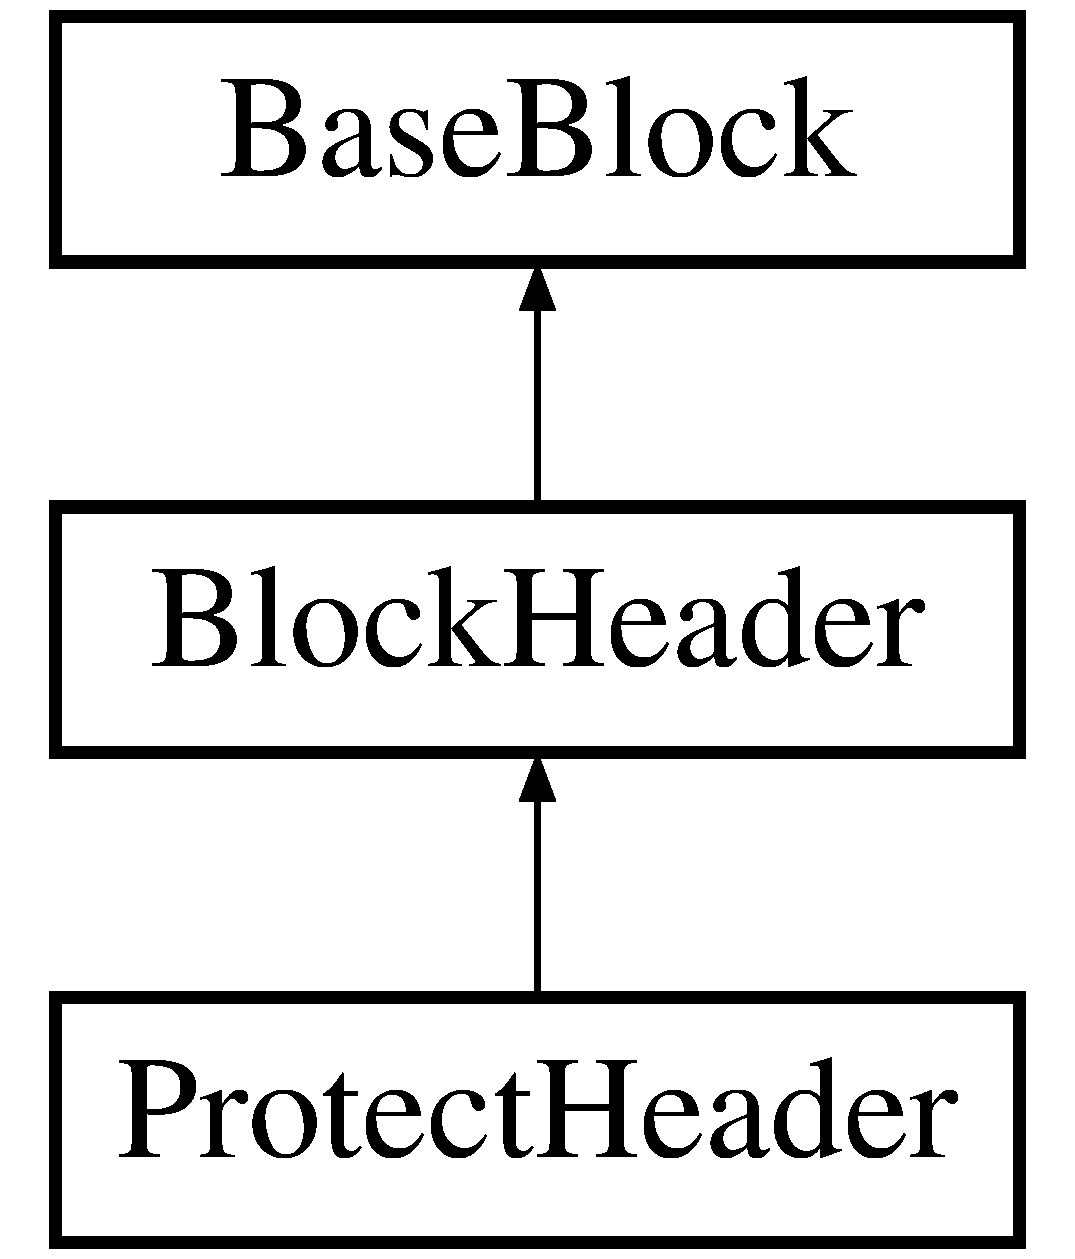
\includegraphics[height=3.000000cm]{struct_protect_header}
\end{center}
\end{figure}
\subsection*{Public Attributes}
\begin{DoxyCompactItemize}
\item 
\hypertarget{struct_protect_header_a6cd775ee9658f19a25765d225955783b}{byte {\bfseries Version}}\label{struct_protect_header_a6cd775ee9658f19a25765d225955783b}

\item 
\hypertarget{struct_protect_header_a88eb56ba56a776a62b1d081e46ebb1eb}{ushort {\bfseries Rec\-Sectors}}\label{struct_protect_header_a88eb56ba56a776a62b1d081e46ebb1eb}

\item 
\hypertarget{struct_protect_header_a3cab4857a0abda2c5bcab0f92e69daca}{uint {\bfseries Total\-Blocks}}\label{struct_protect_header_a3cab4857a0abda2c5bcab0f92e69daca}

\item 
\hypertarget{struct_protect_header_ad9f86b9e6e52b1db7904cabd06beb6bb}{byte {\bfseries Mark} \mbox{[}8\mbox{]}}\label{struct_protect_header_ad9f86b9e6e52b1db7904cabd06beb6bb}

\end{DoxyCompactItemize}


The documentation for this struct was generated from the following file\-:\begin{DoxyCompactItemize}
\item 
/\-Users/salazbr1/\-Documents/\-N\-P\-S/final\-\_\-unrarbulk\-\_\-extractor\-\_\-07-\/26-\/12/code/headers.\-hpp\end{DoxyCompactItemize}

\hypertarget{class_range_coder}{\section{Range\-Coder Class Reference}
\label{class_range_coder}\index{Range\-Coder@{Range\-Coder}}
}
\subsection*{Classes}
\begin{DoxyCompactItemize}
\item 
struct \hyperlink{struct_range_coder_1_1_s_u_b_r_a_n_g_e}{S\-U\-B\-R\-A\-N\-G\-E}
\end{DoxyCompactItemize}
\subsection*{Public Member Functions}
\begin{DoxyCompactItemize}
\item 
\hypertarget{class_range_coder_acd9c3a3dbe80ffe3c7613a8a6a4387aa}{void {\bfseries Init\-Decoder} (\hyperlink{class_unpack}{Unpack} $\ast$Unpack\-Read)}\label{class_range_coder_acd9c3a3dbe80ffe3c7613a8a6a4387aa}

\item 
\hypertarget{class_range_coder_a134cd616672190977b018c4458f41122}{int {\bfseries Get\-Current\-Count} ()}\label{class_range_coder_a134cd616672190977b018c4458f41122}

\item 
\hypertarget{class_range_coder_aa9974b9aaf835e26b4527bc42085e6b5}{uint {\bfseries Get\-Current\-Shift\-Count} (uint S\-H\-I\-F\-T)}\label{class_range_coder_aa9974b9aaf835e26b4527bc42085e6b5}

\item 
\hypertarget{class_range_coder_a909c39b5c0c2c2409660f3b5446f1d3c}{void {\bfseries Decode} ()}\label{class_range_coder_a909c39b5c0c2c2409660f3b5446f1d3c}

\item 
\hypertarget{class_range_coder_a332571b493b532f5f3b91abee33c5e5e}{void {\bfseries Put\-Char} (unsigned int c)}\label{class_range_coder_a332571b493b532f5f3b91abee33c5e5e}

\item 
\hypertarget{class_range_coder_acece02235f01a0c3fa557e3ac340b3bc}{unsigned int {\bfseries Get\-Char} ()}\label{class_range_coder_acece02235f01a0c3fa557e3ac340b3bc}

\end{DoxyCompactItemize}
\subsection*{Public Attributes}
\begin{DoxyCompactItemize}
\item 
\hypertarget{class_range_coder_a3f6ba080220420872ee8a0a23c8b9e60}{uint {\bfseries low}}\label{class_range_coder_a3f6ba080220420872ee8a0a23c8b9e60}

\item 
\hypertarget{class_range_coder_a95c38ce19d2a8e6aa65da33907dda1a4}{uint {\bfseries code}}\label{class_range_coder_a95c38ce19d2a8e6aa65da33907dda1a4}

\item 
\hypertarget{class_range_coder_aca1c148cb14ff7bc7fc4b6a3fe9760e5}{uint {\bfseries range}}\label{class_range_coder_aca1c148cb14ff7bc7fc4b6a3fe9760e5}

\item 
\hypertarget{class_range_coder_a81db5eab092dcb34ab3204e0d85cdecc}{struct \hyperlink{struct_range_coder_1_1_s_u_b_r_a_n_g_e}{Range\-Coder\-::\-S\-U\-B\-R\-A\-N\-G\-E} {\bfseries Sub\-Range}}\label{class_range_coder_a81db5eab092dcb34ab3204e0d85cdecc}

\item 
\hypertarget{class_range_coder_ac79539170d5b5d812ce88d5e18b36a76}{\hyperlink{class_unpack}{Unpack} $\ast$ {\bfseries Unpack\-Read}}\label{class_range_coder_ac79539170d5b5d812ce88d5e18b36a76}

\end{DoxyCompactItemize}


The documentation for this class was generated from the following files\-:\begin{DoxyCompactItemize}
\item 
/\-Users/salazbr1/\-Documents/\-N\-P\-S/final\-\_\-unrarbulk\-\_\-extractor\-\_\-07-\/26-\/12/code/coder.\-hpp\item 
/\-Users/salazbr1/\-Documents/\-N\-P\-S/final\-\_\-unrarbulk\-\_\-extractor\-\_\-07-\/26-\/12/code/coder.\-cpp\end{DoxyCompactItemize}

\hypertarget{struct_r_a_r___m_e_m___b_l_k}{\section{R\-A\-R\-\_\-\-M\-E\-M\-\_\-\-B\-L\-K Struct Reference}
\label{struct_r_a_r___m_e_m___b_l_k}\index{R\-A\-R\-\_\-\-M\-E\-M\-\_\-\-B\-L\-K@{R\-A\-R\-\_\-\-M\-E\-M\-\_\-\-B\-L\-K}}
}
\subsection*{Public Member Functions}
\begin{DoxyCompactItemize}
\item 
\hypertarget{struct_r_a_r___m_e_m___b_l_k_a24250539a4782ae1123c45761dd02c3d}{void {\bfseries insert\-At} (\hyperlink{struct_r_a_r___m_e_m___b_l_k}{R\-A\-R\-\_\-\-M\-E\-M\-\_\-\-B\-L\-K} $\ast$p)}\label{struct_r_a_r___m_e_m___b_l_k_a24250539a4782ae1123c45761dd02c3d}

\item 
\hypertarget{struct_r_a_r___m_e_m___b_l_k_a2243ea47f0d20e5aea3f135644d0d650}{void {\bfseries remove} ()}\label{struct_r_a_r___m_e_m___b_l_k_a2243ea47f0d20e5aea3f135644d0d650}

\end{DoxyCompactItemize}
\subsection*{Public Attributes}
\begin{DoxyCompactItemize}
\item 
\hypertarget{struct_r_a_r___m_e_m___b_l_k_a231016f32ddf618d2bd45e1bd9a3ce30}{ushort {\bfseries Stamp}}\label{struct_r_a_r___m_e_m___b_l_k_a231016f32ddf618d2bd45e1bd9a3ce30}

\item 
\hypertarget{struct_r_a_r___m_e_m___b_l_k_acf65bd87944af48c267af39d944659c0}{ushort {\bfseries N\-U}}\label{struct_r_a_r___m_e_m___b_l_k_acf65bd87944af48c267af39d944659c0}

\item 
\hypertarget{struct_r_a_r___m_e_m___b_l_k_a00b111c79bfb785132cc91be7feca366}{\hyperlink{struct_r_a_r___m_e_m___b_l_k}{R\-A\-R\-\_\-\-M\-E\-M\-\_\-\-B\-L\-K} $\ast$ {\bfseries next}}\label{struct_r_a_r___m_e_m___b_l_k_a00b111c79bfb785132cc91be7feca366}

\item 
\hypertarget{struct_r_a_r___m_e_m___b_l_k_a5cd36a6b342112a9adfdc07a538af31e}{\hyperlink{struct_r_a_r___m_e_m___b_l_k}{R\-A\-R\-\_\-\-M\-E\-M\-\_\-\-B\-L\-K} $\ast$ {\bfseries prev}}\label{struct_r_a_r___m_e_m___b_l_k_a5cd36a6b342112a9adfdc07a538af31e}

\end{DoxyCompactItemize}


The documentation for this struct was generated from the following file\-:\begin{DoxyCompactItemize}
\item 
/\-Users/salazbr1/\-Documents/\-N\-P\-S/final\-\_\-unrarbulk\-\_\-extractor\-\_\-07-\/26-\/12/code/suballoc.\-hpp\end{DoxyCompactItemize}

\hypertarget{struct_r_a_r___n_o_d_e}{\section{R\-A\-R\-\_\-\-N\-O\-D\-E Struct Reference}
\label{struct_r_a_r___n_o_d_e}\index{R\-A\-R\-\_\-\-N\-O\-D\-E@{R\-A\-R\-\_\-\-N\-O\-D\-E}}
}
\subsection*{Public Attributes}
\begin{DoxyCompactItemize}
\item 
\hypertarget{struct_r_a_r___n_o_d_e_a21793bfa96e2fd1f9de881237f8c6cc9}{\hyperlink{struct_r_a_r___n_o_d_e}{R\-A\-R\-\_\-\-N\-O\-D\-E} $\ast$ {\bfseries next}}\label{struct_r_a_r___n_o_d_e_a21793bfa96e2fd1f9de881237f8c6cc9}

\end{DoxyCompactItemize}


The documentation for this struct was generated from the following file\-:\begin{DoxyCompactItemize}
\item 
/\-Users/salazbr1/\-Documents/\-N\-P\-S/final\-\_\-unrarbulk\-\_\-extractor\-\_\-07-\/26-\/12/code/suballoc.\-hpp\end{DoxyCompactItemize}

\hypertarget{struct_r_a_r_header_data}{\section{R\-A\-R\-Header\-Data Struct Reference}
\label{struct_r_a_r_header_data}\index{R\-A\-R\-Header\-Data@{R\-A\-R\-Header\-Data}}
}
\subsection*{Public Attributes}
\begin{DoxyCompactItemize}
\item 
\hypertarget{struct_r_a_r_header_data_a7160fc4b024345a5d717db6244e76210}{char {\bfseries Arc\-Name} \mbox{[}260\mbox{]}}\label{struct_r_a_r_header_data_a7160fc4b024345a5d717db6244e76210}

\item 
\hypertarget{struct_r_a_r_header_data_ac0d79643d09fb6a5009beff077434dc9}{char {\bfseries File\-Name} \mbox{[}260\mbox{]}}\label{struct_r_a_r_header_data_ac0d79643d09fb6a5009beff077434dc9}

\item 
\hypertarget{struct_r_a_r_header_data_ae6e9dff66c3885c90db8e7f72fb0445f}{unsigned int {\bfseries Flags}}\label{struct_r_a_r_header_data_ae6e9dff66c3885c90db8e7f72fb0445f}

\item 
\hypertarget{struct_r_a_r_header_data_a2cc76f112f3dda2e71b29fc43c6cff34}{unsigned int {\bfseries Pack\-Size}}\label{struct_r_a_r_header_data_a2cc76f112f3dda2e71b29fc43c6cff34}

\item 
\hypertarget{struct_r_a_r_header_data_a2d3cfc602d3d377bb8e20d3c25307372}{unsigned int {\bfseries Unp\-Size}}\label{struct_r_a_r_header_data_a2d3cfc602d3d377bb8e20d3c25307372}

\item 
\hypertarget{struct_r_a_r_header_data_abeb769362fbf7ee506091f1832201ca8}{unsigned int {\bfseries Host\-O\-S}}\label{struct_r_a_r_header_data_abeb769362fbf7ee506091f1832201ca8}

\item 
\hypertarget{struct_r_a_r_header_data_a85d50537aea7c098b255b4c16fe7856d}{unsigned int {\bfseries File\-C\-R\-C}}\label{struct_r_a_r_header_data_a85d50537aea7c098b255b4c16fe7856d}

\item 
\hypertarget{struct_r_a_r_header_data_a0acbfcbabbd7a3863cb3137df72c1ff8}{unsigned int {\bfseries File\-Time}}\label{struct_r_a_r_header_data_a0acbfcbabbd7a3863cb3137df72c1ff8}

\item 
\hypertarget{struct_r_a_r_header_data_a4c3249ba99a21d772ca1e341b60b4c16}{unsigned int {\bfseries Unp\-Ver}}\label{struct_r_a_r_header_data_a4c3249ba99a21d772ca1e341b60b4c16}

\item 
\hypertarget{struct_r_a_r_header_data_ad8566b96cb5350a6ff3635359fb28bda}{unsigned int {\bfseries Method}}\label{struct_r_a_r_header_data_ad8566b96cb5350a6ff3635359fb28bda}

\item 
\hypertarget{struct_r_a_r_header_data_a758c6a5d8d772bc23b62ca5b6b770d3a}{unsigned int {\bfseries File\-Attr}}\label{struct_r_a_r_header_data_a758c6a5d8d772bc23b62ca5b6b770d3a}

\item 
\hypertarget{struct_r_a_r_header_data_ae0e526f6298d357d17a577c69b46eee6}{char $\ast$ {\bfseries Cmt\-Buf}}\label{struct_r_a_r_header_data_ae0e526f6298d357d17a577c69b46eee6}

\item 
\hypertarget{struct_r_a_r_header_data_a0905ceb9689f24b6beca81d4fb4d1b75}{unsigned int {\bfseries Cmt\-Buf\-Size}}\label{struct_r_a_r_header_data_a0905ceb9689f24b6beca81d4fb4d1b75}

\item 
\hypertarget{struct_r_a_r_header_data_a49296acad070c927066615724a5542d2}{unsigned int {\bfseries Cmt\-Size}}\label{struct_r_a_r_header_data_a49296acad070c927066615724a5542d2}

\item 
\hypertarget{struct_r_a_r_header_data_a092b072ba7fd1c1ae64cc4aca62a9226}{unsigned int {\bfseries Cmt\-State}}\label{struct_r_a_r_header_data_a092b072ba7fd1c1ae64cc4aca62a9226}

\end{DoxyCompactItemize}


The documentation for this struct was generated from the following file\-:\begin{DoxyCompactItemize}
\item 
/\-Users/salazbr1/\-Documents/\-N\-P\-S/final\-\_\-unrarbulk\-\_\-extractor\-\_\-07-\/26-\/12/code/dll.\-hpp\end{DoxyCompactItemize}

\hypertarget{struct_r_a_r_header_data_ex}{\section{R\-A\-R\-Header\-Data\-Ex Struct Reference}
\label{struct_r_a_r_header_data_ex}\index{R\-A\-R\-Header\-Data\-Ex@{R\-A\-R\-Header\-Data\-Ex}}
}
\subsection*{Public Attributes}
\begin{DoxyCompactItemize}
\item 
\hypertarget{struct_r_a_r_header_data_ex_a43c8bcbded6e2cc1ff023c1761e58607}{char {\bfseries Arc\-Name} \mbox{[}1024\mbox{]}}\label{struct_r_a_r_header_data_ex_a43c8bcbded6e2cc1ff023c1761e58607}

\item 
\hypertarget{struct_r_a_r_header_data_ex_a44a0229b81bfb918efc2b253dc912c20}{wchar\-\_\-t {\bfseries Arc\-Name\-W} \mbox{[}1024\mbox{]}}\label{struct_r_a_r_header_data_ex_a44a0229b81bfb918efc2b253dc912c20}

\item 
\hypertarget{struct_r_a_r_header_data_ex_ac3d87f01fb0a5a6f0b4b0c1d6902a600}{char {\bfseries File\-Name} \mbox{[}1024\mbox{]}}\label{struct_r_a_r_header_data_ex_ac3d87f01fb0a5a6f0b4b0c1d6902a600}

\item 
\hypertarget{struct_r_a_r_header_data_ex_a815c56ac0889b94e3df20fa04bfd341c}{wchar\-\_\-t {\bfseries File\-Name\-W} \mbox{[}1024\mbox{]}}\label{struct_r_a_r_header_data_ex_a815c56ac0889b94e3df20fa04bfd341c}

\item 
\hypertarget{struct_r_a_r_header_data_ex_a8a7b6bc77c9e2a55ddc6f7c85741d213}{unsigned int {\bfseries Flags}}\label{struct_r_a_r_header_data_ex_a8a7b6bc77c9e2a55ddc6f7c85741d213}

\item 
\hypertarget{struct_r_a_r_header_data_ex_a4e720351c4ecb9be4bcb6981476b4670}{unsigned int {\bfseries Pack\-Size}}\label{struct_r_a_r_header_data_ex_a4e720351c4ecb9be4bcb6981476b4670}

\item 
\hypertarget{struct_r_a_r_header_data_ex_a28015fb58ecf75937f851767ab9a6508}{unsigned int {\bfseries Pack\-Size\-High}}\label{struct_r_a_r_header_data_ex_a28015fb58ecf75937f851767ab9a6508}

\item 
\hypertarget{struct_r_a_r_header_data_ex_a03d44b5c45677e992f44a2b39b51cd76}{unsigned int {\bfseries Unp\-Size}}\label{struct_r_a_r_header_data_ex_a03d44b5c45677e992f44a2b39b51cd76}

\item 
\hypertarget{struct_r_a_r_header_data_ex_aa4131ad75746d33ae4098d95f5ec5304}{unsigned int {\bfseries Unp\-Size\-High}}\label{struct_r_a_r_header_data_ex_aa4131ad75746d33ae4098d95f5ec5304}

\item 
\hypertarget{struct_r_a_r_header_data_ex_ac1f9a7a8905f56f737688927890cbd5f}{unsigned int {\bfseries Host\-O\-S}}\label{struct_r_a_r_header_data_ex_ac1f9a7a8905f56f737688927890cbd5f}

\item 
\hypertarget{struct_r_a_r_header_data_ex_a7321965f0004788c0dcbec5cf82e618c}{unsigned int {\bfseries File\-C\-R\-C}}\label{struct_r_a_r_header_data_ex_a7321965f0004788c0dcbec5cf82e618c}

\item 
\hypertarget{struct_r_a_r_header_data_ex_af209985972dc44f3284d06601005766f}{unsigned int {\bfseries File\-Time}}\label{struct_r_a_r_header_data_ex_af209985972dc44f3284d06601005766f}

\item 
\hypertarget{struct_r_a_r_header_data_ex_a4da384b223ef82337620280968b3b94f}{unsigned int {\bfseries Unp\-Ver}}\label{struct_r_a_r_header_data_ex_a4da384b223ef82337620280968b3b94f}

\item 
\hypertarget{struct_r_a_r_header_data_ex_a816ce2f60b59f9d6afbbc74f920858df}{unsigned int {\bfseries Method}}\label{struct_r_a_r_header_data_ex_a816ce2f60b59f9d6afbbc74f920858df}

\item 
\hypertarget{struct_r_a_r_header_data_ex_ab00c1be59a50b384a24296b3eb27b5af}{unsigned int {\bfseries File\-Attr}}\label{struct_r_a_r_header_data_ex_ab00c1be59a50b384a24296b3eb27b5af}

\item 
\hypertarget{struct_r_a_r_header_data_ex_aefd2e34ff0013840de75ad8bf1063692}{char $\ast$ {\bfseries Cmt\-Buf}}\label{struct_r_a_r_header_data_ex_aefd2e34ff0013840de75ad8bf1063692}

\item 
\hypertarget{struct_r_a_r_header_data_ex_adf9fc8e278aebef977bfe744b52e643f}{unsigned int {\bfseries Cmt\-Buf\-Size}}\label{struct_r_a_r_header_data_ex_adf9fc8e278aebef977bfe744b52e643f}

\item 
\hypertarget{struct_r_a_r_header_data_ex_a70b3d904590d792bdefa79bb8ed18200}{unsigned int {\bfseries Cmt\-Size}}\label{struct_r_a_r_header_data_ex_a70b3d904590d792bdefa79bb8ed18200}

\item 
\hypertarget{struct_r_a_r_header_data_ex_a0bedb77c511ac296d5be3b941e94eb37}{unsigned int {\bfseries Cmt\-State}}\label{struct_r_a_r_header_data_ex_a0bedb77c511ac296d5be3b941e94eb37}

\item 
\hypertarget{struct_r_a_r_header_data_ex_a5e4a75cc550b9cc4cf7b207cf719d404}{unsigned int {\bfseries Reserved} \mbox{[}1024\mbox{]}}\label{struct_r_a_r_header_data_ex_a5e4a75cc550b9cc4cf7b207cf719d404}

\end{DoxyCompactItemize}


The documentation for this struct was generated from the following file\-:\begin{DoxyCompactItemize}
\item 
/\-Users/salazbr1/\-Documents/\-N\-P\-S/final\-\_\-unrarbulk\-\_\-extractor\-\_\-07-\/26-\/12/code/dll.\-hpp\end{DoxyCompactItemize}

\hypertarget{struct_rar_local_time}{\section{Rar\-Local\-Time Struct Reference}
\label{struct_rar_local_time}\index{Rar\-Local\-Time@{Rar\-Local\-Time}}
}
\subsection*{Public Attributes}
\begin{DoxyCompactItemize}
\item 
\hypertarget{struct_rar_local_time_a0612ce733599013bfe8333ad1627894f}{uint {\bfseries Year}}\label{struct_rar_local_time_a0612ce733599013bfe8333ad1627894f}

\item 
\hypertarget{struct_rar_local_time_aece541270dd7e6b58c5966752121dd16}{uint {\bfseries Month}}\label{struct_rar_local_time_aece541270dd7e6b58c5966752121dd16}

\item 
\hypertarget{struct_rar_local_time_ae04ec4a429fc6ef418db4450e0807427}{uint {\bfseries Day}}\label{struct_rar_local_time_ae04ec4a429fc6ef418db4450e0807427}

\item 
\hypertarget{struct_rar_local_time_ab0d111bb6dfe5a641b82a74ca24410ef}{uint {\bfseries Hour}}\label{struct_rar_local_time_ab0d111bb6dfe5a641b82a74ca24410ef}

\item 
\hypertarget{struct_rar_local_time_a1dd6e4235983ba2c857f495872575ff1}{uint {\bfseries Minute}}\label{struct_rar_local_time_a1dd6e4235983ba2c857f495872575ff1}

\item 
\hypertarget{struct_rar_local_time_a949249b7c6315c528cdaa5cf368cea0b}{uint {\bfseries Second}}\label{struct_rar_local_time_a949249b7c6315c528cdaa5cf368cea0b}

\item 
\hypertarget{struct_rar_local_time_a23b0c6bba4a3fec149bdb7548057d4fc}{uint {\bfseries Reminder}}\label{struct_rar_local_time_a23b0c6bba4a3fec149bdb7548057d4fc}

\item 
\hypertarget{struct_rar_local_time_a4b8a3134ee53f0811e8c2dcf1fef8393}{uint {\bfseries w\-Day}}\label{struct_rar_local_time_a4b8a3134ee53f0811e8c2dcf1fef8393}

\item 
\hypertarget{struct_rar_local_time_a33121af8c5187f93526bc9b7a02ea323}{uint {\bfseries y\-Day}}\label{struct_rar_local_time_a33121af8c5187f93526bc9b7a02ea323}

\end{DoxyCompactItemize}


The documentation for this struct was generated from the following file\-:\begin{DoxyCompactItemize}
\item 
/\-Users/salazbr1/\-Documents/\-N\-P\-S/final\-\_\-unrarbulk\-\_\-extractor\-\_\-07-\/26-\/12/code/timefn.\-hpp\end{DoxyCompactItemize}

\hypertarget{struct_r_a_r_open_archive_data}{\section{R\-A\-R\-Open\-Archive\-Data Struct Reference}
\label{struct_r_a_r_open_archive_data}\index{R\-A\-R\-Open\-Archive\-Data@{R\-A\-R\-Open\-Archive\-Data}}
}
\subsection*{Public Attributes}
\begin{DoxyCompactItemize}
\item 
\hypertarget{struct_r_a_r_open_archive_data_a74fb8d7da961fdf592a61e6166789294}{char $\ast$ {\bfseries Arc\-Name}}\label{struct_r_a_r_open_archive_data_a74fb8d7da961fdf592a61e6166789294}

\item 
\hypertarget{struct_r_a_r_open_archive_data_abfc5f263898e8e960812e884d5dc53ab}{unsigned int {\bfseries Open\-Mode}}\label{struct_r_a_r_open_archive_data_abfc5f263898e8e960812e884d5dc53ab}

\item 
\hypertarget{struct_r_a_r_open_archive_data_a8582c3c0d4bf2a0b2baf9988747ba003}{unsigned int {\bfseries Open\-Result}}\label{struct_r_a_r_open_archive_data_a8582c3c0d4bf2a0b2baf9988747ba003}

\item 
\hypertarget{struct_r_a_r_open_archive_data_ae0b098acd999704640ec1cd0c0885037}{char $\ast$ {\bfseries Cmt\-Buf}}\label{struct_r_a_r_open_archive_data_ae0b098acd999704640ec1cd0c0885037}

\item 
\hypertarget{struct_r_a_r_open_archive_data_a02e00488347d06d1a495fc31bb03f2a1}{unsigned int {\bfseries Cmt\-Buf\-Size}}\label{struct_r_a_r_open_archive_data_a02e00488347d06d1a495fc31bb03f2a1}

\item 
\hypertarget{struct_r_a_r_open_archive_data_a09b25eb715d61ab6befb5e81839ba31a}{unsigned int {\bfseries Cmt\-Size}}\label{struct_r_a_r_open_archive_data_a09b25eb715d61ab6befb5e81839ba31a}

\item 
\hypertarget{struct_r_a_r_open_archive_data_a88c016de11b0d5748836559db485c401}{unsigned int {\bfseries Cmt\-State}}\label{struct_r_a_r_open_archive_data_a88c016de11b0d5748836559db485c401}

\end{DoxyCompactItemize}


The documentation for this struct was generated from the following file\-:\begin{DoxyCompactItemize}
\item 
/\-Users/salazbr1/\-Documents/\-N\-P\-S/final\-\_\-unrarbulk\-\_\-extractor\-\_\-07-\/26-\/12/code/dll.\-hpp\end{DoxyCompactItemize}

\hypertarget{struct_r_a_r_open_archive_data_ex}{\section{R\-A\-R\-Open\-Archive\-Data\-Ex Struct Reference}
\label{struct_r_a_r_open_archive_data_ex}\index{R\-A\-R\-Open\-Archive\-Data\-Ex@{R\-A\-R\-Open\-Archive\-Data\-Ex}}
}
\subsection*{Public Attributes}
\begin{DoxyCompactItemize}
\item 
\hypertarget{struct_r_a_r_open_archive_data_ex_ab4a008d96f89226b8316f498b1aecffe}{char $\ast$ {\bfseries Arc\-Name}}\label{struct_r_a_r_open_archive_data_ex_ab4a008d96f89226b8316f498b1aecffe}

\item 
\hypertarget{struct_r_a_r_open_archive_data_ex_ab0462762fbdfee3cb1842b3f909bcd5a}{wchar\-\_\-t $\ast$ {\bfseries Arc\-Name\-W}}\label{struct_r_a_r_open_archive_data_ex_ab0462762fbdfee3cb1842b3f909bcd5a}

\item 
\hypertarget{struct_r_a_r_open_archive_data_ex_aa4919041d923b9b702ede9c6529d664f}{unsigned int {\bfseries Open\-Mode}}\label{struct_r_a_r_open_archive_data_ex_aa4919041d923b9b702ede9c6529d664f}

\item 
\hypertarget{struct_r_a_r_open_archive_data_ex_a89ab93239d6df540aab80a866c306086}{unsigned int {\bfseries Open\-Result}}\label{struct_r_a_r_open_archive_data_ex_a89ab93239d6df540aab80a866c306086}

\item 
\hypertarget{struct_r_a_r_open_archive_data_ex_abba903bef11e2ea0063fca3808685b2e}{char $\ast$ {\bfseries Cmt\-Buf}}\label{struct_r_a_r_open_archive_data_ex_abba903bef11e2ea0063fca3808685b2e}

\item 
\hypertarget{struct_r_a_r_open_archive_data_ex_a463c1a43fcf29d33dfc96cc65fbe7f47}{unsigned int {\bfseries Cmt\-Buf\-Size}}\label{struct_r_a_r_open_archive_data_ex_a463c1a43fcf29d33dfc96cc65fbe7f47}

\item 
\hypertarget{struct_r_a_r_open_archive_data_ex_a088e63ebf2beb25c95de73b941faacd9}{unsigned int {\bfseries Cmt\-Size}}\label{struct_r_a_r_open_archive_data_ex_a088e63ebf2beb25c95de73b941faacd9}

\item 
\hypertarget{struct_r_a_r_open_archive_data_ex_a6421dada12c14d6381a1a4b8145f85c5}{unsigned int {\bfseries Cmt\-State}}\label{struct_r_a_r_open_archive_data_ex_a6421dada12c14d6381a1a4b8145f85c5}

\item 
\hypertarget{struct_r_a_r_open_archive_data_ex_af9dc92a113af3fcbefedb5dd5a255b2d}{unsigned int {\bfseries Flags}}\label{struct_r_a_r_open_archive_data_ex_af9dc92a113af3fcbefedb5dd5a255b2d}

\item 
\hypertarget{struct_r_a_r_open_archive_data_ex_a3c6b395f48b12bf435f81b13a1443535}{U\-N\-R\-A\-R\-C\-A\-L\-L\-B\-A\-C\-K {\bfseries Callback}}\label{struct_r_a_r_open_archive_data_ex_a3c6b395f48b12bf435f81b13a1443535}

\item 
\hypertarget{struct_r_a_r_open_archive_data_ex_a5bfc4df980ef254e2c4d44e7756c2282}{L\-P\-A\-R\-A\-M {\bfseries User\-Data}}\label{struct_r_a_r_open_archive_data_ex_a5bfc4df980ef254e2c4d44e7756c2282}

\item 
\hypertarget{struct_r_a_r_open_archive_data_ex_ab9ea3cb6f167bf3ee88badd2c94d6e14}{unsigned int {\bfseries Reserved} \mbox{[}28\mbox{]}}\label{struct_r_a_r_open_archive_data_ex_ab9ea3cb6f167bf3ee88badd2c94d6e14}

\end{DoxyCompactItemize}


The documentation for this struct was generated from the following file\-:\begin{DoxyCompactItemize}
\item 
/\-Users/salazbr1/\-Documents/\-N\-P\-S/final\-\_\-unrarbulk\-\_\-extractor\-\_\-07-\/26-\/12/code/dll.\-hpp\end{DoxyCompactItemize}

\hypertarget{class_r_a_r_options}{\section{R\-A\-R\-Options Class Reference}
\label{class_r_a_r_options}\index{R\-A\-R\-Options@{R\-A\-R\-Options}}
}
Inheritance diagram for R\-A\-R\-Options\-:\begin{figure}[H]
\begin{center}
\leavevmode
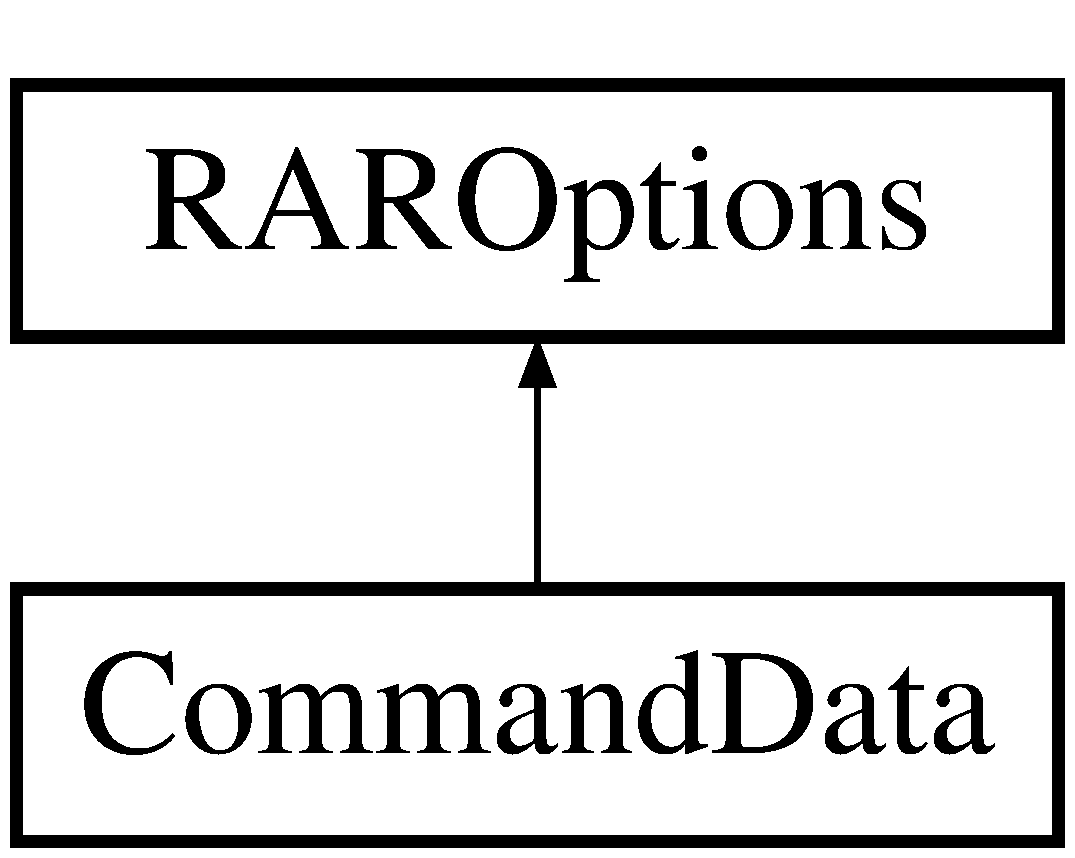
\includegraphics[height=2.000000cm]{class_r_a_r_options}
\end{center}
\end{figure}
\subsection*{Public Member Functions}
\begin{DoxyCompactItemize}
\item 
\hypertarget{class_r_a_r_options_ae403dd553c8755ce1bce25455c9f47b2}{void {\bfseries Init} ()}\label{class_r_a_r_options_ae403dd553c8755ce1bce25455c9f47b2}

\end{DoxyCompactItemize}
\subsection*{Public Attributes}
\begin{DoxyCompactItemize}
\item 
\hypertarget{class_r_a_r_options_ac4fd3ae92e02a8dba3a55c3e259f17d1}{uint {\bfseries Excl\-File\-Attr}}\label{class_r_a_r_options_ac4fd3ae92e02a8dba3a55c3e259f17d1}

\item 
\hypertarget{class_r_a_r_options_aa895c5e88b4311246c555b903c93c4fb}{uint {\bfseries Incl\-File\-Attr}}\label{class_r_a_r_options_aa895c5e88b4311246c555b903c93c4fb}

\item 
\hypertarget{class_r_a_r_options_ae422103f3421d5c7a3dba1cbeb76717c}{bool {\bfseries Incl\-Attr\-Set}}\label{class_r_a_r_options_ae422103f3421d5c7a3dba1cbeb76717c}

\item 
\hypertarget{class_r_a_r_options_a537e09b75eeba47ea3495e8276753233}{uint {\bfseries Win\-Size}}\label{class_r_a_r_options_a537e09b75eeba47ea3495e8276753233}

\item 
\hypertarget{class_r_a_r_options_a91f9d4a53e851fe40bceeba768cb7cd8}{char {\bfseries Temp\-Path} \mbox{[}N\-M\mbox{]}}\label{class_r_a_r_options_a91f9d4a53e851fe40bceeba768cb7cd8}

\item 
\hypertarget{class_r_a_r_options_a86d863ff4bf7bfa2a8e71c394e2c5c26}{bool {\bfseries Config\-Disabled}}\label{class_r_a_r_options_a86d863ff4bf7bfa2a8e71c394e2c5c26}

\item 
\hypertarget{class_r_a_r_options_a9a4b8705cab34c0c6f85cf739e970455}{char {\bfseries Extr\-Path} \mbox{[}N\-M\mbox{]}}\label{class_r_a_r_options_a9a4b8705cab34c0c6f85cf739e970455}

\item 
\hypertarget{class_r_a_r_options_aaee6f00c1ddcbc24c221ddbb76e035a5}{wchar {\bfseries Extr\-Path\-W} \mbox{[}N\-M\mbox{]}}\label{class_r_a_r_options_aaee6f00c1ddcbc24c221ddbb76e035a5}

\item 
\hypertarget{class_r_a_r_options_aeede75378e7dbf06c97b3950ff8fa2a2}{char {\bfseries Comment\-File} \mbox{[}N\-M\mbox{]}}\label{class_r_a_r_options_aeede75378e7dbf06c97b3950ff8fa2a2}

\item 
\hypertarget{class_r_a_r_options_ad9463beb4e47273b8c12567258aa038d}{wchar {\bfseries Comment\-File\-W} \mbox{[}N\-M\mbox{]}}\label{class_r_a_r_options_ad9463beb4e47273b8c12567258aa038d}

\item 
\hypertarget{class_r_a_r_options_a3307898d95639c3dd7fbeaa83c7e5087}{R\-A\-R\-\_\-\-C\-H\-A\-R\-S\-E\-T {\bfseries Comment\-Charset}}\label{class_r_a_r_options_a3307898d95639c3dd7fbeaa83c7e5087}

\item 
\hypertarget{class_r_a_r_options_a6b716132e1ed8c4f68d47c3012ec5af3}{R\-A\-R\-\_\-\-C\-H\-A\-R\-S\-E\-T {\bfseries Filelist\-Charset}}\label{class_r_a_r_options_a6b716132e1ed8c4f68d47c3012ec5af3}

\item 
\hypertarget{class_r_a_r_options_add6a48c8149fbbd8f59171b4e318b214}{char {\bfseries Arc\-Path} \mbox{[}N\-M\mbox{]}}\label{class_r_a_r_options_add6a48c8149fbbd8f59171b4e318b214}

\item 
\hypertarget{class_r_a_r_options_ae7104f0d402049b8dd8de38de05d8495}{wchar {\bfseries Arc\-Path\-W} \mbox{[}N\-M\mbox{]}}\label{class_r_a_r_options_ae7104f0d402049b8dd8de38de05d8495}

\item 
\hypertarget{class_r_a_r_options_a0da0b89cf7532c6ef3c58b7abb8a53a8}{wchar {\bfseries Password} \mbox{[}M\-A\-X\-P\-A\-S\-S\-W\-O\-R\-D\mbox{]}}\label{class_r_a_r_options_a0da0b89cf7532c6ef3c58b7abb8a53a8}

\item 
\hypertarget{class_r_a_r_options_a0d55adc2842352e589293af369647a34}{bool {\bfseries Encrypt\-Headers}}\label{class_r_a_r_options_a0d55adc2842352e589293af369647a34}

\item 
\hypertarget{class_r_a_r_options_acb0f8cbd6f3ea9c3e4a2ceb5035bed9a}{char {\bfseries Log\-Name} \mbox{[}N\-M\mbox{]}}\label{class_r_a_r_options_acb0f8cbd6f3ea9c3e4a2ceb5035bed9a}

\item 
\hypertarget{class_r_a_r_options_ac49e1e7a90d776ef7b72cf690b3111e0}{M\-E\-S\-S\-A\-G\-E\-\_\-\-T\-Y\-P\-E {\bfseries Msg\-Stream}}\label{class_r_a_r_options_ac49e1e7a90d776ef7b72cf690b3111e0}

\item 
\hypertarget{class_r_a_r_options_a24cab6602929abe4a40b9b5204070213}{bool {\bfseries Sound}}\label{class_r_a_r_options_a24cab6602929abe4a40b9b5204070213}

\item 
\hypertarget{class_r_a_r_options_aee09874844e17d9930dfc47b95d10061}{O\-V\-E\-R\-W\-R\-I\-T\-E\-\_\-\-M\-O\-D\-E {\bfseries Overwrite}}\label{class_r_a_r_options_aee09874844e17d9930dfc47b95d10061}

\item 
\hypertarget{class_r_a_r_options_ab653aef55c72c6ab5bced72c4081aa6a}{int {\bfseries Method}}\label{class_r_a_r_options_ab653aef55c72c6ab5bced72c4081aa6a}

\item 
\hypertarget{class_r_a_r_options_a894ec15f1990f80477341ca2d06ed87b}{int {\bfseries Recovery}}\label{class_r_a_r_options_a894ec15f1990f80477341ca2d06ed87b}

\item 
\hypertarget{class_r_a_r_options_afba8be1f5b1ed1ebd4fa85f8c3cab47a}{int {\bfseries Rec\-Vol\-Number}}\label{class_r_a_r_options_afba8be1f5b1ed1ebd4fa85f8c3cab47a}

\item 
\hypertarget{class_r_a_r_options_ac8b9ee1de7f6562875f77dff862c33ed}{bool {\bfseries Disable\-Percentage}}\label{class_r_a_r_options_ac8b9ee1de7f6562875f77dff862c33ed}

\item 
\hypertarget{class_r_a_r_options_a82916432f9c1021338825f8583d011fb}{bool {\bfseries Disable\-Copyright}}\label{class_r_a_r_options_a82916432f9c1021338825f8583d011fb}

\item 
\hypertarget{class_r_a_r_options_abd2e900547898faaf2026f9b0e73b182}{bool {\bfseries Disable\-Done}}\label{class_r_a_r_options_abd2e900547898faaf2026f9b0e73b182}

\item 
\hypertarget{class_r_a_r_options_a8377d90af5a75b890b5578c33604f9db}{int {\bfseries Solid}}\label{class_r_a_r_options_a8377d90af5a75b890b5578c33604f9db}

\item 
\hypertarget{class_r_a_r_options_a6e2826f2f8a8a1a51eb044965a8706b2}{int {\bfseries Solid\-Count}}\label{class_r_a_r_options_a6e2826f2f8a8a1a51eb044965a8706b2}

\item 
\hypertarget{class_r_a_r_options_abcb1c92e1ec66b2ed37025bb4803cc18}{bool {\bfseries Clear\-Arc}}\label{class_r_a_r_options_abcb1c92e1ec66b2ed37025bb4803cc18}

\item 
\hypertarget{class_r_a_r_options_a010a02be4f2a79abb922ddf1406c6a52}{bool {\bfseries Add\-Arc\-Only}}\label{class_r_a_r_options_a010a02be4f2a79abb922ddf1406c6a52}

\item 
\hypertarget{class_r_a_r_options_ae5c3f88ec7dd9c7e69ce2162fccf467a}{bool {\bfseries A\-V}}\label{class_r_a_r_options_ae5c3f88ec7dd9c7e69ce2162fccf467a}

\item 
\hypertarget{class_r_a_r_options_aca59e4f3ced70c5998267d14ad5a7543}{bool {\bfseries Disable\-Comment}}\label{class_r_a_r_options_aca59e4f3ced70c5998267d14ad5a7543}

\item 
\hypertarget{class_r_a_r_options_a14789773a7b42747fcaddbb5cdf082d0}{bool {\bfseries Fresh\-Files}}\label{class_r_a_r_options_a14789773a7b42747fcaddbb5cdf082d0}

\item 
\hypertarget{class_r_a_r_options_a3f97f9f5fcd050005b197d015e5c81d2}{bool {\bfseries Update\-Files}}\label{class_r_a_r_options_a3f97f9f5fcd050005b197d015e5c81d2}

\item 
\hypertarget{class_r_a_r_options_aa33417978226f9776cb9963100b6a452}{P\-A\-T\-H\-\_\-\-E\-X\-C\-L\-\_\-\-M\-O\-D\-E {\bfseries Excl\-Path}}\label{class_r_a_r_options_aa33417978226f9776cb9963100b6a452}

\item 
\hypertarget{class_r_a_r_options_a4848b9b7d4923c3e570d32b1fa907d57}{R\-E\-C\-U\-R\-S\-E\-\_\-\-M\-O\-D\-E {\bfseries Recurse}}\label{class_r_a_r_options_a4848b9b7d4923c3e570d32b1fa907d57}

\item 
\hypertarget{class_r_a_r_options_a72ae32013919152040b19f58789b8e2b}{int64 {\bfseries Vol\-Size}}\label{class_r_a_r_options_a72ae32013919152040b19f58789b8e2b}

\item 
\hypertarget{class_r_a_r_options_a5fe509d138e9b7b9001d4ecb680f0ac7}{\hyperlink{class_array}{Array}$<$ int64 $>$ {\bfseries Next\-Vol\-Sizes}}\label{class_r_a_r_options_a5fe509d138e9b7b9001d4ecb680f0ac7}

\item 
\hypertarget{class_r_a_r_options_aee3bf13e6af9edf43d3c42bf9c50e59d}{uint {\bfseries Cur\-Vol\-Num}}\label{class_r_a_r_options_aee3bf13e6af9edf43d3c42bf9c50e59d}

\item 
\hypertarget{class_r_a_r_options_a48bb8e391f17281cf5cfdba57341f005}{bool {\bfseries All\-Yes}}\label{class_r_a_r_options_a48bb8e391f17281cf5cfdba57341f005}

\item 
\hypertarget{class_r_a_r_options_a2c26ae6170bb5199a6d3db4d4fe6af8f}{bool {\bfseries Disable\-View\-A\-V}}\label{class_r_a_r_options_a2c26ae6170bb5199a6d3db4d4fe6af8f}

\item 
\hypertarget{class_r_a_r_options_a4a89504a41d4f8f95a61f65654b5b2cd}{bool {\bfseries Disable\-Sort\-Solid}}\label{class_r_a_r_options_a4a89504a41d4f8f95a61f65654b5b2cd}

\item 
\hypertarget{class_r_a_r_options_ab3d5c7b3e8248161088c61c1f7197a4b}{int {\bfseries Arc\-Time}}\label{class_r_a_r_options_ab3d5c7b3e8248161088c61c1f7197a4b}

\item 
\hypertarget{class_r_a_r_options_ac6251311478e5480ebd3c38faa439a86}{int {\bfseries Convert\-Names}}\label{class_r_a_r_options_ac6251311478e5480ebd3c38faa439a86}

\item 
\hypertarget{class_r_a_r_options_aa37cecd8162d64513b95637f6ec482f4}{bool {\bfseries Process\-Owners}}\label{class_r_a_r_options_aa37cecd8162d64513b95637f6ec482f4}

\item 
\hypertarget{class_r_a_r_options_a568f370a5ea021fc0c3bfb7a2903c5fa}{bool {\bfseries Save\-Links}}\label{class_r_a_r_options_a568f370a5ea021fc0c3bfb7a2903c5fa}

\item 
\hypertarget{class_r_a_r_options_a4397b4c137b9c2c15f7a567d10843a83}{int {\bfseries Priority}}\label{class_r_a_r_options_a4397b4c137b9c2c15f7a567d10843a83}

\item 
\hypertarget{class_r_a_r_options_aa7e7d80585f353c8d1e0e50946ce928e}{int {\bfseries Sleep\-Time}}\label{class_r_a_r_options_aa7e7d80585f353c8d1e0e50946ce928e}

\item 
\hypertarget{class_r_a_r_options_a4ca15ca12aed1f3b1466d5f70bbc49c6}{bool {\bfseries Keep\-Broken}}\label{class_r_a_r_options_a4ca15ca12aed1f3b1466d5f70bbc49c6}

\item 
\hypertarget{class_r_a_r_options_ad71b222373cb6e44d4d728f0d17f6b23}{bool {\bfseries Open\-Shared}}\label{class_r_a_r_options_ad71b222373cb6e44d4d728f0d17f6b23}

\item 
\hypertarget{class_r_a_r_options_affaac2325dce4ced95f1fefe8fb986ac}{bool {\bfseries Delete\-Files}}\label{class_r_a_r_options_affaac2325dce4ced95f1fefe8fb986ac}

\item 
\hypertarget{class_r_a_r_options_a40317089149416e9a63cf385dc70f099}{bool {\bfseries Generate\-Arc\-Name}}\label{class_r_a_r_options_a40317089149416e9a63cf385dc70f099}

\item 
\hypertarget{class_r_a_r_options_ad48e9c2da43dd5337efde4e34422f116}{char {\bfseries Generate\-Mask} \mbox{[}M\-A\-X\-\_\-\-G\-E\-N\-E\-R\-A\-T\-E\-\_\-\-M\-A\-S\-K\mbox{]}}\label{class_r_a_r_options_ad48e9c2da43dd5337efde4e34422f116}

\item 
\hypertarget{class_r_a_r_options_aa8b417b1964d114afb8886963559eeb9}{bool {\bfseries Sync\-Files}}\label{class_r_a_r_options_aa8b417b1964d114afb8886963559eeb9}

\item 
\hypertarget{class_r_a_r_options_aec313e7dbd2ff4e1b42c3110b3495a56}{bool {\bfseries Process\-E\-A}}\label{class_r_a_r_options_aec313e7dbd2ff4e1b42c3110b3495a56}

\item 
\hypertarget{class_r_a_r_options_abf8d622e20e7b3f00c9701f75d91a8f0}{bool {\bfseries Save\-Streams}}\label{class_r_a_r_options_abf8d622e20e7b3f00c9701f75d91a8f0}

\item 
\hypertarget{class_r_a_r_options_a119c3240e25ca12ec55cf1372591ed58}{bool {\bfseries Set\-Compressed\-Attr}}\label{class_r_a_r_options_a119c3240e25ca12ec55cf1372591ed58}

\item 
\hypertarget{class_r_a_r_options_a19438903d025935c5843cce9895eaad4}{bool {\bfseries Ignore\-General\-Attr}}\label{class_r_a_r_options_a19438903d025935c5843cce9895eaad4}

\item 
\hypertarget{class_r_a_r_options_a062533a916678ea9b81a88f1b0b5320d}{\hyperlink{class_rar_time}{Rar\-Time} {\bfseries File\-Time\-Before}}\label{class_r_a_r_options_a062533a916678ea9b81a88f1b0b5320d}

\item 
\hypertarget{class_r_a_r_options_a541dbd2acc25dbf4bb32015c89021e3a}{\hyperlink{class_rar_time}{Rar\-Time} {\bfseries File\-Time\-After}}\label{class_r_a_r_options_a541dbd2acc25dbf4bb32015c89021e3a}

\item 
\hypertarget{class_r_a_r_options_aca5b218cd57a6845caacb6d531e3b340}{int64 {\bfseries File\-Size\-Less}}\label{class_r_a_r_options_aca5b218cd57a6845caacb6d531e3b340}

\item 
\hypertarget{class_r_a_r_options_ae463ac6466dd031f99a03b8124cf6559}{int64 {\bfseries File\-Size\-More}}\label{class_r_a_r_options_ae463ac6466dd031f99a03b8124cf6559}

\item 
\hypertarget{class_r_a_r_options_a37452789da68800f70d552de623d2921}{bool {\bfseries Old\-Numbering}}\label{class_r_a_r_options_a37452789da68800f70d552de623d2921}

\item 
\hypertarget{class_r_a_r_options_aca02068c25f64c32e7eb677cf1560bbf}{bool {\bfseries Lock}}\label{class_r_a_r_options_aca02068c25f64c32e7eb677cf1560bbf}

\item 
\hypertarget{class_r_a_r_options_ad50969d316601f42fc2f74ac52f093e9}{bool {\bfseries Test}}\label{class_r_a_r_options_ad50969d316601f42fc2f74ac52f093e9}

\item 
\hypertarget{class_r_a_r_options_a0f8d1e8989441c929ec92ed304f2876a}{bool {\bfseries Volume\-Pause}}\label{class_r_a_r_options_a0f8d1e8989441c929ec92ed304f2876a}

\item 
\hypertarget{class_r_a_r_options_aa7bfad6f9becd063848c1431f6bcf654}{\hyperlink{struct_filter_mode}{Filter\-Mode} {\bfseries Filter\-Modes} \mbox{[}M\-A\-X\-\_\-\-F\-I\-L\-T\-E\-R\-S\mbox{]}}\label{class_r_a_r_options_aa7bfad6f9becd063848c1431f6bcf654}

\item 
\hypertarget{class_r_a_r_options_a52eba8e766200200a8af6b711e4b7929}{char {\bfseries Email\-To} \mbox{[}N\-M\mbox{]}}\label{class_r_a_r_options_a52eba8e766200200a8af6b711e4b7929}

\item 
\hypertarget{class_r_a_r_options_acd4940bd4fe84ff26444c2f5fad5d5bb}{uint {\bfseries Version\-Control}}\label{class_r_a_r_options_acd4940bd4fe84ff26444c2f5fad5d5bb}

\item 
\hypertarget{class_r_a_r_options_af68d3deb81260eb013ec986632655c02}{bool {\bfseries No\-End\-Block}}\label{class_r_a_r_options_af68d3deb81260eb013ec986632655c02}

\item 
\hypertarget{class_r_a_r_options_a6ac1a458fc60872fdb5d7f7003d0ec37}{bool {\bfseries Append\-Arc\-Name\-To\-Path}}\label{class_r_a_r_options_a6ac1a458fc60872fdb5d7f7003d0ec37}

\item 
\hypertarget{class_r_a_r_options_a3de54f7ef0a722cec1a44802595bf5dd}{bool {\bfseries Shutdown}}\label{class_r_a_r_options_a3de54f7ef0a722cec1a44802595bf5dd}

\item 
\hypertarget{class_r_a_r_options_a8e73d96b8920136dcfed7ae3574da95b}{E\-X\-T\-T\-I\-M\-E\-\_\-\-M\-O\-D\-E {\bfseries xmtime}}\label{class_r_a_r_options_a8e73d96b8920136dcfed7ae3574da95b}

\item 
\hypertarget{class_r_a_r_options_afd896e1aaadf3fb7cc2a3e1e2dcef1aa}{E\-X\-T\-T\-I\-M\-E\-\_\-\-M\-O\-D\-E {\bfseries xctime}}\label{class_r_a_r_options_afd896e1aaadf3fb7cc2a3e1e2dcef1aa}

\item 
\hypertarget{class_r_a_r_options_a9c060d821fb807b485a89eec13262491}{E\-X\-T\-T\-I\-M\-E\-\_\-\-M\-O\-D\-E {\bfseries xatime}}\label{class_r_a_r_options_a9c060d821fb807b485a89eec13262491}

\item 
\hypertarget{class_r_a_r_options_a27eb05a796e2b9e116cfed595506774d}{E\-X\-T\-T\-I\-M\-E\-\_\-\-M\-O\-D\-E {\bfseries xarctime}}\label{class_r_a_r_options_a27eb05a796e2b9e116cfed595506774d}

\item 
\hypertarget{class_r_a_r_options_a864f7f7e237f708294361ed156763bf8}{char {\bfseries Compress\-Stdin} \mbox{[}N\-M\mbox{]}}\label{class_r_a_r_options_a864f7f7e237f708294361ed156763bf8}

\end{DoxyCompactItemize}


The documentation for this class was generated from the following files\-:\begin{DoxyCompactItemize}
\item 
/\-Users/salazbr1/\-Documents/\-N\-P\-S/final\-\_\-unrarbulk\-\_\-extractor\-\_\-07-\/26-\/12/code/options.\-hpp\item 
/\-Users/salazbr1/\-Documents/\-N\-P\-S/final\-\_\-unrarbulk\-\_\-extractor\-\_\-07-\/26-\/12/code/options.\-cpp\end{DoxyCompactItemize}

\hypertarget{class_rar_time}{\section{Rar\-Time Class Reference}
\label{class_rar_time}\index{Rar\-Time@{Rar\-Time}}
}
\subsection*{Public Member Functions}
\begin{DoxyCompactItemize}
\item 
\hypertarget{class_rar_time_a660243101164121b76f080b230ecf0d0}{bool {\bfseries operator==} (\hyperlink{class_rar_time}{Rar\-Time} \&rt)}\label{class_rar_time_a660243101164121b76f080b230ecf0d0}

\item 
\hypertarget{class_rar_time_aa3899980120b9d0bf62c821055a23bd7}{bool {\bfseries operator$<$} (\hyperlink{class_rar_time}{Rar\-Time} \&rt)}\label{class_rar_time_aa3899980120b9d0bf62c821055a23bd7}

\item 
\hypertarget{class_rar_time_a3b9c924a1ab108050bcbc0cb1ee2c22f}{bool {\bfseries operator$<$=} (\hyperlink{class_rar_time}{Rar\-Time} \&rt)}\label{class_rar_time_a3b9c924a1ab108050bcbc0cb1ee2c22f}

\item 
\hypertarget{class_rar_time_ad0ce18c2c9bfade4bdfa8a1861e3195d}{bool {\bfseries operator$>$} (\hyperlink{class_rar_time}{Rar\-Time} \&rt)}\label{class_rar_time_ad0ce18c2c9bfade4bdfa8a1861e3195d}

\item 
\hypertarget{class_rar_time_af844636bf6bf5fc32e9907777fdf4037}{bool {\bfseries operator$>$=} (\hyperlink{class_rar_time}{Rar\-Time} \&rt)}\label{class_rar_time_af844636bf6bf5fc32e9907777fdf4037}

\item 
\hypertarget{class_rar_time_a1c9eea16d7ead475734909e4ac75d5c1}{void {\bfseries Get\-Local} (\hyperlink{struct_rar_local_time}{Rar\-Local\-Time} $\ast$lt)}\label{class_rar_time_a1c9eea16d7ead475734909e4ac75d5c1}

\item 
\hypertarget{class_rar_time_af4bd79179dc9f29beccbc22e9e4f036c}{void {\bfseries Set\-Local} (\hyperlink{struct_rar_local_time}{Rar\-Local\-Time} $\ast$lt)}\label{class_rar_time_af4bd79179dc9f29beccbc22e9e4f036c}

\item 
\hypertarget{class_rar_time_a12782cfa1d6c200d9ca69f7f7ee643d3}{int64 {\bfseries Get\-Raw} ()}\label{class_rar_time_a12782cfa1d6c200d9ca69f7f7ee643d3}

\item 
\hypertarget{class_rar_time_a1879a1d3091c0ecb6865628b18564893}{void {\bfseries Set\-Raw} (int64 Raw\-Time)}\label{class_rar_time_a1879a1d3091c0ecb6865628b18564893}

\item 
\hypertarget{class_rar_time_a18a4f91d384feacefdbd2ceaa2964c55}{uint {\bfseries Get\-Dos} ()}\label{class_rar_time_a18a4f91d384feacefdbd2ceaa2964c55}

\item 
\hypertarget{class_rar_time_a0efa4b519c13394dd086e504a97085af}{void {\bfseries Set\-Dos} (uint Dos\-Time)}\label{class_rar_time_a0efa4b519c13394dd086e504a97085af}

\item 
\hypertarget{class_rar_time_a536860b5c8756ee0ff116cfe806ea5e3}{void {\bfseries Get\-Text} (char $\ast$Date\-Str, bool Full\-Year)}\label{class_rar_time_a536860b5c8756ee0ff116cfe806ea5e3}

\item 
\hypertarget{class_rar_time_a7d4133c5503560774d5be549f4549d7b}{void {\bfseries Set\-Iso\-Text} (const char $\ast$Time\-Text)}\label{class_rar_time_a7d4133c5503560774d5be549f4549d7b}

\item 
\hypertarget{class_rar_time_ab17a77662ab8d2961f85c2a0cb21aedb}{void {\bfseries Set\-Age\-Text} (const char $\ast$Time\-Text)}\label{class_rar_time_ab17a77662ab8d2961f85c2a0cb21aedb}

\item 
\hypertarget{class_rar_time_ac177f261789384edae956b3376903909}{void {\bfseries Set\-Current\-Time} ()}\label{class_rar_time_ac177f261789384edae956b3376903909}

\item 
\hypertarget{class_rar_time_a3faa4008398f4abe68294e9a113ca13c}{std\-::string {\bfseries Get\-Local\-Time\-X\-M\-L} ()}\label{class_rar_time_a3faa4008398f4abe68294e9a113ca13c}

\item 
\hypertarget{class_rar_time_af6064bc1f013b99b24f7931010483b08}{void {\bfseries Reset} ()}\label{class_rar_time_af6064bc1f013b99b24f7931010483b08}

\item 
\hypertarget{class_rar_time_addffbeddff095f118c0cd6121d408087}{bool {\bfseries Is\-Set} ()}\label{class_rar_time_addffbeddff095f118c0cd6121d408087}

\end{DoxyCompactItemize}


The documentation for this class was generated from the following files\-:\begin{DoxyCompactItemize}
\item 
/\-Users/salazbr1/\-Documents/\-N\-P\-S/final\-\_\-unrarbulk\-\_\-extractor\-\_\-07-\/26-\/12/code/timefn.\-hpp\item 
/\-Users/salazbr1/\-Documents/\-N\-P\-S/final\-\_\-unrarbulk\-\_\-extractor\-\_\-07-\/26-\/12/code/timefn.\-cpp\end{DoxyCompactItemize}

\hypertarget{class_rar_v_m}{\section{Rar\-V\-M Class Reference}
\label{class_rar_v_m}\index{Rar\-V\-M@{Rar\-V\-M}}
}
Inheritance diagram for Rar\-V\-M\-:\begin{figure}[H]
\begin{center}
\leavevmode
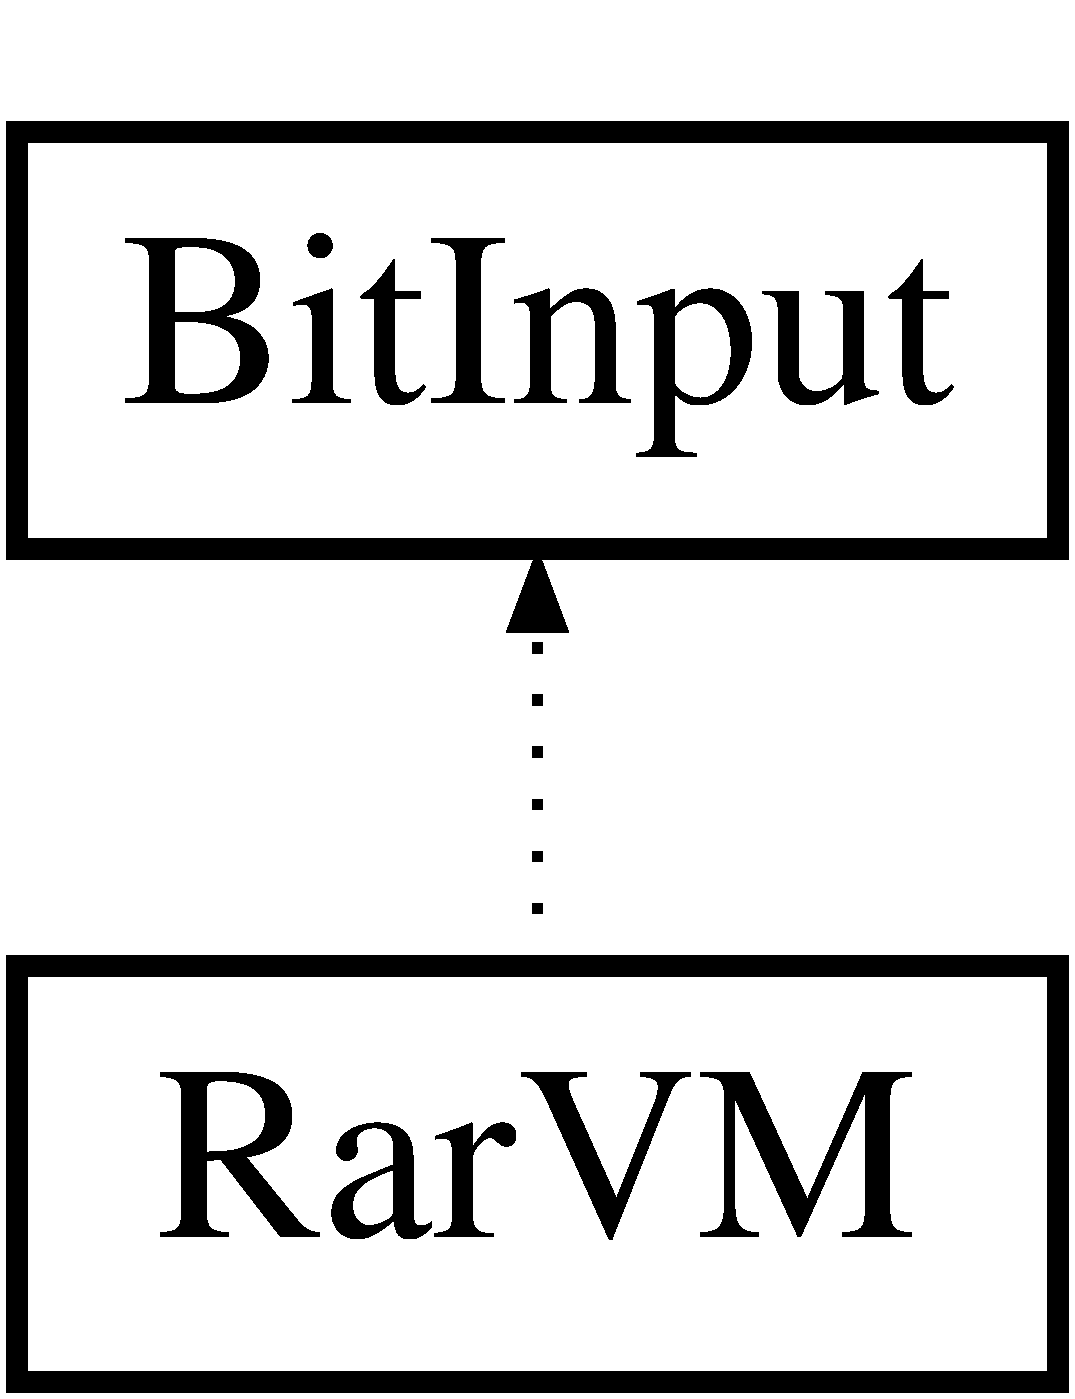
\includegraphics[height=2.000000cm]{class_rar_v_m}
\end{center}
\end{figure}
\subsection*{Public Member Functions}
\begin{DoxyCompactItemize}
\item 
\hypertarget{class_rar_v_m_afa9d20c695b5f81ac34d0ca5fd4b1a08}{void {\bfseries Init} ()}\label{class_rar_v_m_afa9d20c695b5f81ac34d0ca5fd4b1a08}

\item 
\hypertarget{class_rar_v_m_a2ed25f5389962c5afd93ccf6fb54d836}{void {\bfseries Prepare} (byte $\ast$Code, uint Code\-Size, \hyperlink{struct_v_m___prepared_program}{V\-M\-\_\-\-Prepared\-Program} $\ast$Prg)}\label{class_rar_v_m_a2ed25f5389962c5afd93ccf6fb54d836}

\item 
\hypertarget{class_rar_v_m_a2485c5618eadfab809c96a2383634dab}{void {\bfseries Execute} (\hyperlink{struct_v_m___prepared_program}{V\-M\-\_\-\-Prepared\-Program} $\ast$Prg)}\label{class_rar_v_m_a2485c5618eadfab809c96a2383634dab}

\item 
\hypertarget{class_rar_v_m_aa7fa8bd5e413e7ae1c9c886e153825e6}{void {\bfseries Set\-Low\-Endian\-Value} (uint $\ast$Addr, uint Value)}\label{class_rar_v_m_aa7fa8bd5e413e7ae1c9c886e153825e6}

\item 
\hypertarget{class_rar_v_m_a98b627565c534ab38e6ea0879252d381}{void {\bfseries Set\-Memory} (uint Pos, byte $\ast$Data, uint Data\-Size)}\label{class_rar_v_m_a98b627565c534ab38e6ea0879252d381}

\end{DoxyCompactItemize}
\subsection*{Static Public Member Functions}
\begin{DoxyCompactItemize}
\item 
\hypertarget{class_rar_v_m_a6eb3a8147b369f1e3b22adb796cbd94c}{static uint {\bfseries Read\-Data} (\hyperlink{class_bit_input}{Bit\-Input} \&Inp)}\label{class_rar_v_m_a6eb3a8147b369f1e3b22adb796cbd94c}

\end{DoxyCompactItemize}
\subsection*{Additional Inherited Members}


The documentation for this class was generated from the following files\-:\begin{DoxyCompactItemize}
\item 
/\-Users/salazbr1/\-Documents/\-N\-P\-S/final\-\_\-unrarbulk\-\_\-extractor\-\_\-07-\/26-\/12/code/rarvm.\-hpp\item 
/\-Users/salazbr1/\-Documents/\-N\-P\-S/final\-\_\-unrarbulk\-\_\-extractor\-\_\-07-\/26-\/12/code/rarvm.\-cpp\end{DoxyCompactItemize}

\hypertarget{class_raw_read}{\section{Raw\-Read Class Reference}
\label{class_raw_read}\index{Raw\-Read@{Raw\-Read}}
}


{\ttfamily \#include $<$rawread.\-hpp$>$}

\subsection*{Public Member Functions}
\begin{DoxyCompactItemize}
\item 
\hyperlink{class_raw_read_a1a9f297d8dd914ac067267bb9e4ce589}{Raw\-Read} (\hyperlink{class_file}{File} $\ast$Src\-File)
\item 
\hypertarget{class_raw_read_a0ed3fce8f38f950d45da36736b520520}{void {\bfseries Read} (size\-\_\-t Size)}\label{class_raw_read_a0ed3fce8f38f950d45da36736b520520}

\item 
\hypertarget{class_raw_read_a6c5aa71f05a102004a102adcafbb8a5c}{void {\bfseries Read} (byte $\ast$Src\-Data, size\-\_\-t Size)}\label{class_raw_read_a6c5aa71f05a102004a102adcafbb8a5c}

\item 
\hypertarget{class_raw_read_ac74d0439fc0203119332e6df19683c85}{void {\bfseries Get} (byte \&Field)}\label{class_raw_read_ac74d0439fc0203119332e6df19683c85}

\item 
\hypertarget{class_raw_read_a5ad89c0e6831687b144b4d5f4610f608}{void {\bfseries Get} (ushort \&Field)}\label{class_raw_read_a5ad89c0e6831687b144b4d5f4610f608}

\item 
\hypertarget{class_raw_read_abdf916d71c4e85b03fb525d88fafb9ce}{void {\bfseries Get} (uint \&Field)}\label{class_raw_read_abdf916d71c4e85b03fb525d88fafb9ce}

\item 
\hypertarget{class_raw_read_a0d114615c5830333b07d2a3893f7d647}{void {\bfseries Get8} (int64 \&Field)}\label{class_raw_read_a0d114615c5830333b07d2a3893f7d647}

\item 
\hypertarget{class_raw_read_ab38e81db925883b02c70e86166727cc5}{void {\bfseries Get} (byte $\ast$Field, size\-\_\-t Size)}\label{class_raw_read_ab38e81db925883b02c70e86166727cc5}

\item 
\hypertarget{class_raw_read_a6ec2600a08850e0100a22051278c3567}{void {\bfseries Get} (wchar $\ast$Field, size\-\_\-t Size)}\label{class_raw_read_a6ec2600a08850e0100a22051278c3567}

\item 
\hypertarget{class_raw_read_aff8ec67ee8b25467fa2dc00d2d626782}{uint {\bfseries Get\-C\-R\-C} (bool Processed\-Only)}\label{class_raw_read_aff8ec67ee8b25467fa2dc00d2d626782}

\item 
\hypertarget{class_raw_read_aacda1b22635f98246205f6a3c4660324}{size\-\_\-t {\bfseries Size} ()}\label{class_raw_read_aacda1b22635f98246205f6a3c4660324}

\item 
\hypertarget{class_raw_read_adf9af01beb1b80ea5f910cef586cf979}{size\-\_\-t {\bfseries Padded\-Size} ()}\label{class_raw_read_adf9af01beb1b80ea5f910cef586cf979}

\item 
\hypertarget{class_raw_read_a518fa936b7bbfc66c395c85127f1bfa7}{void {\bfseries Set\-Crypt} (\hyperlink{class_crypt_data}{Crypt\-Data} $\ast$Crypt)}\label{class_raw_read_a518fa936b7bbfc66c395c85127f1bfa7}

\end{DoxyCompactItemize}


\subsection{Detailed Description}
This class performs different types of read functions from the {\ttfamily \hyperlink{class_file}{File}} class The functions should be self-\/explanatory. 

\subsection{Constructor \& Destructor Documentation}
\hypertarget{class_raw_read_a1a9f297d8dd914ac067267bb9e4ce589}{\index{Raw\-Read@{Raw\-Read}!Raw\-Read@{Raw\-Read}}
\index{Raw\-Read@{Raw\-Read}!RawRead@{Raw\-Read}}
\subsubsection[{Raw\-Read}]{\setlength{\rightskip}{0pt plus 5cm}Raw\-Read\-::\-Raw\-Read (
\begin{DoxyParamCaption}
\item[{{\bf File} $\ast$}]{Src\-File}
\end{DoxyParamCaption}
)}}\label{class_raw_read_a1a9f297d8dd914ac067267bb9e4ce589}
Constructor function for the {\ttfamily \hyperlink{class_raw_read}{Raw\-Read}} class 
\begin{DoxyParams}{Parameters}
{\em Src\-File} & -\/ the {\ttfamily \hyperlink{class_file}{File}} object that this class will read from \\
\hline
\end{DoxyParams}


The documentation for this class was generated from the following files\-:\begin{DoxyCompactItemize}
\item 
/\-Users/salazbr1/\-Documents/\-N\-P\-S/final\-\_\-unrarbulk\-\_\-extractor\-\_\-07-\/26-\/12/code/rawread.\-hpp\item 
/\-Users/salazbr1/\-Documents/\-N\-P\-S/final\-\_\-unrarbulk\-\_\-extractor\-\_\-07-\/26-\/12/code/rawread.\-cpp\end{DoxyCompactItemize}

\hypertarget{class_rec_volumes}{\section{Rec\-Volumes Class Reference}
\label{class_rec_volumes}\index{Rec\-Volumes@{Rec\-Volumes}}
}
\subsection*{Public Member Functions}
\begin{DoxyCompactItemize}
\item 
\hypertarget{class_rec_volumes_a4c67e0e29250ea3383f594ac8b31e22f}{void {\bfseries Make} (\hyperlink{class_r_a_r_options}{R\-A\-R\-Options} $\ast$Cmd, char $\ast$Arc\-Name, wchar $\ast$Arc\-Name\-W)}\label{class_rec_volumes_a4c67e0e29250ea3383f594ac8b31e22f}

\item 
\hypertarget{class_rec_volumes_ad4fdf3ecc57f619ea464fe9ce0bc5e27}{bool {\bfseries Restore} (\hyperlink{class_r_a_r_options}{R\-A\-R\-Options} $\ast$Cmd, const char $\ast$Name, const wchar $\ast$Name\-W, bool Silent)}\label{class_rec_volumes_ad4fdf3ecc57f619ea464fe9ce0bc5e27}

\end{DoxyCompactItemize}


The documentation for this class was generated from the following files\-:\begin{DoxyCompactItemize}
\item 
/\-Users/salazbr1/\-Documents/\-N\-P\-S/final\-\_\-unrarbulk\-\_\-extractor\-\_\-07-\/26-\/12/code/recvol.\-hpp\item 
/\-Users/salazbr1/\-Documents/\-N\-P\-S/final\-\_\-unrarbulk\-\_\-extractor\-\_\-07-\/26-\/12/code/recvol.\-cpp\end{DoxyCompactItemize}

\hypertarget{class_rijndael}{\section{Rijndael Class Reference}
\label{class_rijndael}\index{Rijndael@{Rijndael}}
}
\subsection*{Public Types}
\begin{DoxyCompactItemize}
\item 
enum {\bfseries Direction} \{ {\bfseries Encrypt}, 
{\bfseries Decrypt}
 \}
\end{DoxyCompactItemize}
\subsection*{Public Member Functions}
\begin{DoxyCompactItemize}
\item 
\hypertarget{class_rijndael_a4f07601b925a7eff472e4e2dc4ee1f06}{void {\bfseries init} (Direction dir, const byte $\ast$key, byte $\ast$init\-Vector)}\label{class_rijndael_a4f07601b925a7eff472e4e2dc4ee1f06}

\item 
\hypertarget{class_rijndael_ac105e87a43362d92865565c27a2c509d}{size\-\_\-t {\bfseries block\-Encrypt} (const byte $\ast$input, size\-\_\-t input\-Len, byte $\ast$out\-Buffer)}\label{class_rijndael_ac105e87a43362d92865565c27a2c509d}

\item 
\hypertarget{class_rijndael_a3104a56aacfd053262f845fede98d4b6}{size\-\_\-t {\bfseries block\-Decrypt} (const byte $\ast$input, size\-\_\-t input\-Len, byte $\ast$out\-Buffer)}\label{class_rijndael_a3104a56aacfd053262f845fede98d4b6}

\end{DoxyCompactItemize}


The documentation for this class was generated from the following files\-:\begin{DoxyCompactItemize}
\item 
/\-Users/salazbr1/\-Documents/\-N\-P\-S/final\-\_\-unrarbulk\-\_\-extractor\-\_\-07-\/26-\/12/code/rijndael.\-hpp\item 
/\-Users/salazbr1/\-Documents/\-N\-P\-S/final\-\_\-unrarbulk\-\_\-extractor\-\_\-07-\/26-\/12/code/rijndael.\-cpp\end{DoxyCompactItemize}

\hypertarget{class_r_s_coder}{\section{R\-S\-Coder Class Reference}
\label{class_r_s_coder}\index{R\-S\-Coder@{R\-S\-Coder}}
}
\subsection*{Public Member Functions}
\begin{DoxyCompactItemize}
\item 
\hypertarget{class_r_s_coder_ad444b638e629a4d93401e97a1ad17413}{{\bfseries R\-S\-Coder} (int Par\-Size)}\label{class_r_s_coder_ad444b638e629a4d93401e97a1ad17413}

\item 
\hypertarget{class_r_s_coder_a565e21b1562338ad0add7e64eed8664f}{void {\bfseries Encode} (byte $\ast$Data, int Data\-Size, byte $\ast$Dest\-Data)}\label{class_r_s_coder_a565e21b1562338ad0add7e64eed8664f}

\item 
\hypertarget{class_r_s_coder_a59e6b0965a939e758ade840967773c37}{bool {\bfseries Decode} (byte $\ast$Data, int Data\-Size, int $\ast$Era\-Loc, int Era\-Size)}\label{class_r_s_coder_a59e6b0965a939e758ade840967773c37}

\end{DoxyCompactItemize}


The documentation for this class was generated from the following files\-:\begin{DoxyCompactItemize}
\item 
/\-Users/salazbr1/\-Documents/\-N\-P\-S/final\-\_\-unrarbulk\-\_\-extractor\-\_\-07-\/26-\/12/code/rs.\-hpp\item 
/\-Users/salazbr1/\-Documents/\-N\-P\-S/final\-\_\-unrarbulk\-\_\-extractor\-\_\-07-\/26-\/12/code/rs.\-cpp\end{DoxyCompactItemize}

\hypertarget{class_save_file_pos}{\section{Save\-File\-Pos Class Reference}
\label{class_save_file_pos}\index{Save\-File\-Pos@{Save\-File\-Pos}}
}
\subsection*{Public Member Functions}
\begin{DoxyCompactItemize}
\item 
\hypertarget{class_save_file_pos_a3e69b682ceafcde3c91bce36f8a270f9}{{\bfseries Save\-File\-Pos} (\hyperlink{class_file}{File} \&Save\-File)}\label{class_save_file_pos_a3e69b682ceafcde3c91bce36f8a270f9}

\end{DoxyCompactItemize}


The documentation for this class was generated from the following files\-:\begin{DoxyCompactItemize}
\item 
/\-Users/salazbr1/\-Documents/\-N\-P\-S/final\-\_\-unrarbulk\-\_\-extractor\-\_\-07-\/26-\/12/code/savepos.\-hpp\item 
/\-Users/salazbr1/\-Documents/\-N\-P\-S/final\-\_\-unrarbulk\-\_\-extractor\-\_\-07-\/26-\/12/code/savepos.\-cpp\end{DoxyCompactItemize}

\hypertarget{class_scan_rar}{\section{Scan\-Rar Class Reference}
\label{class_scan_rar}\index{Scan\-Rar@{Scan\-Rar}}
}
\subsection*{Public Member Functions}
\begin{DoxyCompactItemize}
\item 
void \hyperlink{class_scan_rar_ab1173860c67e3ce1ccb43834e63ae592}{Start\-Without\-Password} (std\-::vector$<$ char $>$ \&filebytes, int location, int length, const unsigned int myunpacksize)
\item 
void \hyperlink{class_scan_rar_adb319adfbd7d37b0f8417b8eb31dc265}{Start\-With\-Password} (std\-::vector$<$ char $>$ \&filebytes, int location, int length, const unsigned int myunpacksize, char $\ast$pword)
\item 
void \hyperlink{class_scan_rar_adbae11e6aa128e779ef7493836b5aedb}{Start\-Decompression} (std\-::vector$<$ char $>$ \&filebytes, int location, int length, const unsigned int myunpacksize, char $\ast$$\ast$parameters, int numparameters)
\item 
void \hyperlink{class_scan_rar_a08c437e40d6f3fff77341759aa1c3ff1}{Print\-Results} (unsigned int amount, byte $\ast$unpackedfiles)
\end{DoxyCompactItemize}


\subsection{Member Function Documentation}
\hypertarget{class_scan_rar_a08c437e40d6f3fff77341759aa1c3ff1}{\index{Scan\-Rar@{Scan\-Rar}!Print\-Results@{Print\-Results}}
\index{Print\-Results@{Print\-Results}!ScanRar@{Scan\-Rar}}
\subsubsection[{Print\-Results}]{\setlength{\rightskip}{0pt plus 5cm}void Scan\-Rar\-::\-Print\-Results (
\begin{DoxyParamCaption}
\item[{unsigned int}]{amount, }
\item[{byte $\ast$}]{unpackedfiles}
\end{DoxyParamCaption}
)}}\label{class_scan_rar_a08c437e40d6f3fff77341759aa1c3ff1}
This function just prints the information from the {\ttfamily data} variable to standard out. 
\begin{DoxyParams}{Parameters}
{\em amount} & -\/ The amount of memory that should be printed, in bytes \\
\hline
{\em unpackedfiles} & -\/ the raw data extracted from the R\-A\-R file \\
\hline
\end{DoxyParams}
\hypertarget{class_scan_rar_adbae11e6aa128e779ef7493836b5aedb}{\index{Scan\-Rar@{Scan\-Rar}!Start\-Decompression@{Start\-Decompression}}
\index{Start\-Decompression@{Start\-Decompression}!ScanRar@{Scan\-Rar}}
\subsubsection[{Start\-Decompression}]{\setlength{\rightskip}{0pt plus 5cm}void Scan\-Rar\-::\-Start\-Decompression (
\begin{DoxyParamCaption}
\item[{std\-::vector$<$ char $>$ \&}]{filebytes, }
\item[{int}]{location, }
\item[{int}]{length, }
\item[{const unsigned int}]{myunpacksize, }
\item[{char $\ast$$\ast$}]{parameters, }
\item[{int}]{numparameters}
\end{DoxyParamCaption}
)}}\label{class_scan_rar_adbae11e6aa128e779ef7493836b5aedb}
The function performs the decompression, decryption, and unpacking of a R\-A\-R file. The data will be available once the {\ttfamily extract.\-Do\-Extract(...)} has been called. The actual data will be located in the {\ttfamily data} variable.


\begin{DoxyParams}{Parameters}
{\em filebytes} & -\/ the R\-A\-R file in memory \\
\hline
{\em location} & -\/ the location, in filebytes, where the start of the R\-A\-R file is located \\
\hline
{\em length} & -\/ length of the file that we can search \\
\hline
{\em myunpacksize} & -\/ length of the size that we are allowed \\
\hline
{\em parameters} & -\/ Contains all the parameters for the parser to work correctly \\
\hline
{\em numparameters} & -\/ number of parameters that have been supplied \\
\hline
\end{DoxyParams}
\hypertarget{class_scan_rar_ab1173860c67e3ce1ccb43834e63ae592}{\index{Scan\-Rar@{Scan\-Rar}!Start\-Without\-Password@{Start\-Without\-Password}}
\index{Start\-Without\-Password@{Start\-Without\-Password}!ScanRar@{Scan\-Rar}}
\subsubsection[{Start\-Without\-Password}]{\setlength{\rightskip}{0pt plus 5cm}void Scan\-Rar\-::\-Start\-Without\-Password (
\begin{DoxyParamCaption}
\item[{std\-::vector$<$ char $>$ \&}]{filebytes, }
\item[{int}]{location, }
\item[{int}]{length, }
\item[{const unsigned int}]{myunpacksize}
\end{DoxyParamCaption}
)}}\label{class_scan_rar_ab1173860c67e3ce1ccb43834e63ae592}
A function to start the unrar process that needs to be decrypted without a password


\begin{DoxyParams}{Parameters}
{\em filebytes} & -\/ The bytes that need to be read in order to obtain the data \\
\hline
{\em location} & -\/ The location of the start of the R\-A\-R file signature within the {\ttfamily filebytes} memory \\
\hline
{\em length} & -\/ The length of the {\ttfamily filebytes} argument in terms of bytes \\
\hline
{\em myunpacksize} & -\/ The size of the buffer where the information obtained in the R\-A\-R file can be written. This is in terms of bytes \\
\hline
\end{DoxyParams}
\hypertarget{class_scan_rar_adb319adfbd7d37b0f8417b8eb31dc265}{\index{Scan\-Rar@{Scan\-Rar}!Start\-With\-Password@{Start\-With\-Password}}
\index{Start\-With\-Password@{Start\-With\-Password}!ScanRar@{Scan\-Rar}}
\subsubsection[{Start\-With\-Password}]{\setlength{\rightskip}{0pt plus 5cm}void Scan\-Rar\-::\-Start\-With\-Password (
\begin{DoxyParamCaption}
\item[{std\-::vector$<$ char $>$ \&}]{filebytes, }
\item[{int}]{location, }
\item[{int}]{length, }
\item[{const unsigned int}]{myunpacksize, }
\item[{char $\ast$}]{pword}
\end{DoxyParamCaption}
)}}\label{class_scan_rar_adb319adfbd7d37b0f8417b8eb31dc265}
A function to start the unrar process that needs to be decrypted with a password


\begin{DoxyParams}{Parameters}
{\em filebytes} & -\/ The bytes that need to be read in order to obtain the data \\
\hline
{\em location} & -\/ The location of the start of the R\-A\-R file signature within the {\ttfamily filebytes} memory \\
\hline
{\em length} & -\/ The length of the {\ttfamily filebytes} argument in terms of bytes \\
\hline
{\em myunpacksize} & -\/ The size of the buffer where the information obtained in the R\-A\-R file can be written. This is in terms of bytes \\
\hline
{\em pword} & -\/ The password to decrypt the file. \\
\hline
\end{DoxyParams}


The documentation for this class was generated from the following files\-:\begin{DoxyCompactItemize}
\item 
/\-Users/salazbr1/\-Documents/\-N\-P\-S/final\-\_\-unrarbulk\-\_\-extractor\-\_\-07-\/26-\/12/code/scan\-\_\-rar.\-hpp\item 
/\-Users/salazbr1/\-Documents/\-N\-P\-S/final\-\_\-unrarbulk\-\_\-extractor\-\_\-07-\/26-\/12/code/scan\-\_\-rar.\-cpp\end{DoxyCompactItemize}

\hypertarget{class_scan_tree}{\section{Scan\-Tree Class Reference}
\label{class_scan_tree}\index{Scan\-Tree@{Scan\-Tree}}
}
\subsection*{Public Member Functions}
\begin{DoxyCompactItemize}
\item 
\hypertarget{class_scan_tree_ac0ce8c91db12e916d275bbc1b6ac73c2}{{\bfseries Scan\-Tree} (\hyperlink{class_string_list}{String\-List} $\ast$File\-Masks, R\-E\-C\-U\-R\-S\-E\-\_\-\-M\-O\-D\-E Recurse, bool Get\-Links, S\-C\-A\-N\-\_\-\-D\-I\-R\-S Get\-Dirs)}\label{class_scan_tree_ac0ce8c91db12e916d275bbc1b6ac73c2}

\item 
\hypertarget{class_scan_tree_a796c72bd82a62828c9971b239c7d1d58}{S\-C\-A\-N\-\_\-\-C\-O\-D\-E {\bfseries Get\-Next} (\hyperlink{struct_find_data}{Find\-Data} $\ast$\hyperlink{struct_find_data}{Find\-Data})}\label{class_scan_tree_a796c72bd82a62828c9971b239c7d1d58}

\item 
\hypertarget{class_scan_tree_a8095436584e40594864d446384448877}{size\-\_\-t {\bfseries Get\-Spec\-Path\-Length} ()}\label{class_scan_tree_a8095436584e40594864d446384448877}

\item 
\hypertarget{class_scan_tree_adac68a39144f5ea75933793ad7fe4a1c}{size\-\_\-t {\bfseries Get\-Spec\-Path\-Length\-W} ()}\label{class_scan_tree_adac68a39144f5ea75933793ad7fe4a1c}

\item 
\hypertarget{class_scan_tree_a306754913b59fb6133069e8719762779}{int {\bfseries Get\-Errors} ()}\label{class_scan_tree_a306754913b59fb6133069e8719762779}

\item 
\hypertarget{class_scan_tree_a5310b01db61057bac53a8443221c4dd3}{void {\bfseries Set\-Err\-Arc\-Name} (const char $\ast$Name)}\label{class_scan_tree_a5310b01db61057bac53a8443221c4dd3}

\item 
\hypertarget{class_scan_tree_a8f8dc066afc486cccf72f9f9bcfebdb6}{void {\bfseries Set\-Command\-Data} (\hyperlink{class_command_data}{Command\-Data} $\ast$Cmd)}\label{class_scan_tree_a8f8dc066afc486cccf72f9f9bcfebdb6}

\end{DoxyCompactItemize}


The documentation for this class was generated from the following files\-:\begin{DoxyCompactItemize}
\item 
/\-Users/salazbr1/\-Documents/\-N\-P\-S/final\-\_\-unrarbulk\-\_\-extractor\-\_\-07-\/26-\/12/code/scantree.\-hpp\item 
/\-Users/salazbr1/\-Documents/\-N\-P\-S/final\-\_\-unrarbulk\-\_\-extractor\-\_\-07-\/26-\/12/code/scantree.\-cpp\end{DoxyCompactItemize}

\hypertarget{struct_s_e_e2___c_o_n_t_e_x_t}{\section{S\-E\-E2\-\_\-\-C\-O\-N\-T\-E\-X\-T Struct Reference}
\label{struct_s_e_e2___c_o_n_t_e_x_t}\index{S\-E\-E2\-\_\-\-C\-O\-N\-T\-E\-X\-T@{S\-E\-E2\-\_\-\-C\-O\-N\-T\-E\-X\-T}}
}
\subsection*{Public Member Functions}
\begin{DoxyCompactItemize}
\item 
\hypertarget{struct_s_e_e2___c_o_n_t_e_x_t_a5b7bb820df74d704561d273e276806a5}{void {\bfseries init} (int Init\-Val)}\label{struct_s_e_e2___c_o_n_t_e_x_t_a5b7bb820df74d704561d273e276806a5}

\item 
\hypertarget{struct_s_e_e2___c_o_n_t_e_x_t_a08f1452051c43e0740a41edae8e51998}{uint {\bfseries get\-Mean} ()}\label{struct_s_e_e2___c_o_n_t_e_x_t_a08f1452051c43e0740a41edae8e51998}

\item 
\hypertarget{struct_s_e_e2___c_o_n_t_e_x_t_a0190ef0a3c0e25b8c019cebcebf58375}{void {\bfseries update} ()}\label{struct_s_e_e2___c_o_n_t_e_x_t_a0190ef0a3c0e25b8c019cebcebf58375}

\end{DoxyCompactItemize}
\subsection*{Public Attributes}
\begin{DoxyCompactItemize}
\item 
\hypertarget{struct_s_e_e2___c_o_n_t_e_x_t_acc45d22694075ab3f1384c0277b49736}{ushort {\bfseries Summ}}\label{struct_s_e_e2___c_o_n_t_e_x_t_acc45d22694075ab3f1384c0277b49736}

\item 
\hypertarget{struct_s_e_e2___c_o_n_t_e_x_t_a6019238c57a030a8b1c5de1f6b8e4e5a}{byte {\bfseries Shift}}\label{struct_s_e_e2___c_o_n_t_e_x_t_a6019238c57a030a8b1c5de1f6b8e4e5a}

\item 
\hypertarget{struct_s_e_e2___c_o_n_t_e_x_t_aea117818653f77fd5a7d9c66eec202d4}{byte {\bfseries Count}}\label{struct_s_e_e2___c_o_n_t_e_x_t_aea117818653f77fd5a7d9c66eec202d4}

\end{DoxyCompactItemize}


The documentation for this struct was generated from the following file\-:\begin{DoxyCompactItemize}
\item 
/\-Users/salazbr1/\-Documents/\-N\-P\-S/final\-\_\-unrarbulk\-\_\-extractor\-\_\-07-\/26-\/12/code/model.\-hpp\end{DoxyCompactItemize}

\hypertarget{struct_sign_header}{\section{Sign\-Header Struct Reference}
\label{struct_sign_header}\index{Sign\-Header@{Sign\-Header}}
}
Inheritance diagram for Sign\-Header\-:\begin{figure}[H]
\begin{center}
\leavevmode
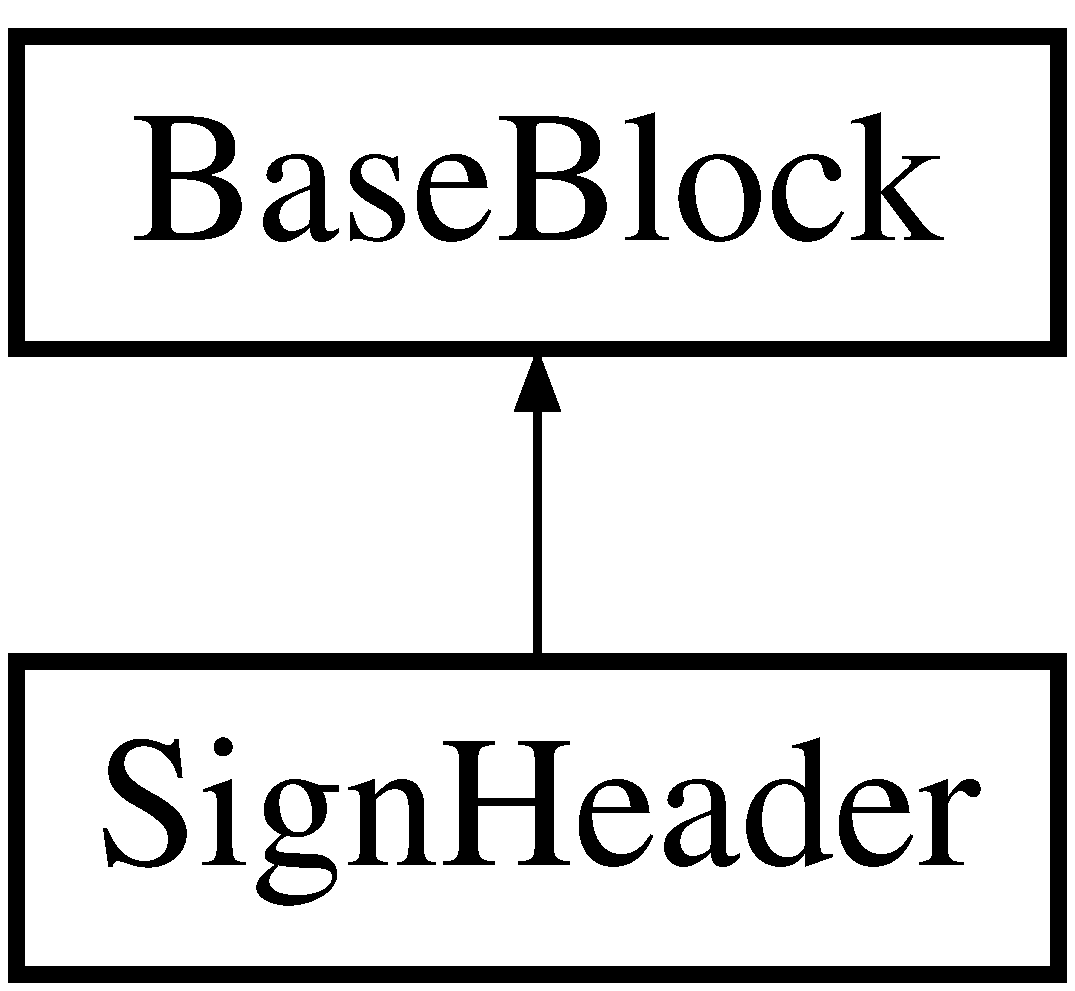
\includegraphics[height=2.000000cm]{struct_sign_header}
\end{center}
\end{figure}
\subsection*{Public Attributes}
\begin{DoxyCompactItemize}
\item 
\hypertarget{struct_sign_header_a591ec518ab2984a380de1e4436f3b61e}{uint {\bfseries Creation\-Time}}\label{struct_sign_header_a591ec518ab2984a380de1e4436f3b61e}

\item 
\hypertarget{struct_sign_header_ac60ed4404304fe729e211a64bdea81c3}{ushort {\bfseries Arc\-Name\-Size}}\label{struct_sign_header_ac60ed4404304fe729e211a64bdea81c3}

\item 
\hypertarget{struct_sign_header_a9aa61d3242fcf619f16e76a3de963b09}{ushort {\bfseries User\-Name\-Size}}\label{struct_sign_header_a9aa61d3242fcf619f16e76a3de963b09}

\end{DoxyCompactItemize}
\subsection*{Additional Inherited Members}


The documentation for this struct was generated from the following file\-:\begin{DoxyCompactItemize}
\item 
/\-Users/salazbr1/\-Documents/\-N\-P\-S/final\-\_\-unrarbulk\-\_\-extractor\-\_\-07-\/26-\/12/code/headers.\-hpp\end{DoxyCompactItemize}

\hypertarget{struct_s_t_a_t_e}{\section{S\-T\-A\-T\-E Struct Reference}
\label{struct_s_t_a_t_e}\index{S\-T\-A\-T\-E@{S\-T\-A\-T\-E}}
}
\subsection*{Public Attributes}
\begin{DoxyCompactItemize}
\item 
\hypertarget{struct_s_t_a_t_e_aac7291ecff7f2ff9a4c1de981b8dd031}{byte {\bfseries Symbol}}\label{struct_s_t_a_t_e_aac7291ecff7f2ff9a4c1de981b8dd031}

\item 
\hypertarget{struct_s_t_a_t_e_a737b0336d10eb53b73c112f02795285e}{byte {\bfseries Freq}}\label{struct_s_t_a_t_e_a737b0336d10eb53b73c112f02795285e}

\item 
\hypertarget{struct_s_t_a_t_e_a177ed959ff59e0b0fcc5f0177670da88}{\hyperlink{struct_p_p_m___c_o_n_t_e_x_t}{P\-P\-M\-\_\-\-C\-O\-N\-T\-E\-X\-T} $\ast$ {\bfseries Successor}}\label{struct_s_t_a_t_e_a177ed959ff59e0b0fcc5f0177670da88}

\end{DoxyCompactItemize}


The documentation for this struct was generated from the following file\-:\begin{DoxyCompactItemize}
\item 
/\-Users/salazbr1/\-Documents/\-N\-P\-S/final\-\_\-unrarbulk\-\_\-extractor\-\_\-07-\/26-\/12/code/model.\-hpp\end{DoxyCompactItemize}

\hypertarget{struct_stream_header}{\section{Stream\-Header Struct Reference}
\label{struct_stream_header}\index{Stream\-Header@{Stream\-Header}}
}
Inheritance diagram for Stream\-Header\-:\begin{figure}[H]
\begin{center}
\leavevmode
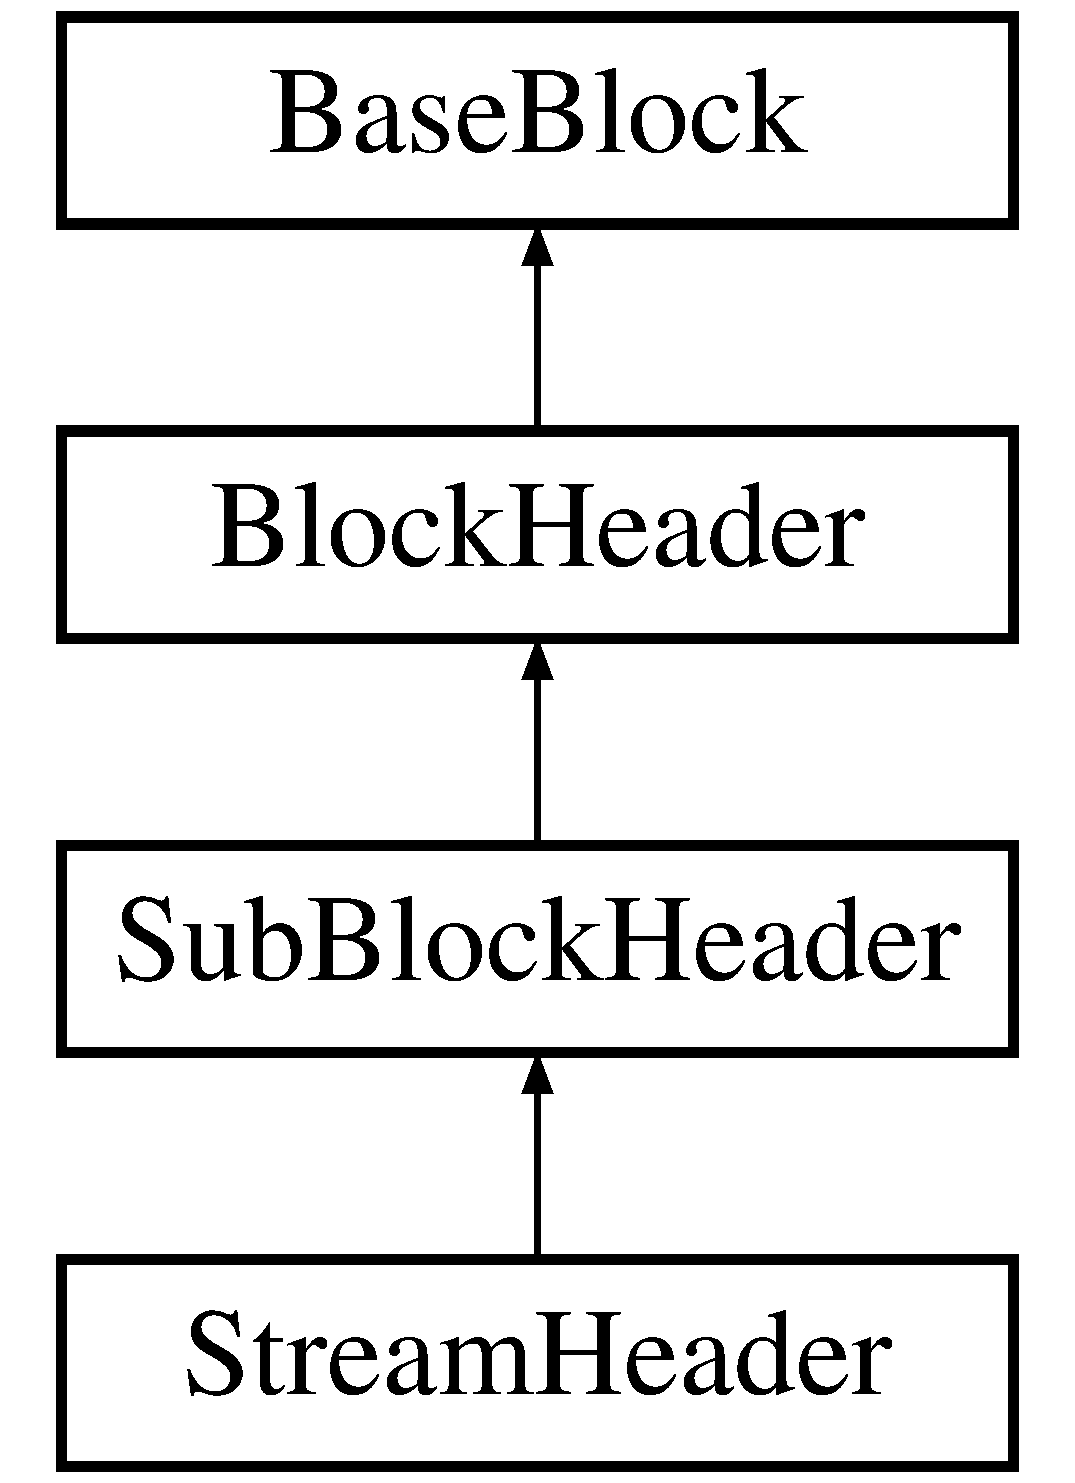
\includegraphics[height=4.000000cm]{struct_stream_header}
\end{center}
\end{figure}
\subsection*{Public Attributes}
\begin{DoxyCompactItemize}
\item 
\hypertarget{struct_stream_header_a73d4e2e55da2a1cd67ac689953fa8267}{uint {\bfseries Unp\-Size}}\label{struct_stream_header_a73d4e2e55da2a1cd67ac689953fa8267}

\item 
\hypertarget{struct_stream_header_aaab515ea2c0fa4a157b7cb5703777734}{byte {\bfseries Unp\-Ver}}\label{struct_stream_header_aaab515ea2c0fa4a157b7cb5703777734}

\item 
\hypertarget{struct_stream_header_aae812161c8878f4e619506b8584a282d}{byte {\bfseries Method}}\label{struct_stream_header_aae812161c8878f4e619506b8584a282d}

\item 
\hypertarget{struct_stream_header_a3e6f5f9cf255825f078ffc5ab2970bca}{uint {\bfseries Stream\-C\-R\-C}}\label{struct_stream_header_a3e6f5f9cf255825f078ffc5ab2970bca}

\item 
\hypertarget{struct_stream_header_a9e021407fd9a3cb90dabfcca17473ff5}{ushort {\bfseries Stream\-Name\-Size}}\label{struct_stream_header_a9e021407fd9a3cb90dabfcca17473ff5}

\item 
\hypertarget{struct_stream_header_ae02fb4782fb0e98ef04a086b7d3994bc}{byte {\bfseries Stream\-Name} \mbox{[}N\-M\mbox{]}}\label{struct_stream_header_ae02fb4782fb0e98ef04a086b7d3994bc}

\end{DoxyCompactItemize}


The documentation for this struct was generated from the following file\-:\begin{DoxyCompactItemize}
\item 
/\-Users/salazbr1/\-Documents/\-N\-P\-S/final\-\_\-unrarbulk\-\_\-extractor\-\_\-07-\/26-\/12/code/headers.\-hpp\end{DoxyCompactItemize}

\hypertarget{class_string_list}{\section{String\-List Class Reference}
\label{class_string_list}\index{String\-List@{String\-List}}
}
\subsection*{Public Member Functions}
\begin{DoxyCompactItemize}
\item 
\hypertarget{class_string_list_ae2a1e5a54ac6f920f05dc154b0bee611}{void {\bfseries Reset} ()}\label{class_string_list_ae2a1e5a54ac6f920f05dc154b0bee611}

\item 
\hypertarget{class_string_list_aaf00b2e6b7e8d8b6ac2df5ad90046a59}{void {\bfseries Add\-String} (const char $\ast$Str)}\label{class_string_list_aaf00b2e6b7e8d8b6ac2df5ad90046a59}

\item 
\hypertarget{class_string_list_a70962c7f2a69debd1b338110690628e2}{void {\bfseries Add\-String} (const wchar $\ast$Str)}\label{class_string_list_a70962c7f2a69debd1b338110690628e2}

\item 
\hypertarget{class_string_list_a15ede35fd74110f4cb6a0f023542c87a}{void {\bfseries Add\-String} (const char $\ast$Str, const wchar $\ast$Str\-W)}\label{class_string_list_a15ede35fd74110f4cb6a0f023542c87a}

\item 
\hypertarget{class_string_list_a9a24c36805a70615159663bbdc9de118}{bool {\bfseries Get\-String} (char $\ast$Str, size\-\_\-t Max\-Length)}\label{class_string_list_a9a24c36805a70615159663bbdc9de118}

\item 
\hypertarget{class_string_list_a21e569f644867c3943ab4b77c70e5e89}{bool {\bfseries Get\-String} (wchar $\ast$Str, size\-\_\-t Max\-Length)}\label{class_string_list_a21e569f644867c3943ab4b77c70e5e89}

\item 
\hypertarget{class_string_list_a1f71bf3075b90299810a04d3ba036236}{bool {\bfseries Get\-String} (char $\ast$Str, wchar $\ast$Str\-W, size\-\_\-t Max\-Length)}\label{class_string_list_a1f71bf3075b90299810a04d3ba036236}

\item 
\hypertarget{class_string_list_a10d8427780e2c0829958bb470f669190}{bool {\bfseries Get\-String} (char $\ast$Str, wchar $\ast$Str\-W, size\-\_\-t Max\-Length, int String\-Num)}\label{class_string_list_a10d8427780e2c0829958bb470f669190}

\item 
\hypertarget{class_string_list_a8ce858075112fbc5c2b7b814583a7dbe}{char $\ast$ {\bfseries Get\-String} ()}\label{class_string_list_a8ce858075112fbc5c2b7b814583a7dbe}

\item 
\hypertarget{class_string_list_af1352147021fc1455e68f962c589fcc8}{wchar $\ast$ {\bfseries Get\-String\-W} ()}\label{class_string_list_af1352147021fc1455e68f962c589fcc8}

\item 
\hypertarget{class_string_list_a396bcb354ab0dab47532a703bad62834}{bool {\bfseries Get\-String} (char $\ast$$\ast$Str, wchar $\ast$$\ast$Str\-W)}\label{class_string_list_a396bcb354ab0dab47532a703bad62834}

\item 
\hypertarget{class_string_list_a5141a3a9babf5fa7b488e0351c2c074f}{void {\bfseries Rewind} ()}\label{class_string_list_a5141a3a9babf5fa7b488e0351c2c074f}

\item 
\hypertarget{class_string_list_aa7af0e4098ea677cbdcadd061749fad4}{uint {\bfseries Items\-Count} ()}\label{class_string_list_aa7af0e4098ea677cbdcadd061749fad4}

\item 
\hypertarget{class_string_list_ad93731924716e97eac58e7f78616eb54}{size\-\_\-t {\bfseries Get\-Char\-Count} ()}\label{class_string_list_ad93731924716e97eac58e7f78616eb54}

\item 
\hypertarget{class_string_list_a3b87fa661a10de116b87f9c2023f154b}{bool {\bfseries Search} (char $\ast$Str, wchar $\ast$Str\-W, bool Case\-Sensitive)}\label{class_string_list_a3b87fa661a10de116b87f9c2023f154b}

\item 
\hypertarget{class_string_list_afb00ef6bf5dc0f62911f6c2ca92bbeb5}{void {\bfseries Save\-Position} ()}\label{class_string_list_afb00ef6bf5dc0f62911f6c2ca92bbeb5}

\item 
\hypertarget{class_string_list_a210e5a7bf506e3a41d443664f7fc35a5}{void {\bfseries Restore\-Position} ()}\label{class_string_list_a210e5a7bf506e3a41d443664f7fc35a5}

\end{DoxyCompactItemize}


The documentation for this class was generated from the following files\-:\begin{DoxyCompactItemize}
\item 
/\-Users/salazbr1/\-Documents/\-N\-P\-S/final\-\_\-unrarbulk\-\_\-extractor\-\_\-07-\/26-\/12/code/strlist.\-hpp\item 
/\-Users/salazbr1/\-Documents/\-N\-P\-S/final\-\_\-unrarbulk\-\_\-extractor\-\_\-07-\/26-\/12/code/strlist.\-cpp\end{DoxyCompactItemize}

\hypertarget{class_sub_allocator}{\section{Sub\-Allocator Class Reference}
\label{class_sub_allocator}\index{Sub\-Allocator@{Sub\-Allocator}}
}
\subsection*{Public Member Functions}
\begin{DoxyCompactItemize}
\item 
\hypertarget{class_sub_allocator_a212c556a0af59fed290008a88007ad2c}{void {\bfseries Clean} ()}\label{class_sub_allocator_a212c556a0af59fed290008a88007ad2c}

\item 
\hypertarget{class_sub_allocator_ab8065281115597696cf1b7c259cafc43}{bool {\bfseries Start\-Sub\-Allocator} (int S\-A\-Size)}\label{class_sub_allocator_ab8065281115597696cf1b7c259cafc43}

\item 
\hypertarget{class_sub_allocator_aac677cfd44f4efc22f792d197f69f7e6}{void {\bfseries Stop\-Sub\-Allocator} ()}\label{class_sub_allocator_aac677cfd44f4efc22f792d197f69f7e6}

\item 
\hypertarget{class_sub_allocator_a59f279eac051c2f489a06ba7aedc2d94}{void {\bfseries Init\-Sub\-Allocator} ()}\label{class_sub_allocator_a59f279eac051c2f489a06ba7aedc2d94}

\item 
\hypertarget{class_sub_allocator_ad4bc0686b9b2b01913e8c574956aa403}{void $\ast$ {\bfseries Alloc\-Context} ()}\label{class_sub_allocator_ad4bc0686b9b2b01913e8c574956aa403}

\item 
\hypertarget{class_sub_allocator_ae601b3aa72108ebf20f4de8c1b75a6c8}{void $\ast$ {\bfseries Alloc\-Units} (int N\-U)}\label{class_sub_allocator_ae601b3aa72108ebf20f4de8c1b75a6c8}

\item 
\hypertarget{class_sub_allocator_a43a8793154fdffe04e05ca8b15700dd5}{void $\ast$ {\bfseries Expand\-Units} (void $\ast$ptr, int Old\-N\-U)}\label{class_sub_allocator_a43a8793154fdffe04e05ca8b15700dd5}

\item 
\hypertarget{class_sub_allocator_aa1bd219580ce6e1bc2b42b1436a22238}{void $\ast$ {\bfseries Shrink\-Units} (void $\ast$ptr, int Old\-N\-U, int New\-N\-U)}\label{class_sub_allocator_aa1bd219580ce6e1bc2b42b1436a22238}

\item 
\hypertarget{class_sub_allocator_a4ad0e2df3064e52bbfae963c41ae7c6c}{void {\bfseries Free\-Units} (void $\ast$ptr, int Old\-N\-U)}\label{class_sub_allocator_a4ad0e2df3064e52bbfae963c41ae7c6c}

\item 
\hypertarget{class_sub_allocator_a98aba9288cdfc643486c65794d97a865}{long {\bfseries Get\-Allocated\-Memory} ()}\label{class_sub_allocator_a98aba9288cdfc643486c65794d97a865}

\end{DoxyCompactItemize}
\subsection*{Public Attributes}
\begin{DoxyCompactItemize}
\item 
\hypertarget{class_sub_allocator_a38eca006c5fc86d70be3278a28e1fb73}{byte $\ast$ {\bfseries p\-Text}}\label{class_sub_allocator_a38eca006c5fc86d70be3278a28e1fb73}

\item 
\hypertarget{class_sub_allocator_accd9fa3946e8b71af00e6484afb711a1}{byte $\ast$ {\bfseries Units\-Start}}\label{class_sub_allocator_accd9fa3946e8b71af00e6484afb711a1}

\item 
\hypertarget{class_sub_allocator_a5cbcfb8037403a6d06cf50236fa278c7}{byte $\ast$ {\bfseries Heap\-End}}\label{class_sub_allocator_a5cbcfb8037403a6d06cf50236fa278c7}

\item 
\hypertarget{class_sub_allocator_a90ed7682a5ab2da5f8b051e98f0c9e59}{byte $\ast$ {\bfseries Fake\-Units\-Start}}\label{class_sub_allocator_a90ed7682a5ab2da5f8b051e98f0c9e59}

\end{DoxyCompactItemize}


The documentation for this class was generated from the following files\-:\begin{DoxyCompactItemize}
\item 
/\-Users/salazbr1/\-Documents/\-N\-P\-S/final\-\_\-unrarbulk\-\_\-extractor\-\_\-07-\/26-\/12/code/suballoc.\-hpp\item 
/\-Users/salazbr1/\-Documents/\-N\-P\-S/final\-\_\-unrarbulk\-\_\-extractor\-\_\-07-\/26-\/12/code/suballoc.\-cpp\end{DoxyCompactItemize}

\hypertarget{struct_sub_block_header}{\section{Sub\-Block\-Header Struct Reference}
\label{struct_sub_block_header}\index{Sub\-Block\-Header@{Sub\-Block\-Header}}
}
Inheritance diagram for Sub\-Block\-Header\-:\begin{figure}[H]
\begin{center}
\leavevmode
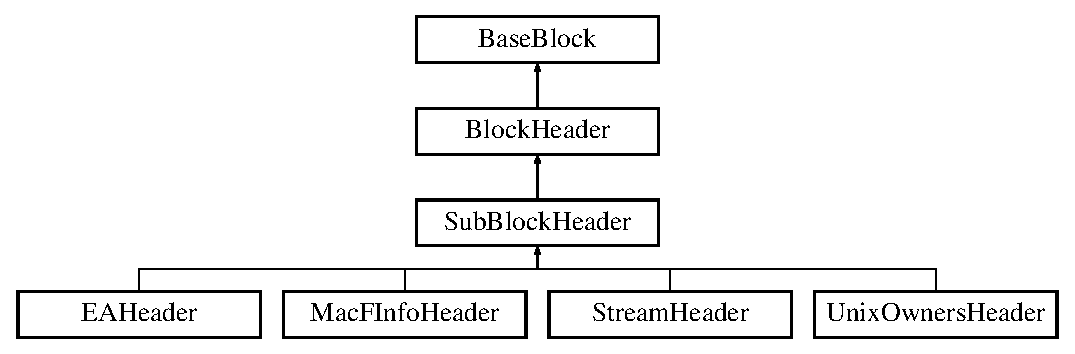
\includegraphics[height=4.000000cm]{struct_sub_block_header}
\end{center}
\end{figure}
\subsection*{Public Attributes}
\begin{DoxyCompactItemize}
\item 
\hypertarget{struct_sub_block_header_a74376e79e3058ed772ec9d23144749ae}{ushort {\bfseries Sub\-Type}}\label{struct_sub_block_header_a74376e79e3058ed772ec9d23144749ae}

\item 
\hypertarget{struct_sub_block_header_a26a4bdc742f6c521058089ac5be2da28}{byte {\bfseries Level}}\label{struct_sub_block_header_a26a4bdc742f6c521058089ac5be2da28}

\end{DoxyCompactItemize}


The documentation for this struct was generated from the following file\-:\begin{DoxyCompactItemize}
\item 
/\-Users/salazbr1/\-Documents/\-N\-P\-S/final\-\_\-unrarbulk\-\_\-extractor\-\_\-07-\/26-\/12/code/headers.\-hpp\end{DoxyCompactItemize}

\hypertarget{struct_range_coder_1_1_s_u_b_r_a_n_g_e}{\section{Range\-Coder\-:\-:S\-U\-B\-R\-A\-N\-G\-E Struct Reference}
\label{struct_range_coder_1_1_s_u_b_r_a_n_g_e}\index{Range\-Coder\-::\-S\-U\-B\-R\-A\-N\-G\-E@{Range\-Coder\-::\-S\-U\-B\-R\-A\-N\-G\-E}}
}
\subsection*{Public Attributes}
\begin{DoxyCompactItemize}
\item 
\hypertarget{struct_range_coder_1_1_s_u_b_r_a_n_g_e_a11578b7f095d8565fd7efe6be2de12bb}{uint {\bfseries Low\-Count}}\label{struct_range_coder_1_1_s_u_b_r_a_n_g_e_a11578b7f095d8565fd7efe6be2de12bb}

\item 
\hypertarget{struct_range_coder_1_1_s_u_b_r_a_n_g_e_a554e99044a999428f02382a29ce11dee}{uint {\bfseries High\-Count}}\label{struct_range_coder_1_1_s_u_b_r_a_n_g_e_a554e99044a999428f02382a29ce11dee}

\item 
\hypertarget{struct_range_coder_1_1_s_u_b_r_a_n_g_e_abee4afcbcde5137dc02a6b45248e6207}{uint {\bfseries scale}}\label{struct_range_coder_1_1_s_u_b_r_a_n_g_e_abee4afcbcde5137dc02a6b45248e6207}

\end{DoxyCompactItemize}


The documentation for this struct was generated from the following file\-:\begin{DoxyCompactItemize}
\item 
/\-Users/salazbr1/\-Documents/\-N\-P\-S/final\-\_\-unrarbulk\-\_\-extractor\-\_\-07-\/26-\/12/code/coder.\-hpp\end{DoxyCompactItemize}

\hypertarget{struct_unix_owners_header}{\section{Unix\-Owners\-Header Struct Reference}
\label{struct_unix_owners_header}\index{Unix\-Owners\-Header@{Unix\-Owners\-Header}}
}
Inheritance diagram for Unix\-Owners\-Header\-:\begin{figure}[H]
\begin{center}
\leavevmode
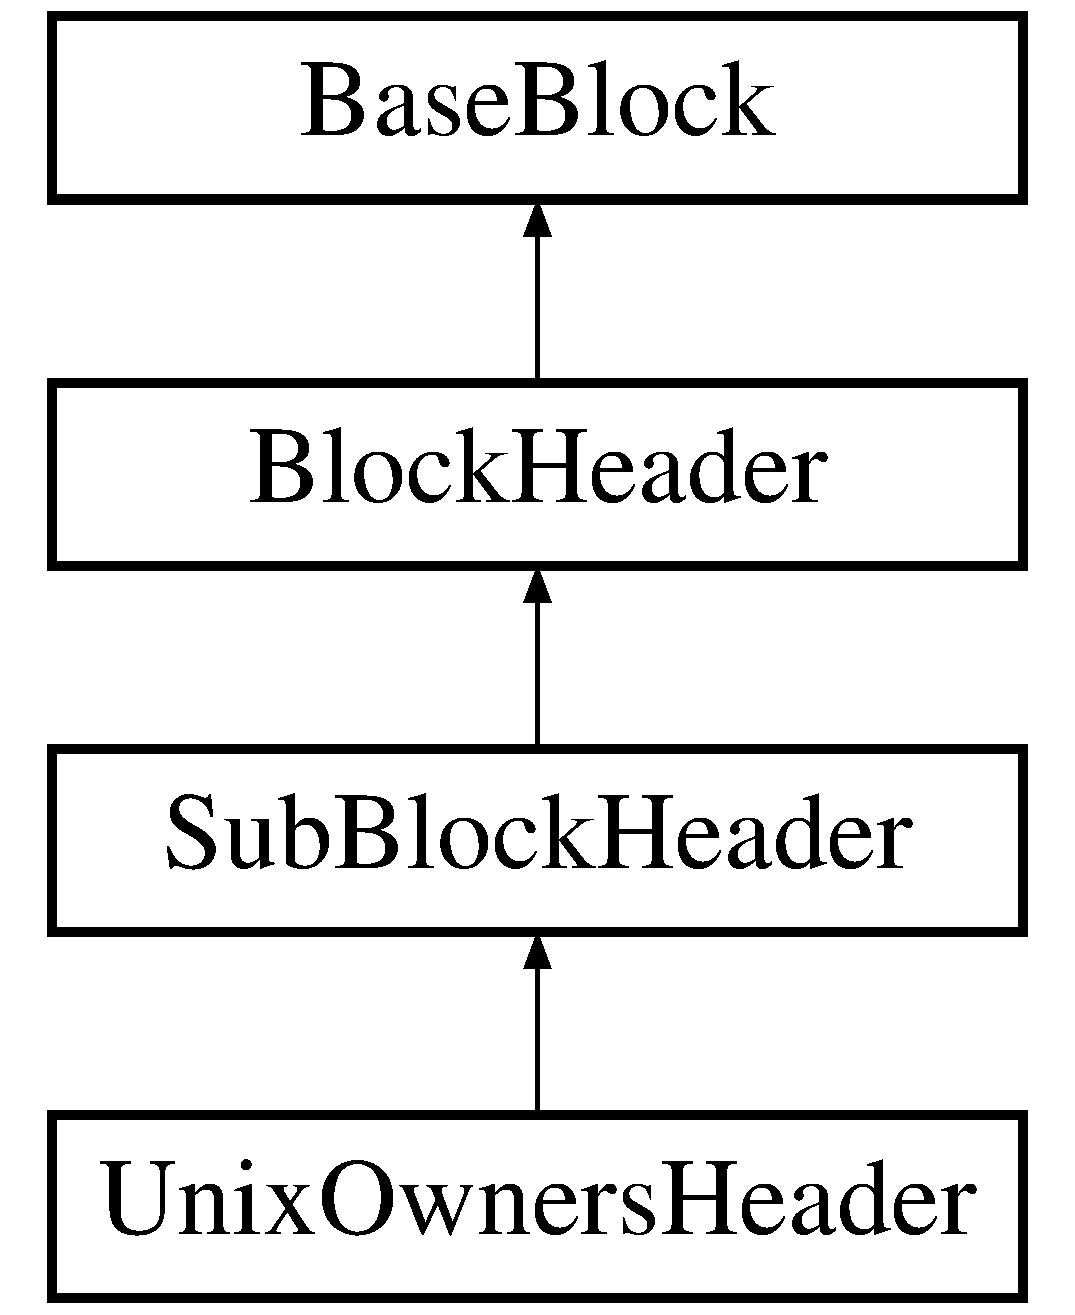
\includegraphics[height=4.000000cm]{struct_unix_owners_header}
\end{center}
\end{figure}
\subsection*{Public Attributes}
\begin{DoxyCompactItemize}
\item 
\hypertarget{struct_unix_owners_header_a7a873745d81d6fca11eb96a6089c22fa}{ushort {\bfseries Owner\-Name\-Size}}\label{struct_unix_owners_header_a7a873745d81d6fca11eb96a6089c22fa}

\item 
\hypertarget{struct_unix_owners_header_a2181313771b87e5f594a5b5d97b6ee53}{ushort {\bfseries Group\-Name\-Size}}\label{struct_unix_owners_header_a2181313771b87e5f594a5b5d97b6ee53}

\item 
\hypertarget{struct_unix_owners_header_a069ae6faf222464bcff8b10417e2aa39}{char {\bfseries Owner\-Name} \mbox{[}N\-M\mbox{]}}\label{struct_unix_owners_header_a069ae6faf222464bcff8b10417e2aa39}

\item 
\hypertarget{struct_unix_owners_header_a7561551724fdf362c444b24aab4a327d}{char {\bfseries Group\-Name} \mbox{[}N\-M\mbox{]}}\label{struct_unix_owners_header_a7561551724fdf362c444b24aab4a327d}

\end{DoxyCompactItemize}


The documentation for this struct was generated from the following file\-:\begin{DoxyCompactItemize}
\item 
/\-Users/salazbr1/\-Documents/\-N\-P\-S/final\-\_\-unrarbulk\-\_\-extractor\-\_\-07-\/26-\/12/code/headers.\-hpp\end{DoxyCompactItemize}

\hypertarget{class_unpack}{\section{Unpack Class Reference}
\label{class_unpack}\index{Unpack@{Unpack}}
}
Inheritance diagram for Unpack\-:\begin{figure}[H]
\begin{center}
\leavevmode
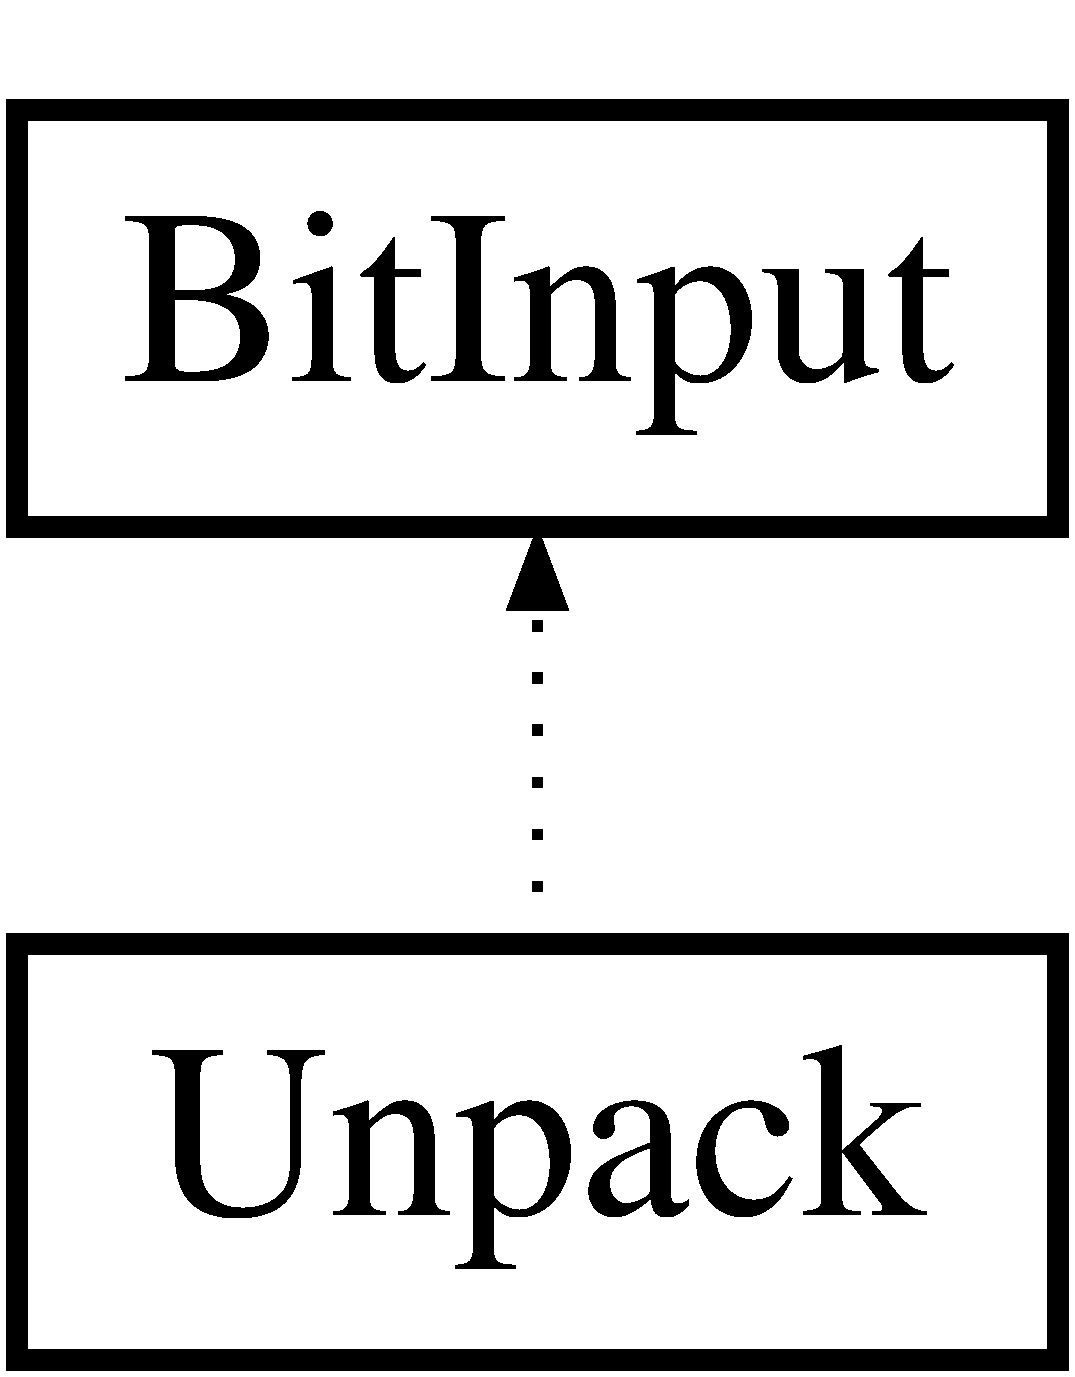
\includegraphics[height=2.000000cm]{class_unpack}
\end{center}
\end{figure}
\subsection*{Public Member Functions}
\begin{DoxyCompactItemize}
\item 
\hypertarget{class_unpack_af5593e68f5e3e295a625555827e43fc1}{{\bfseries Unpack} (\hyperlink{class_compr_data_i_o}{Compr\-Data\-I\-O} $\ast$Data\-I\-O)}\label{class_unpack_af5593e68f5e3e295a625555827e43fc1}

\item 
\hypertarget{class_unpack_a05f04f77abe389b1d755771ca3df3b56}{void {\bfseries Init} (byte $\ast$Window=N\-U\-L\-L)}\label{class_unpack_a05f04f77abe389b1d755771ca3df3b56}

\item 
\hypertarget{class_unpack_ab0891c4f27fc029dc185b68d164f91ea}{void {\bfseries Do\-Unpack} (int Method, bool Solid)}\label{class_unpack_ab0891c4f27fc029dc185b68d164f91ea}

\item 
\hypertarget{class_unpack_a9ffdd702fc7a20cbd09bae52d5817bfe}{bool {\bfseries Is\-File\-Extracted} ()}\label{class_unpack_a9ffdd702fc7a20cbd09bae52d5817bfe}

\item 
\hypertarget{class_unpack_ab7415d69f73a5c29638dd14a091f2414}{void {\bfseries Set\-Dest\-Size} (int64 Dest\-Size)}\label{class_unpack_ab7415d69f73a5c29638dd14a091f2414}

\item 
\hypertarget{class_unpack_a80b0c836f1f795dca8e7f0a9ea9405a5}{void {\bfseries Set\-Suspended} (bool Suspended)}\label{class_unpack_a80b0c836f1f795dca8e7f0a9ea9405a5}

\item 
\hypertarget{class_unpack_a9af22d08aec9134c7b878ea4ddc21dc4}{unsigned int {\bfseries Get\-Char} ()}\label{class_unpack_a9af22d08aec9134c7b878ea4ddc21dc4}

\end{DoxyCompactItemize}
\subsection*{Friends}
\begin{DoxyCompactItemize}
\item 
\hypertarget{class_unpack_ac043485674645a0ae476481e1fdec631}{class {\bfseries Pack}}\label{class_unpack_ac043485674645a0ae476481e1fdec631}

\end{DoxyCompactItemize}
\subsection*{Additional Inherited Members}


The documentation for this class was generated from the following files\-:\begin{DoxyCompactItemize}
\item 
/\-Users/salazbr1/\-Documents/\-N\-P\-S/final\-\_\-unrarbulk\-\_\-extractor\-\_\-07-\/26-\/12/code/unpack.\-hpp\item 
/\-Users/salazbr1/\-Documents/\-N\-P\-S/final\-\_\-unrarbulk\-\_\-extractor\-\_\-07-\/26-\/12/code/unpack.\-cpp\item 
/\-Users/salazbr1/\-Documents/\-N\-P\-S/final\-\_\-unrarbulk\-\_\-extractor\-\_\-07-\/26-\/12/code/unpack15.\-cpp\item 
/\-Users/salazbr1/\-Documents/\-N\-P\-S/final\-\_\-unrarbulk\-\_\-extractor\-\_\-07-\/26-\/12/code/unpack20.\-cpp\end{DoxyCompactItemize}

\hypertarget{struct_unpack_filter}{\section{Unpack\-Filter Struct Reference}
\label{struct_unpack_filter}\index{Unpack\-Filter@{Unpack\-Filter}}
}
\subsection*{Public Attributes}
\begin{DoxyCompactItemize}
\item 
\hypertarget{struct_unpack_filter_a368b53188fbd6301c5f9f8c6b7c102eb}{unsigned int {\bfseries Block\-Start}}\label{struct_unpack_filter_a368b53188fbd6301c5f9f8c6b7c102eb}

\item 
\hypertarget{struct_unpack_filter_a06ab8d48d3d41aa1bf4f87c4a4ad9968}{unsigned int {\bfseries Block\-Length}}\label{struct_unpack_filter_a06ab8d48d3d41aa1bf4f87c4a4ad9968}

\item 
\hypertarget{struct_unpack_filter_a839710e5c94b13f658b3489e10cf0362}{unsigned int {\bfseries Exec\-Count}}\label{struct_unpack_filter_a839710e5c94b13f658b3489e10cf0362}

\item 
\hypertarget{struct_unpack_filter_a10816e5c9e32126fac0b39707d7b8acd}{bool {\bfseries Next\-Window}}\label{struct_unpack_filter_a10816e5c9e32126fac0b39707d7b8acd}

\item 
\hypertarget{struct_unpack_filter_a070d0aa66673287f04c23e8eaaaeb0e2}{unsigned int {\bfseries Parent\-Filter}}\label{struct_unpack_filter_a070d0aa66673287f04c23e8eaaaeb0e2}

\item 
\hypertarget{struct_unpack_filter_ad74355f58bb17a9d052e668cad46489a}{\hyperlink{struct_v_m___prepared_program}{V\-M\-\_\-\-Prepared\-Program} {\bfseries Prg}}\label{struct_unpack_filter_ad74355f58bb17a9d052e668cad46489a}

\end{DoxyCompactItemize}


The documentation for this struct was generated from the following file\-:\begin{DoxyCompactItemize}
\item 
/\-Users/salazbr1/\-Documents/\-N\-P\-S/final\-\_\-unrarbulk\-\_\-extractor\-\_\-07-\/26-\/12/code/unpack.\-hpp\end{DoxyCompactItemize}

\hypertarget{struct_v_m___prepared_command}{\section{V\-M\-\_\-\-Prepared\-Command Struct Reference}
\label{struct_v_m___prepared_command}\index{V\-M\-\_\-\-Prepared\-Command@{V\-M\-\_\-\-Prepared\-Command}}
}
\subsection*{Public Attributes}
\begin{DoxyCompactItemize}
\item 
\hypertarget{struct_v_m___prepared_command_aa435fdb81435ccba7dd8dc9251a5464b}{V\-M\-\_\-\-Commands {\bfseries Op\-Code}}\label{struct_v_m___prepared_command_aa435fdb81435ccba7dd8dc9251a5464b}

\item 
\hypertarget{struct_v_m___prepared_command_a24b622f3a976111f41d471096669422c}{bool {\bfseries Byte\-Mode}}\label{struct_v_m___prepared_command_a24b622f3a976111f41d471096669422c}

\item 
\hypertarget{struct_v_m___prepared_command_a1a7c0eeee1b506f0bf6e1b21d3a7e8f9}{\hyperlink{struct_v_m___prepared_operand}{V\-M\-\_\-\-Prepared\-Operand} {\bfseries Op1}}\label{struct_v_m___prepared_command_a1a7c0eeee1b506f0bf6e1b21d3a7e8f9}

\item 
\hypertarget{struct_v_m___prepared_command_aa32d907ab68f7af12164876dc6ab628c}{\hyperlink{struct_v_m___prepared_operand}{V\-M\-\_\-\-Prepared\-Operand} {\bfseries Op2}}\label{struct_v_m___prepared_command_aa32d907ab68f7af12164876dc6ab628c}

\end{DoxyCompactItemize}


The documentation for this struct was generated from the following file\-:\begin{DoxyCompactItemize}
\item 
/\-Users/salazbr1/\-Documents/\-N\-P\-S/final\-\_\-unrarbulk\-\_\-extractor\-\_\-07-\/26-\/12/code/rarvm.\-hpp\end{DoxyCompactItemize}

\hypertarget{struct_v_m___prepared_operand}{\section{V\-M\-\_\-\-Prepared\-Operand Struct Reference}
\label{struct_v_m___prepared_operand}\index{V\-M\-\_\-\-Prepared\-Operand@{V\-M\-\_\-\-Prepared\-Operand}}
}
\subsection*{Public Attributes}
\begin{DoxyCompactItemize}
\item 
\hypertarget{struct_v_m___prepared_operand_a80352e8ed7473a3d8561f8887ed40474}{V\-M\-\_\-\-Op\-Type {\bfseries Type}}\label{struct_v_m___prepared_operand_a80352e8ed7473a3d8561f8887ed40474}

\item 
\hypertarget{struct_v_m___prepared_operand_a7549a42c9592d8013cc07b74b82ddf61}{uint {\bfseries Data}}\label{struct_v_m___prepared_operand_a7549a42c9592d8013cc07b74b82ddf61}

\item 
\hypertarget{struct_v_m___prepared_operand_a019341ad00e2ea1b4a3a9510a3a59542}{uint {\bfseries Base}}\label{struct_v_m___prepared_operand_a019341ad00e2ea1b4a3a9510a3a59542}

\item 
\hypertarget{struct_v_m___prepared_operand_a63decb06e755883cf805c744993659d6}{uint $\ast$ {\bfseries Addr}}\label{struct_v_m___prepared_operand_a63decb06e755883cf805c744993659d6}

\end{DoxyCompactItemize}


The documentation for this struct was generated from the following file\-:\begin{DoxyCompactItemize}
\item 
/\-Users/salazbr1/\-Documents/\-N\-P\-S/final\-\_\-unrarbulk\-\_\-extractor\-\_\-07-\/26-\/12/code/rarvm.\-hpp\end{DoxyCompactItemize}

\hypertarget{struct_v_m___prepared_program}{\section{V\-M\-\_\-\-Prepared\-Program Struct Reference}
\label{struct_v_m___prepared_program}\index{V\-M\-\_\-\-Prepared\-Program@{V\-M\-\_\-\-Prepared\-Program}}
}
\subsection*{Public Attributes}
\begin{DoxyCompactItemize}
\item 
\hypertarget{struct_v_m___prepared_program_a54c5136bd73958a64606e3568c543a92}{\hyperlink{class_array}{Array}$<$ \hyperlink{struct_v_m___prepared_command}{V\-M\-\_\-\-Prepared\-Command} $>$ {\bfseries Cmd}}\label{struct_v_m___prepared_program_a54c5136bd73958a64606e3568c543a92}

\item 
\hypertarget{struct_v_m___prepared_program_a88c47f348c4f1b9a5469d3361827b376}{\hyperlink{struct_v_m___prepared_command}{V\-M\-\_\-\-Prepared\-Command} $\ast$ {\bfseries Alt\-Cmd}}\label{struct_v_m___prepared_program_a88c47f348c4f1b9a5469d3361827b376}

\item 
\hypertarget{struct_v_m___prepared_program_a43b01e89ea2d2ac6d3c30490fd27b008}{int {\bfseries Cmd\-Count}}\label{struct_v_m___prepared_program_a43b01e89ea2d2ac6d3c30490fd27b008}

\item 
\hypertarget{struct_v_m___prepared_program_a40936f34ce73f7d05701a2810778c226}{\hyperlink{class_array}{Array}$<$ byte $>$ {\bfseries Global\-Data}}\label{struct_v_m___prepared_program_a40936f34ce73f7d05701a2810778c226}

\item 
\hypertarget{struct_v_m___prepared_program_a3e7e7e9d4a094f129b1aabc31191a8b4}{\hyperlink{class_array}{Array}$<$ byte $>$ {\bfseries Static\-Data}}\label{struct_v_m___prepared_program_a3e7e7e9d4a094f129b1aabc31191a8b4}

\item 
\hypertarget{struct_v_m___prepared_program_a32e939a51a067a83084538b0c14bb515}{uint {\bfseries Init\-R} \mbox{[}7\mbox{]}}\label{struct_v_m___prepared_program_a32e939a51a067a83084538b0c14bb515}

\item 
\hypertarget{struct_v_m___prepared_program_aeae9193fc13999b6fe5f5db3e99c1d93}{byte $\ast$ {\bfseries Filtered\-Data}}\label{struct_v_m___prepared_program_aeae9193fc13999b6fe5f5db3e99c1d93}

\item 
\hypertarget{struct_v_m___prepared_program_ae07dc4e3c379d36c5dd9cdca6f47cb16}{uint {\bfseries Filtered\-Data\-Size}}\label{struct_v_m___prepared_program_ae07dc4e3c379d36c5dd9cdca6f47cb16}

\end{DoxyCompactItemize}


The documentation for this struct was generated from the following file\-:\begin{DoxyCompactItemize}
\item 
/\-Users/salazbr1/\-Documents/\-N\-P\-S/final\-\_\-unrarbulk\-\_\-extractor\-\_\-07-\/26-\/12/code/rarvm.\-hpp\end{DoxyCompactItemize}

\printindex
\end{document}
